\documentclass[UKenglish]{uiomasterthesis}
\usepackage{{booktabs}}
\usepackage{algpseudocode}
\usepackage{algorithm}
\usepackage{graphicx} 
\usepackage[UKenglish]{uiomasterfp}
\usepackage[nottoc]{tocbibind}
\usepackage[hidelinks]{hyperref}
\usepackage{amsmath}
\usepackage{amsfonts}
\usepackage[printonlyused]{acronym}
\usepackage{tikz}
\usepackage{pgfplots} 
\usepackage[backend=biber, style=numeric-comp, sorting=none]{biblatex}
\addbibresource{ref.bib}
\usetikzlibrary{arrows, arrows.meta, positioning, calc}
\usepackage{listofitems}


\title{Explainable Reinforcement Learning}
\subtitle{Discovering intent based explanations for heterogeneous cooperative multi agent reinforcement learning agents}
\author{Ada Hatland}
\date{August 2024}


\pagenumbering{roman}

\begin{document}

\uiomasterfp[master, program={Informatics: Robotics and Intelligent Systems},
  color=orange, dept={Department of Informatics}, fac={The Faculty of Mathematics and Natural Sciences},
  supervisors={Dr. Dennis Gro\ss \and Prof. Kyrre Glette\and Dr. Helge Spieker}, image = {images/cat.png}]

\renewcommand*\acffont{\textit}

\section*{Declaration of AI use}
In this thesis generative models have been used for topic suggestion, a small part of figure creation, equations and parts of the code used for creating plots, as well as debugging and documentation. All code suggested has been verified by a human. Generative models have \textbf{not} been used for text generation. I, the author, take full responsibility for the contents of this thesis.


\section*{Acknowledgments}
I would like to thank my external supervisor Dennis Gro\ss, as well as my internal supervisor Kyrre Glette for their guidance and support in writing this thesis. They have been of significant help when discussing how to proceed and what remains on the to-do list. I would also like to thank my cat Nokia for emotional support throughout the writing of this thesis.

\section*{List of Acronyms}
\begin{acronym}[ICANN]
    \acro  {rl}   [RL]   {Reinforcement Learning}
    \acro  {xrl} [XRL] {Explainable Reinforcement Learning}
    \acro  {ai}   [AI]   {Artificial Intelligence}
    \acro  {xai}  [XAI]  {Explainable Artificial Intelligence}
    \acro  {marl}  [MARL]  {Multi Agent Reinforcement Learning}
    \acro  {mdp}  [MDP]  {Markov Decision Process}
    \acro  {dqn}  [DQN]  {Deep Q-Network}
    \acro  {ppo}  [PPO]  {Proximal Policy Optimization}
    \acro  {drl}  [DRL]  {Deep Reinforcement Learning}
    \acro  {rnn}  [RNN]  {Recurrent Neural Network}
    \acro  {lstm}  [LSTM]  {Long Short Term Memory}
    \acro  {mbrl}  [MBRL]  {Model-Based Reinforcement Learning}
    \acro  {llm}  [LLM]  {Large Language Model}
    \acro  {ea}  [EA]  {Evolutionary Algorithm}
    \acro  {nsga}  [NSGA-II]  {Non-Dominated Sorting Genetic Algorithm II}
    \acro  {nn}  [NN]  {Neural Network}
    \acro  {aec}  [AEC]  {Agent Environment Cycle}
    \acro  {cnn}  [CNN]  {Convolutional Neural Network}
    \acro  {drc}  [DRC]  {Deep Repeated ConvLSTM}
    \acro  {pomdp}  [POMDP]  {Partially Observable Markov Decision Process}
\end{acronym}


\abstract
This is the abstract

\lefthyphenmin=1000
\tableofcontents
\listoftables
\listoffigures
\chapter{Introduction}

\pagenumbering{arabic}

Sequential decision-making problems are problems where one decision leads to a new state that requires a new decision to be made. An example of this is autonomously driving from point A to point B through city streets. For these types of problems \ac{rl} systems are used. \ac{rl}, both multi- and single-agent models have seen a significant rise in successful use and applicability in recent years, with models such as AlphaGo\cite{article} and smacv2\cite{ellis2023smacv2}. These models learn by agents performing actions in a given state decided by a policy that lead to a new state, and learning by receiving rewards depending on if the new state is preferable to the previous, the aim is to learn a near optimal policy for achieving a fixed goal\cite{Sutton1998}. The agent uses an observation of the state to choose an action. The environment describes how an action affects the state. See Figure \ref{fig:rl_basics}. In a \ac{marl} system, we would have multiple agents.

\section{Motivation}
\label{sec:motivation}
A significant problem with many deep machine learning models, including \ac{marl} policies, is known as the black box problem\cite{zednik2019solving}. This problem describes how the processing of information is hidden from a human user due to the opacity of the model, and we just have to trust that the model uses relevant data to come to the conclusion it does, which it often doesn't do. For many tasks and models where the impact of the output isn't highly significant this isn't a big issue, but for tasks like autonomous driving we simply cannot use these models without trust for the models processing of data and that the solution given wont hurt anyone. We can considering autonomous driving as a \ac{marl} system if we consider each vehicle as an agent. To solve this we would like to have models that along with an output can provide us with some kind of reasoning for what information is used and how.

All this essentially means, until the black box problem is solved, autopilot will always require a driver behind the wheel\cite{tian2018deeptest}. Despite having high accuracy, precision and recall, a reinforcement learning model might choose a less than preferable action in edge cases or states not well covered by training and test sets, for example driving on snowy roads when all images in the training data is from warmer climates, or combinations that aren't well covered, like a foggy, snowy road with a sharp right turn.
With a way to ask the agent for intent, we could find that it has learned to always expect there to not be a car around the corner, which is not always obvious from looking at the dataset, but if it in a decision relies on the road to be empty to choose a safe route, this is obviously a huge issue. This paper aims to explain how an agent in a \ac{marl} setting decides on an action due to what it expects from other agents in the future. The field working on combating this issue is known is Explainable reinforcement learning.

\section{Problem statement}
\label{sec:problem}
The focus of this paper will be to rework and apply methods for general \ac{xai} to Reinforcement Learning, and expand on \ac{xrl} methods already developed. In particular we will focus on an agent and how the expected future states of other agents will affect it in its decision making process. The environment we will focus on is a \ac{marl} environment known as Knights Archers Zombies \cite{KAZ} made for Python. We use this because it is a cooperative environment where each agent has to consider other agents, both of the same type as itself, and other types. If we used an environment where all the agents are identical, our findings will be less useful for other environments where the agents aren't identical. In many real life scenarios agents will not be identical. If we once again consider autonomous vehicles, most vehicles are different in some way. A very obvious example of this is considering cars and motorcycles. Where because of their size difference, their paths chosen will often be different.

In psychology it is well known that most human based decisions are made with intent\cite{inbook}, and by focusing on the expectation of what future states will look like we can consider this the intent of the agent. If we are accurately able to extract the intent of an \ac{rl} policy we are better able to explain the choice made and we are more comfortable with trusting that the choice made is a good decision. Concretely we hypothesise that by analyzing expected future states and events we could find the intent of the agent, which we could use to ensure the agent acts in a safe or desirable manner. The main question we aim to answer is what information, found in weights or design of the policy, or information extracted by knowing the weights and design, is the most important for separate prediction models to be able to predict future states and actions, in cases where we do not have access to a decent world model, or such a model does not exist.


\section{Scope and limitations}
We aim to construct a framework to describe the intent of the agents in the KAZ environment, and we aim to make it applicable to other environments as well. However, due to time limitations we restrict the framework to only accept PettingZoo example environments or environments created with the PettingZoo environment creation tool. \ac{marl} environments can be divided into two major categories, \ac{aec} and parallel. \ac{aec} environments are environments where the state transition happens after each agent chooses an action, and parallel environments are environments where all the agents choose an action each before the transition happens. See figure \ref{fig:aec}.

Due to limited time and resources the size of policy or value networks, as well as any other \acp{nn} or otherwise computationally expensive algorithm used, will have to be significantly limited, this will impact results in a meaningful way, and therefore we will keep all \acp{nn} comparable sizes, and focus on doing experiments on how other factors than network size impact the results.

We do not have access to any real world datasets, so its hard to ensure the methods we have developed will be directly applicable, however the results we get will still be relevant for later research in the area.
\begin{figure}
\begin{center}

\begin{tikzpicture}[>=Latex, node distance=2.5cm, auto, font=\small]

    % Agent 1 Node
    \node[draw, thick, circle, fill=blue!20, minimum size=2.5cm, align=center] (agent1)
    at (-3,3) {Agent 1 \\ \(\pi_{\theta_1}\)};

    % Transition 1 Node
    \node[draw, thick, circle, fill=green!20, minimum size=2.5cm, align=center] (trans1)
    at (0,6) {State \\ Transition 1};

    % Agent 2 Node
    \node[draw, thick, circle, fill=blue!20, minimum size=2.5cm, align=center] (agent2)
    at (3,3) {Agent 2 \\ \(\pi_{\theta_2}\)};

    % Transition 2 Node
    \node[draw, thick, circle, fill=green!20, minimum size=2.5cm, align=center] (trans2)
    at (0,0) {State \\ Transition 2};

    % Arrows between nodes
    \draw[->, thick] (agent1.north) -- node[left] {\(a^1\)} (trans1.west);
    \draw[->, thick] (trans1.east) -- node[right] {\(o^1\)} (agent2.north);
    \draw[->, thick] (agent2.south) -- node[right] {\(a^2\)} (trans2.east);
    \draw[->, thick] (trans2.west) -- node[left] {\(o^2\)} (agent1.south);

\end{tikzpicture}

\caption{Example \ac{aec} in an environment with 2 agents.}
\label{fig:aec}
\end{center}
\end{figure}

\section{Research methods}
\label{sec:research}
This section describes the methods we use to answer the questions we have posed. The methodology mainly focuses on produced datasets made with a digital \ac{rl} environment, which does mean we have access to a world model, however as we want to answer the research questions without the use of a world model we will only be using the results of simulations to create our methods. The effect of this is that the methods will be compatible with \ac{rl} systems where we do not have access to a world model.

Producing our own dataset has the benefit of no restrictions, other than hardware restrictions, on the datasets size. We can also produce variations of these datasets by altering the simulations used to create them which would in a real world setting often be impossible, e.g. access to gradients during inference.

The datasets produced will be sets of full or partial trajectories in given environments along with other relevant data like integrated gradient, or Shapley values for the observations in the trajectories. We use these datasets to train predictive \acp{nn} with two main types. Event prediction, for example whether an agent encounters a critical state within the next 10 timesteps, which could represent a dangerous situation for an autonomous vehicle, and state prediction, which for example could be the x and y coordinates of a given agent 10 timesteps into the future.

We will first be focusing on including explanations for the observations and observe and analyze the effects on event and state predictors, then we will be using \ac{nn} policies with access to memory and include their representation of memory along with the observation, hidden values for lstm, and attention matrix for GTrXL, and once again observe and analyze effect on the predictors.

\section{Ethical considerations}
\ac{marl} is an important field in development for military purposes\cite{military_marl}, and while this research is not supposed to effectivize warfare its possible that it ends up being relevant for unintended areas of research, including but not limited to military use-cases. This is especially the case because I aim to develop methods for general \ac{marl} use and not a specific area of research, like medicine or sports. It is more or less impossible to restrict access to these methods for specific areas of research.

If this research aids to make \ac{marl} methods applicable to real world settings there is the possibility it risks increasing job displacement issues. This is an issue that affects most \ac{ai} research and can be mitigated by programs to reeducate people whose jobs it might affect, and increasing employment in developing and monitoring \ac{ai} tools.


\section{Main contributions}
As discussed in \ref{sec:motivation}, \ref{sec:problem} and \ref{sec:research}, there are certain specific objectives we aim to reach. In general we aim to expand on current future prediction research.

\begin{itemize}

    \item \textbf{Objective 1: Observation space}\\
        Most current methods assumes the observation space to be image based, and bases research on information found in convolutional layers, either regular \acp{cnn}, or convLSTM layers.

    \item \textbf{Objective 2: Feature importance as input}\\
        Using feature importance from the policy to improve future predictions is a novel idea, and has potential to improve future predictions by a significant margin.

    \item \textbf{Objective 3: Memory as input}\\
        Earlier research has found that including hidden states from the \ac{drc} architecture had a significant effect on accuracy when predicting future states and events. We aim to expand on this and use hidden states from \acp{lstm} layers and observe the effect and analyze how it differs from using the ConvLSTM hidden values, as well as including attention from the GTrXL architecture.

\end{itemize}

\section{Thesis outline}
This thesis will be structured as follows:
\begin{itemize}

    \item \textbf{Chapter 2: Background and related works}\\
        This chapter will introduce important concepts, both \ac{rl} and explainability related, and briefly discuss the history of \ac{xai} methods, and how they are applicable to my use case. We will also consider \ac{xrl} methods that are already developed and how to expand or integrate them into developed methods of our own.

    \item \textbf{Chapter 3: Methodology}\\
        This chapter discusses the specific principles, procedures and techniques used to conduct the \ac{xrl} research done in this thesis, to ensure that the results we get are valid and reliable.

    \item \textbf{Chapter 4: Experiments}\\
        This chapter details the setup, results and analysis of the specific experiments we use to evaluate the hypothesis and answer research questions based on certain evaluation metrics, and baseline comparisons.

    \item \textbf{Chapter 5: Discussion}\\
        This chapter will analyze the results of the experiments and discuss their implication for \ac{xrl} research. It will also contain the limitations of our work and briefly discuss how to expand on any research done.

\end{itemize}


\begin{figure}
\begin{center}
    \hspace{-4cm}
    \begin{tikzpicture}[>=Latex, node distance=2.5cm, auto, font=\small]
    % Agent Node (with Policy and Value Networks)
    \node[draw, thick, rectangle, fill=blue!20, minimum width=3cm, minimum height=2cm, align=center] (agent)
    at (-4,3) {Agent \\ \(\pi_\theta(s)\) \\ \(V_\phi(s)\)};

    % Environment Node
    \node[draw, thick, rectangle, fill=green!20, minimum width=3cm, minimum height=2cm, align=center] (env)
    at (4,3) {Environment};

    % Arrow: Agent to Environment (Action)
    \draw[->, thick] (agent.east) -- node[above] {\(a_t\)} (env.west);

    % Rollout/Trajectory Buffer Node
    \node[draw, thick, rectangle, fill=yellow!20, minimum width=4cm, minimum height=1.5cm, align=center] (buffer)
    at (0,0.5) {Rollout/Trajectory Buffer \\ \((s_t,\, a_t,\, r_t,\, s_{t+1})\)};

    % Arrow: Environment to Rollout Buffer (State & Reward)
    \draw[->, thick] (env.south) .. controls +(0,-1) and +(2,1) .. node[right] {\(s_{t+1},\, r_{t+1}\)} (buffer.east);


    % Arrow: Agent to Rollout Buffer (State, Action, Reward)
    \draw[->, thick] (agent.south) .. controls +(0,-1) and +(-2,1) .. node[left] {\(s_t, a_t, r_t\)} (buffer.west);

    % PPO Update Node
    \node[draw, thick, rectangle, fill=red!20, minimum width=4cm, minimum height=2cm, align=center] (ppo)
    at (0,-3) {PPO Update \\ \(\bullet\) Compute Advantages \\ \(\bullet\) Clip Objective \\ \(\bullet\) Update \(\pi_\theta\) and \(V_\phi\)};

    % Arrow: Rollout Buffer to PPO Update
    \draw[->, thick] (buffer.south) -- node[right] {Optimize PPO Objective} (ppo.north);

    % Arrow: PPO Update to Agent (New Parameters)
    \draw[->, thick] (ppo.west) .. controls +(-7,0) and +(0,0) .. node[right] {New parameters \(\theta, \phi\)} (agent.west);
\end{tikzpicture}
\caption{Diagram showing the \ac{ppo} update algorithm}
\label{fig:rl_basics}
\end{center}
\end{figure}

\medskip
\chapter{Background and Related Works}

\section{Reinforcement Learning Fundamentals}
To make sure all methods are understood well its important to make sure we have a proper understanding of the fundamentals of \ac{rl}, especially \ac{drl} and \ac{marl}. This section will go over the basics needed.


\subsection{Markov Decision Process in Reinforcement Learning}

A \ac{mdp} is a framework used to model decision-making in stochastic environments, like we want to in an \ac{rl} task. It is defined by a tuple with 5 elements:

\[
\mathcal{M} = (\mathcal{S}, \mathcal{A}, P, R, \gamma)
\]

where \(\mathcal{S}\) is the set of possible states, \(\mathcal{A}\) is the set of possible actions, \(P(s' | s, a)\) is the transition probability function, which defines the probability of moving to state \(s'\) when action \(a\) is taken in state \(s\), \(R(s, a, s')\) is the reward function that provides a reward for transitioning from state \(s\) to \(s'\) via action \(a\), \(\gamma \in [0,1]\) is the discount factor that determines the importance of future rewards.

The objective in an \ac{mdp} is to find a policy \(\pi(s)\) that maximizes the expected cumulative reward:

\[
V^\pi(s) = \mathbb{E} \left[ \sum_{t=0}^{\infty} \gamma^t R(s_t, a_t, s_{t+1}) \mid \pi \right]
\]

where \(V^\pi(s)\) is the value function that represents the expected return starting from state \(s\) and following policy \(\pi\). See figure \ref{fig:rl_basics}.


\subsection{Markov Decision Process in Multi Agent Reinforcement Learning}
In a \ac{marl} setting agents could have shared or independent \acp{mdp} depending on architecture. There are three main branches of \ac{marl}, cooperative, competitive and mixed. Our focus will be on cooperative \ac{marl}.
In a cooperative \ac{marl} setting the goal is some social welfare function that maximises rewards for the agents, either collective rewards or a mix of collective and individual rewards. In such a setting each agent has \ac{mdp}. Assuming that state space \(\mathcal{S}\) and discount factor \(\gamma\) is shared, which they will be in all my experiments, if two agents have the same reward structure $R$ and action space \(\mathcal{A}\) their objective would be the same, in which case they could share policy \(\pi\) and could therefore share \(\mathcal{M}\).

\subsection{Deep Reinforcement Learning}
Traditional RL methods struggle with scalability due to the fact that they rely on discrete state representations. \ac{drl} uses deep \acp{nn} to approximate the policy function $\pi_\theta(s)$, the value function $V_\phi(s)$, or the Q-function $Q_\theta(s,a)$, making it possible to represent these functions in continuous and complex environments. See figure \ref{fig:neural_network}. Input layer is size of state for all three functions. Output layer is size of action space for $Q_\theta(s,a)$ and $\pi_\theta(s)$. $V_\phi(s)$ only has one output node. In a feed forward \ac{nn} like we have here each node has the value of some activation function $\phi(x)$ where $x$ is the sum of nodes of the previous layer multiplied by their respective weights, usually as well as adding some bias, shown as the connections between the nodes. Common activation functions are $ReLU(x) = max(0,v)$ and $tanh=\frac{e^v-e^v}{e^v+e^v}$ where $v$ is the value before activation.
\begin{figure}[H]
    \begin{center}
    \begin{tikzpicture}[
        x=2.2cm, y=1.4cm, 
        mynode/.style={thick, draw=black, circle, minimum size=22}, % Base style
        inputnode/.style={mynode, fill=blue!35},  % Input layer
        hiddennode/.style={mynode, fill=red!35}, % Hidden layers
        outputnode/.style={mynode, fill=green!35} % Output layer
    ]
    
    \readlist\Nnod{4,5,5,5,3} % Number of nodes per layer
    
    \foreachitem \N \in \Nnod{ % Loop over layers
        \foreach \i [evaluate={\x=\Ncnt; \y=\N/2-\i+0.5; \prev=int(\Ncnt-1);}] in {1,...,\N}{ 
            
            % Choose color based on layer type
            \ifnum\Ncnt=1
                \node[inputnode] (N\Ncnt-\i) at (\x,\y) {}; % Input layer
            \else
                \ifnum\Ncnt=\Nnodlen
                    \node[outputnode] (N\Ncnt-\i) at (\x,\y) {}; % Output layer
                \else
                    \node[hiddennode] (N\Ncnt-\i) at (\x,\y) {}; % Hidden layer
                \fi
            \fi
            
            % Connect to previous layer
            \ifnum\Ncnt>1  
                \foreach \j in {1,...,\Nnod[\prev]}{ 
                    \draw[thick] (N\prev-\j) -- (N\Ncnt-\i); 
                }
            \fi 
        }
    }
    
    \node[align=center, below=1] at (N1-4.90) {Input Layer};
    \node[align=center, below=1] at (N3-5.90) {Hidden Layers};
    \node[align=center, below=1] at (N5-3.90) {Output Layer};
    \end{tikzpicture}
    \end{center}
    \caption{Illustration of an example of a \ac{nn} with three hidden layers}
    \label{fig:neural_network}
\end{figure}


\subsection{Model-Free vs. Model-Based Reinforcement Learning}

Model-based and model-free reinforcement learning differ in how they represent environment transitions. In model-based reinforcement learning, the agent learns or has access to a model of the environment, which includes a transition function \( P(s' | s, a) \) and a reward function \( R(s, a) \) that determines the expected reward for taking action \( a \) in state \( s \) \cite{moerland2022modelbasedreinforcementlearningsurvey}. This allows the agent to simulate future outcomes without taking actions in the real environment. As a result, model-based methods are able to update policies based on imagined rollouts, which increases learning speed compared to executing the real environment transitions. Examples of model-based algorithms are Dyna\cite{10.1145/122344.122377} and DreamerV3\cite{hafner2024masteringdiversedomainsworld}.

In contrast, model-free reinforcement learning does not learn or utilize an explicit model of the environment. Instead, the agent learns by interacting directly with the environment and updating its network weights based on observed rewards. This approach is generally less sample-efficient but is applicable to environments where modeling the transition dynamics isn't feasible. Examples of model-free algorithms include Q-learning, \ac{dqn} \cite{mnih2013playingatarideepreinforcement}, and \ac{ppo} \cite{schulman2017proximalpolicyoptimizationalgorithms}.

Model-based methods enable explicit planning by using the learned environment transitions in methods such as Monte Carlo Tree Search \cite{_wiechowski_2022}, while model-free methods rely on direct experience to optimize behavior. We will be using \ac{ppo} to optimize our algorithms, and will not be using simulations or any other form of explicit planning, ensuring that the methods developed will be applicable in the most amount of environments.

\subsection{Recurrency in Deep Reinforcement Learning Policies}
Recurrency in \ac{nn} is a way to carry over information from previous timesteps to current ones, if we believe that information could be useful. \acp{rnn} are sometimes used when constructing the architecture of \ac{drl} policies \cite{hausknecht2017deeprecurrentqlearningpartially}, mainly for two reasons. The first one is for when your environment can be modeled as a \ac{pomdp}, in which case memory is important as the current observation is not always enough to capture all the information an agent could have. The second reason is for planning, like in the \ac{drc} architecture\cite{guez2019investigationmodelfreeplanning}. See figure \ref{fig:rnn}.

\begin{center}
\begin{figure}
    \hspace{3.5cm}
    \begin{tikzpicture}[>=stealth, auto, node distance=1.5cm and 2cm]

    \begin{scope}[shift={(4,0)}, rotate=90]
  
    % Time step 1
    \node (x1) [draw, rectangle, fill=blue!20, minimum width=1cm, minimum height=0.7cm] {$x_1$};
    \node (h1) [draw, circle, fill=red!20, right=of x1] {$h_1$};
    \node (y1) [draw, rectangle, fill=green!20, right=of h1, minimum width=1cm, minimum height=0.7cm] {$y_1$};

    % Time step 2
    \node (x2) [draw, rectangle, fill=blue!20, below=of x1, minimum width=1cm, minimum height=0.7cm] {$x_2$};
    \node (h2) [draw, circle, fill=red!20, right=of x2] {$h_2$};
    \node (y2) [draw, rectangle, fill=green!20, right=of h2, minimum width=1cm, minimum height=0.7cm] {$y_2$};

    % Time step 3
    \node (x3) [draw, rectangle, fill=blue!20, below=of x2, minimum width=1cm, minimum height=0.7cm] {$x_3$};
    \node (h3) [draw, circle, fill=red!20, right=of x3] {$h_3$};
    \node (y3) [draw, rectangle, fill=green!20, right=of h3, minimum width=1cm, minimum height=0.7cm] {$y_3$};

    % Forward connections within each time step (black)
    \draw[->, thick, black] (x1) -- (h1);
    \draw[->, thick, black] (h1) -- (y1);
  
    \draw[->, thick, black] (x2) -- (h2);
    \draw[->, thick, black] (h2) -- (y2);
  
    \draw[->, thick, black] (x3) -- (h3);
    \draw[->, thick, black] (h3) -- (y3);

    % Recurrent connections between hidden states (orange)
    \draw[->, thick, orange] (h1) -- (h2) node[midway, right=4pt] {$W_h$};
    \draw[->, thick, orange] (h2) -- (h3) node[midway, right=4pt] {$W_h$};
    \end{scope}
\end{tikzpicture}
\caption{Recurrent neural network showing a 3 step time series with hidden values propagating through time.}
\label{fig:rnn}
\end{figure}
\end{center}
\section{Approaches to Explainability in Reinforcement Learning}
\subsection{Post Hoc vs. Intrinsically Explainable Models}
This section will discuss benefits and drawbacks of explainable models divided into two main categories, Post hoc models and intrinsically explainable models.

Post hoc explainability refers to finding ways to understand already trained models. Instances where this doesn't pose more of a challenge can often be more efficient as you do not need to construct and train a model, which could often pose an issue both considering time spent and accuracy of the model. Making a model explainable only makes sense if we know it usually makes sensible decisions. There are however issues with making post hoc models.

\subsubsection{Temporal Aspect}
\ac{rl} policies all have a temporal aspect, which means several different actions over a certain period of time might contribute to a singular outcome, this could make it very challenging to pinpoint which actions were made for which outcome, especially if the outcome happens several states after the initial decision was made.

\subsubsection{Nature of Black Box Models}
Many \ac{rl} policies, especially deep \ac{rl} policies, which are the policies we will be working with, have complex inner connections due to the hierarchical structure of learning features in the input, sequences of non linear connections that are very hard to understand without spending a lot of time studying the specific connections learned by a model. It's often very difficult to accurately pinpoint the purpose of a node, especially because we do not know if it even has a purpose at all or it could have a lot of different purposes. Especially in environments with complex observation spaces.


\subsubsection{Lack of Transparency}
Tracing how an observation leads to a state, through the action chosen and the environment, is often challenging in models constructed without this in mind. If we do not know the processing of information of a model it's very hard to explain the rationalisation of an agent.

\subsubsection{Intrinsically Explainable Models}
Intrinsically explainable models have the already stated drawback of relying on careful model construction, which can be challenging and may impact model performance. While these models offer transparency from the get go, they are often less flexible and might not achieve the same level of accuracy as more complex \ac{rl} models. Given that we aim to analyze and compare already trained \ac{rl} policies, we will mostly focus on post hoc explainability methods in this thesis.

\medskip

\subsection{Fidelity of Explainable Artificial Intelligence Methods}
It is important to understand why the current \ac{xai} methods not meant for \ac{rl} applications aren't always useful to us.

\ac{xai} methods not intended for reinforcement learning often provide\\ explanations that don't necessarily represent the inner workings of an \ac{rl} policy, because an \ac{rl} policy has a temporal aspect as well. Broadly these methods can be categorised as feature-based explainers, and they often struggle to fully explain an agents behaviour or specific actions because they cannot capture the future view of an \ac{rl} policy. 

Saliency maps which have been successfully used for classification of images provide explanations about what part of the input was important for the outcome, which is highly relevant for classification tasks, but using the same method for an \ac{rl} policy doesn't sufficiently explain the intent of the agent\cite{atrey2020exploratory}.

Another commonly used \ac{xai} method is model distillation, which works by transferring knowledge from a large model to a smaller, usually interpretable, one, for instance a deep learning network to a decision tree \cite{bastani2019verifiable}. This has use cases in verifyability, but struggles to fully explain the temporal aspect of \ac{rl} policies, and are therefore not sufficient as an explainer.

However, these methods might still prove insightful in conjunction with other intent-based methods, the state in which a decision is made is obviously very relevant to why that particular decision was made. We could perhaps use these methods to answer questions such as "What part of agent As Observation this state, lead it to believe agent B would end up at these coordinates at a later state?"
\medskip

\subsection{Future-Based Explanations}
Next, I will describe in slightly more detail, what is meant by an intent based explainer, like I want to develop, and how to use it.

\subsubsection{Design}
"Towards Future-Based Explanations for Deep RL Network Controllers"\cite{10.1145/3626570.3626607} broadly describes future-based intrinsically explainable methods. Future-based intrinsically explainable methods for \ac{drl} policies often take three inputs, the trajectories experienced by an agent, the environment and the agent. Then, they collect the rewards and interactions and use this information to train an explainer.

During inference, we can then apply the explainer to a state and action to get the expected future consequences of that action. Depending on the architecture we could either get the expected future consequence of any action, or just the one the agent decides on.

\subsubsection{Use Cases}

Designing a \ac{drl} solution requires choosing features in the observation, hyperparameter tuning, policy design and reward function among other things. This is a time, and resource, consuming process. These are usually picked by trial-and-error but could be made easier with assistance from an explainer.

Another, and perhaps more important, use case is safety. If when online, i.e. the chosen action will actually affect the state, we are expecting high likelihood of an unsafe state, we could instead of opting for the chosen action fall back to a known safe action, that could have a lower expected return, i.e. breaking instead of turning a corner if we have limited vision around the corner.


\subsubsection{Definition of Intent}
We define the state transition function $T(s, \textbf{a}, s')$ where $\textbf{a}$ is the set of simultaneous actions made by the set of active agents, in our case, one action per agent. Given $T$ the agent should when prompted output a set of trajectories $\tau = \{(s_0,\textbf{a}_0),(s,\textbf{a}),(s_1,\textbf{a}_1)...(s_n,\textbf{a}_n)\}$ where $s_0$ is the current state, $\textbf{a}_i$ is the set of actions taken in $s_i$, and $s_{i+1}$ is the state reached by $T(s_i,\textbf{a}_i, s_{i+1})$. We will apply a series of methods on $\tau$ to extract intent. One of these methods is discovering counterfactual trajectories, $'\tau$, where the actions made by the agents in $'\tau$ are as similar as possible to the actions made by the agents in $\tau$, but the total reward gained is as low as possible. $'s_0 = s_0$ and given an identical transition function $T$ the goal is to discover which actions are most important to receive the reward. This method is similar to and inspired by ACTER\cite{gajcin2024acter}, see section \ref{sec:acter}. Details in section \ref{sec:counterfactual}.


\section{Relevant Methods}
There are several papers written on \ac{xai} and \ac{xrl} problems. Milani et al.\cite{milani2022survey} categorise \ac{xrl} into three main categories, feature importance (FI), learning process and \ac{mdp} (LPM) and Policy-level (PL). FI considers the immediate context for actions, i.e. what part of the input was important for a single action, LPM considers techniques that highlight which experiences in training were influential for the final policy and PL focuses on long term effects and behaviour. Since we are interested in future states and actions we will look at influential trajectories and transitions within these trajectories. It is important to view these transitions in the context of the trajectory to understand the long term effects and not just immediate, which are of less interest in this paper, if we find the state with a high state importance $I(s)$, $I(s) = max_aQ(s,a)-min_aQ(s,a)$ most similar by some similarity measure to an arbitrary current state we could find the resulting trajectory and expect the agent to intend a similar outcome. There are also ways to convert \ac{rnn} policies to an interpretable models post-hoc, which might be relevant if we use an \ac{rnn}. This paper will explore PL explainability further.

In particular "What did you think would happen? Explaining Agent Behaviour through Intended Outcomes" \cite{yau2020did}, "Explainable Reinforcement Learning via a Causal world model" \cite{yu2024explainable} and "CrystalBox: Future-based explanations for input-driven deep \ac{rl} systems" \cite{patel2024crystalbox} are highly relevant due to the fact that they all describe temporal connections between current actions and future states or actions.

"Are large language models post-hoc explainers" \cite{kroeger2024large} Could be relevant as using other explainers to compare explanations is useful. "ACTER: Diverse and Actionable Counterfactual Sequences for Explaining and Diagnosing \ac{rl} Policies" \cite{gajcin2024acter} 

\subsection{What did you think would happen? Explaining Agent Behaviour through Intended Outcomes}
What did you think would happen describes what an agent expects to happen in future states, and why the current action is chosen based on the future expectations. As stated in the paper, a limitation of their method means it doesn't work well with high dimensionality. The two main difference between this paper and the problem i aim to solve is that they're focusing on an environment with a single agent and that our observation space will be high dimensionality. It uses Q-learning and Markov-chains that train simultaneously with a "belief map" that shows what the agent expects the environment to look like in future states. In the simple examples used in the paper it shows where it believes the taxi should drive and therefore chooses an action to follow this path. This is not directly applicable to my thesis as it's unlikely that Q-learning or Markov chains will be viable for the policy and explainer based on the environment. However the paper is successful in explaining an agents underlying motivations and beliefs about the causal nature of the environment, and using similar methods might be an effective means for making \ac{marl} agents with higher dimensionality understandable from a human perspective. %See Figure \ref{fig:taxi}

% \begin{figure}[!ht]
% 	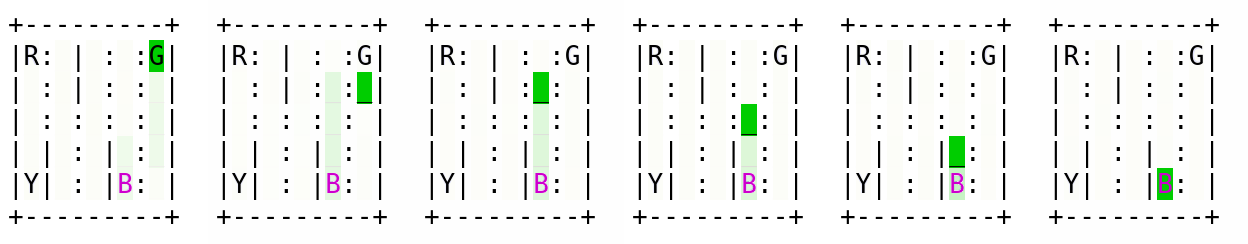
\includegraphics[width=\columnwidth]{images/merged_14_dqntaxi.png}
% 	\caption{Belief map of a Taxi driving from G to B, where the opacity describes the likelihood of the taxi entering that square as found in "What did you think would happen? Explaining Agent Behaviour through Intended Outcomes" \cite{yau2020did}}
% 	\label{fig:taxi}
% \end{figure}

\subsection{Explainable Reinforcement Learning via a Causal world model}
Explainable Reinforcement Learning via a Causal world model constructs a sparse model to connect causal relationships, without prior knowledge of the causal relationship, rather than a fully connected one, but they still achieve high accuracy and results comparable to other fully connected \ac{mbrl} policies. Which is important, as there is often a trade off between explainability and performance. Using the same model for both explanations and choosing actions also make the explanations faithful to the intentions of the agent. The paper also describes a novel approach to derive causal chains from the causal influence of the actions, which lets us find the intent of the agent. The paper is successful being applied to \ac{mbrl}, and is also applicable to models with infinite actions spaces, which is a limitation of some other models, see previous sub section.

A limitation of the paper is that it requires a known factorisation of the environment, denoted by $\langle S, A, O, R, P, T, \gamma \rangle$, where S is state space, A is action space, O is observation space, R is reward function, P is probability function for the probability of transitioning from state $s$ to state $s'$ given action $a$, T is the termination condition given the transition tuple $(s,a,o,s')$, and $\gamma$ is the discount factor. Considering we will be working with hand crafted simulations we will have access to all of these, however its not certain that if we depend on this method that our contributions will be applicable to certain other environments where the factorisation is not known.


\subsection{CrystalBox: Future-Based Explanations for Input-Driven Deep Reinforcement Learning Systems}
CrystalBox introduces a model-agnostic, post-hoc, future based explanation for \ac{drl}. It doesn't require altering the controller, and works by decomposing the future rewards into its individual components. While this isn't exactly the kind of explanation we are looking for, it could be a great tool in developing an explainer that considers other agents actions in a multi agent cooperative environment, which is the goal of our paper, because it is post-hoc, and easily deployable. Especially because it was constructed for input-driven environments. The original paper claims it offers high fidelity solutions for both discrete and continuous action spaces. KAZ has a discrete action space but we might do some work with other environments as well.

It's not certain to be useful because it works by decomposing the reward function, and it's not safe to assume the reward function will even be useful to decompose.


\subsection{Are Large Language Models Post Hoc Explainers}
A \ac{llm} is a predictive model that generates text based on a prompt you give it, be it continuing the prompt or responding, and can often give the impression of comprehension of human language and a deeper understanding of the topic at hand.  The paper aims to investigate the question "Can LLMs explain the behaviour of other complex predictive models?" by exploiting the in-context learning (ICL) capabilities of \acp{llm}. ICL allows \acp{llm} to perform well on new tasks by using a few task samples in the prompt. A benefit of using an \ac{llm} as a post-hoc explainer, is that the output given by the model will already be written in natural language and should be understandable by a layman. The paper presumes that the local behaviour of a model is a linear decision boundary, and by using a sample x and perturbing it to x', and presenting both the samples and the perturbation as natural language we could get an explanation from the \ac{llm} for the outcome. With a sufficient number of perturbations in a neighbourhood around x the \ac{llm} is expected to explain the behaviour in this neighbourhood, and rank the features in order of importance.

While the faithfulness of the \ac{llm} as an explainer is on par with other \ac{xai} methods used for classification, meaning that the reasons provided are enough to explain the output, I am sceptical of the fidelity of the \ac{llm} for two reasons. One is the same as for why other \ac{xai} models often struggle with fidelity, the temporal aspect. If applied in the same way as in the paper it would not consider the intent or the past and only what part of the current observation made it make a certain decision. The other is that I am sceptical of claims presented by an \ac{llm} in general as these are all just guesses. Good guesses a lot of the time, but still just guesses. 

We could however potentially change the implementation so it considers the temporal aspect, and this might be a viable post hoc explainer after some more research into prompt engineering.


\subsection{ACTER: Diverse and Actionable Counterfactual Sequences for Explaining and Diagnosing Reinforcement Learning Policies}
\label{sec:acter}
The paper presents ACTER, an algorithm that uses counterfactual sequences with actionable advice on how to avoid failure for an \ac{rl} policy. It does this by using an \ac{ea} known as \ac{nsga} to generate counterfactual sequences that don't lead to failure as close as possible to factual sequences that lead to failure. This paper presents counterfactual sequences and not just actions, which means it also presents how to avoid the state that lead to failure to begin with, which should, if ACTER is implemented correctly, allow us to significantly reduce the amount of times our policy fails. It also offers multiple counterfactuals to allow the end user to decide which counterfactual is preferable to their use case.

There are 4 hypothesises tested by the paper. The last two considers laymen users and are therefore not as interesting to us. The first two however "ACTER can produce counterfactual sequences that prevent failure with lower effort and higher certainty in stochastic environments compared to the baselines." and "ACTER can produce a set of counterfactual sequences that offer more diverse ways of preventing failure compared to the baselines." are partially and fully confirmed respectively. Which means ACTER will likely be a useful tool to explain and diagnose our \ac{rl} policy.


\section{Related Works}
This section describes recent development in the field of planning and future predictions. All the papers described here are directly relevant to the methods i developed.

\subsection{Predicting Future Actions Of Reinforcement Learning Agents}
\label{sec:predicting_actions}
This paper describes a method developed by the author that predicts future actions and events \cite{chung2024predictingfutureactionsreinforcement}. It does this for non planning policies, like Impala, implicit planning policies like \ac{drc}, see section \ref{sec:impl_planning}, and explicit planning policies like MuZero and Thinker.

Non planning policies are policies designed without planning in mind. Pure \ac{nn} policies without recurrency are considered to be non planning, as they have not been found to exhibit planning like behaviour. This paper found that when predicting future states and actions both inner states from implicit planners, and explicit planners improved accuracy over non planning agents.

Explicit planners are agents who simulate future states with a world model before making a decision on what action to take. They rely on the world model being accurate, and so does using them to predict future states and actions. In some environments learning an accurate world model is not feasible, an example of this is autonomous driving.

The paper proposes two methods on predicting future states and actions, simulation based and inner state based. The inner state approach is most effective when working with explicit planners, but also shows significant improvement for implicit planner agents. The simulation based approach performs very well on implicit planner agents, but requires the opportunity to train a decently performing world model. The paper also shows with an ablated world model, the inner state approach performs better.

\subsection{An Investigation of Model Free Planning}
\label{sec:impl_planning}
This paper investigates whether planning like behaviour can emerge from model free \ac{rl}, without any explicit planning methods or inductive biases designed to induce planning behaviour \cite{guez2019investigationmodelfreeplanning}. The authors introduce and explore if the \ac{drc} architecture can learn to implicitly plan through training. World models suffer from scalability issues, and inductive biases require a priori knowledge of the environment. The \ac{drc} architecture is comprised of $3$ layers of ConvLSTMs and each layer is iterated through $3$ times each at each timestep.

This architecture is tested on domains that require planning such as Sokoban, and they test the agents ability to generalize as well as data efficiency. The results of the paper is that not only does the model exhibit planning like behaviour, but it outperforms state of the art methods that use inductive biases or world models. The paper described in section \ref{sec:predicting_actions} finds that using the inner state of implicit planner agents improves predicted future states and actions.

\subsection{Stabilizing Transformers for Reinforcement Learning}


\medskip
\chapter{Methodology}

\section{Action importance}
\subsection{Counterfactual sequences}
\label{sec:counterfactual}
To discover counterfactual sequences we use the \ac{ea} known as \ac{nsga}. This algorithm is a significant improvement over earlier multi-objective EAs that use non dominated sorting. It has a complexity of $O(MN^2)$ instead of $O(MN^3)$, elitist approach and a specified sharing parameter, all three of which, many earlier algorithms lacked. \cite{Deb2001AFA} Pseudocode for sorting in algorithm \ref{alg:fnds}. 
We use multi objective search because we want to minimize action change while maximizing total reward change throughout a simulation. This defines our two objectives. This way we can discover what actions or combinations there of have the highest impact on the environment. When working with a discrete action space, that is when we have a finite, usually relatively small, amount of actions to choose from, we define the action objective that we want to minimize as how many actions in a single timestep are different from a predefined sequence found with a trained model. After the timestep with the found actions we again use the model to roll out the rest of the sequence. We compare the altered sequence to the original sequence and measure the total reward both of these sequences receive. We want to maximize this difference. See figure \ref{fig:pareto_model}. 
In the case of continuous actions we instead alter actions in multiple timesteps and use a distance measure that we want to minimize. The reward objective is similar to the case of discrete actions. See figure \ref{fig:pareto}.

\begin{algorithm}
\caption{Fast Non-Dominated Sort}
\label{alg:fnds}
\begin{algorithmic}
    \State $F_i \gets \emptyset$
    \ForAll{$p \in P$}
    \State $S_p \gets \emptyset$
    \State $n_p \gets 0$
        \ForAll{$q \in P$}
            \If{$p \prec q$}
                \State $S_p \gets S_p \cup q$
            \ElsIf{$q \prec p$}
                \State $n_p \gets n_p + 1$
            \EndIf
        \EndFor
        \If{$n_p == 0$}
            \State $F_1 \gets F_1 \cup p$
            \State $p_{rank} \gets 1$
        \EndIf
    \EndFor
    \State $i \gets 1$
    \While{$F_i \neq \emptyset$}
        \State $Q \gets \emptyset$
        \ForAll{$p \in F_i$} 
            \ForAll{$q \in S_p$}
                \State $n_q \gets n_q - 1$
                \If{$n_q \gets 0$}
                    \State $q_{rank} \gets i + 1$
                    \State $Q \gets Q \cup q$
                \EndIf
            \EndFor
        \EndFor
        \State $i \gets i + 1$
        \State $F_i \gets Q$
    \EndWhile
\end{algorithmic}
\end{algorithm}


\section{Feature importance}

\subsection{Shapley values for observations}
The Shapley value is an idea from cooperative game theory where it was used to measure the contribution of each player to the total outcome. It has been adapted to deep reinforcement learning where each feature is considered a player and the policy is considered a game. In our case we initially want to use it to explain actions so we consider that to be the outcome of the game. The Shapley value is calculated by taking each feature and finding the marginal contribution, i.e. seeing how the prediction changes when you include the feature and compare the outcome to when it wasn't included, you do this over all possible coalitions of features. See algorithm \ref{alg:shapley}.
The Shapley value has a computational complexity of $O(2^n)$, and because of this we often use estimates instead of exact Shapley values. There are two main ways of reducing the complexity. The first one is using a surrogate model instead of the policy to reduce the number of features, and the second is reducing the number of coalitions. In our case we reduce the number of coalitions to some number $2^K$ and use K-means clustering to increase representability and reduce variance.
Since we have forward passes of the policy, and each can be considered one example of a game we sample the games and use the average marginal contribution over all the games instead of just one game.
The Shapley value can help us understand how the policy acts in general. We can also use it to get explanations for single observations, however these explanations won't always have high fidelity. We will explore more of how the fidelity of Shapley values for single explanations compare to high fidelity explainability methods like gradient methods. See section \ref{sec:intgrad}

\begin{algorithm}
\caption{Shapley Value Calculation with Baseline Replacement}
\label{alg:shapley}
\begin{algorithmic}
    \State \textbf{Input:} Model $f$, input sample $x$, baseline $x'$, set of features $F$
    \State \textbf{Output:} Shapley values $\phi_f$ for each feature $f \in F$
    \State $\phi_f \gets 0 \; \forall f \in F$ \Comment{Initialize Shapley values}
    \State $n \gets |F|$ \Comment{Number of features}
    
    \ForAll{$f \in F$}
        \ForAll{$S \subseteq F \setminus \{f\}$}
            \State $x_S \gets \texttt{construct}(x, x', S)$ \Comment{Replace features not in $S$ with baseline values}
            \State $x_{S \cup \{f\}} \gets \texttt{construct}(x, x', S \cup \{f\})$
            \State $\Delta \gets f(x_{S \cup \{f\}}) - f(x_S)$ \Comment{Marginal contribution of feature $f$}
            \State $\phi_f \gets \phi_f + \frac{|S|!(n - |S| - 1)!}{n!} \Delta$
        \EndFor
    \EndFor
    \State \Return $\{\phi_f : f \in F\}$
    
    \Function{construct}{$x, x', S$}
        \State \textbf{Input:} Original sample $x$, baseline $x'$, feature subset $S$
        \State \textbf{Output:} Modified sample $x_S$
        \ForAll{$f \in F$}
            \If{$f \in S$}
                \State $x_S[f] \gets x[f]$
            \Else
                \State $x_S[f] \gets x'[f]$ \Comment{Replace with baseline value}
            \EndIf
        \EndFor
        \State \Return $x_S$
    \EndFunction
\end{algorithmic}
\end{algorithm}

\subsection{Integrated Gradients}
\label{sec:intgrad}
By integrating the gradient of the model prediction when going from a specified baseline value as input to our specific observation x we get a high fidelity explanation for what features were important in that specific observation. We integrate from the baseline instead of just getting the gradient in our observation because of the saturation problem. If a feature is important to the action the gradient could be small for the value x, but the integral of the gradient from the baseline to x would still be large. Conversely a gradient for the observation x could be significant in a small area around a feature in x even if that feature isn't as significant as the gradient in x would lead us to believe \cite{sundararajan2017axiomaticattributiondeepnetworks}. See algorithm \ref{alg:intgrad}. Comparing figure \ref{fig:intgrad} with figure \ref{fig:shap} we can see that the values are similar. This means that in the case of this observation, the fidelity of the Shapley explanation is high.

\begin{algorithm}
\caption{Integrated Gradients for Feature Importance in Reinforcement Learning}
\label{alg:intgrad}
\begin{algorithmic}
    \State \textbf{Input:} \ac{rl} policy $\pi_\theta$, input $x$, baseline input $\bar{x}$, number of steps $m$
    \State \textbf{Output:} Integrated gradients $\texttt{IG}(x, \bar{x})$
    \State $\texttt{IG}(x, \bar{x}) \gets 0 \; \forall f \in \texttt{features of } x$ \Comment{Initialize integrated gradients to zero}
    
    \For{$i = 1$ to $m$}
        \State $\alpha_i \gets \frac{i}{m}$
        \State $x_i \gets \bar{x} + \alpha_i \times (x - \bar{x})$
        \State $grad_i \gets \nabla_x \texttt{value}(\pi_\theta, x_i)$ \Comment{Compute the gradient of the value function}
        \State $\texttt{IG}(x, \bar{x}) \gets \texttt{IG}(x, \bar{x}) + grad_i \times \frac{(x - \bar{x})}{m}$
        \Comment{Accumulate gradients scaled by the step size}
    \EndFor
    
    \Function{value}{$\pi_\theta, x$}
        \State \textbf{Input:} \ac{rl} policy $\pi_\theta$, input $x$
        \State \textbf{Output:} Model prediction for input $x$
        
        \State $\texttt{Feed input } x \texttt{ to policy } \pi_\theta$
        \State \Return \texttt{model output}
    \EndFunction
\end{algorithmic}
\end{algorithm}


\subsection{Choosing a baseline}

\section{Extracting intent}

In an environment where the agents successfully reaches a desirable state we can assume that at some point in the trajectory an agents intent is to reach this state. We can train a prediction model on such an environment that uses a certain state or observation as input and outputs features of interest some time in the future. In the example of autonomous vehicles the output could be predicted position of the vehicle at a future point in time. If our prediction model is successful, then it could be considered part of an explanation for the intent of an agent.
Additionally, we train different models with different sets of inputs to identify what is important to identify intent. We train one model that takes just the observation as input, one that takes observation and action, and one that takes observation and action one hot encoded. While action as an integer and action one hot encoded contains the same amount of information it could be easier for a network to learn correlations with the additional inputs. Looking at the loss curve during training, as well as final loss, this suspicion is confirmed to be true when dealing with a network architecture and environment like we are currently using, 2 fully connected hidden layers with the hyperbolic tangent as the activation, in the environment simple\_spread\_v3. While the input layer for the three prediction models are slightly different the difference in training time is negligible. 
After 200 epochs the base prediction model reached a evaluation loss of 0.0407, the model with integer action as part of the input reached a evaluation loss of 0.0359 and the model with one-hot encoded action as part of the input reached an evaluation loss of 0.0322. See figure \ref{fig:pred_loss_none}, \ref{fig:pred_loss_action} and \ref{fig:pred_loss_one-hot}. Both the base model and the one-hot action model stagnate long before 200 epochs is reached. If we let the model with integer action as input train for another 50 epochs it does not improve. The test loss for these three models respectively is ... . These graphs and values indicate that while action and an explanation are useful for extracting intent, in the context of our environment and model one-hot values and integrated gradient explanation are the most useful. The difference between using Shapley values and


\section{LSTM values}
An \ac{lstm} cell takes as input a cell state $c_{t-1}$, a hidden state $h_{t-1}$, and an input $X_t$ for each timestep. It outputs a cell state $c_{t}$, a hidden state $h_{t}$ and an output $y_t$. $h_{t-1}$ is concatenated with $X_t$ and then with trainable weight matrices $\textbf{W}$ and biases $b$, $c_t$ and $h_t$ are computed according to the following equations:

\[
f_t = \sigma(W_f [h_{t-1}, x_t] + b_f)
\]

\[
i_t = \sigma(W_i [h_{t-1}, x_t] + b_i)
\]

\[
\tilde{c}_t = \tanh(W_c [h_{t-1}, x_t] + b_c)
\]

\[
c_t = f_t \odot c_{t-1} + i_t \odot \tilde{c}_t
\]

\[
o_t = \sigma(W_o [h_{t-1}, x_t] + b_o)
\]

\[
h_t = o_t \odot \tanh(c_t)
\]

Intuitively, $f_t$ can be viewed as how much of the previous cell state $c_{t-1}$ to forget, $i_t$ can be viewed as how much of the candidate cell state $\tilde{c}_t$ to remember, and $o_t$ can be viewed as how much of the $c_{t}$ to output. Capital letters represent matrices and lowercase letters represent vectors.

\begin{center}
\begin{figure}
\begin{tikzpicture}[>=Stealth, node distance=1.5cm, auto]
\hspace{4cm}
  % LSTM cell as a pastel purple box with rounded corners
  \node[draw, fill=purple!30, rounded corners, minimum width=3cm, minimum height=2cm] (lstm) {LSTM};

  % Incoming arrows on the left: previous cell state (c) and hidden state (h)
  \draw[<-] ([yshift=0.3cm]lstm.west) -- ++(-1,0) node[left] {\(c_{t-1}\)};
  \draw[<-] ([yshift=-0.3cm]lstm.west) -- ++(-1,0) node[left] {\(h_{t-1}\)};

  % Outgoing arrows on the right: new cell state (c) and hidden state (h)
  \draw[->] ([yshift=0.3cm]lstm.east) -- ++(1,0) node[right] {\(c_t\)};
  \draw[->] ([yshift=-0.3cm]lstm.east) -- ++(1,0) node[right] {\(h_t\)};

  \draw[<-] (lstm.south) -- ++(0,-1) node[below] {\(x_t\)};
  \draw[->] (lstm.north) -- ++(0,1) node[above] {\(h_t\)};
\end{tikzpicture}
\caption{Simplified illustration of an \ac{lstm} layer}
\label{fig:lstm}
\end{figure}
\end{center}

As $c_t$ and $h_t$ are helpful when predicting future actions and states \cite{chung2024predictingfutureactionsreinforcement} when considering the \ac{drc} architecture, I hypothesize that the same holds when using a regular \ac{lstm} layer. See figure \ref{fig:lstm}.



\chapter{Experiments}
\section{General experimental setup}
I have several \acp{nn} for each experiment. The goal is to train them to predict states and events. For the state prediction I initially trained a \ac{nn}, $state_{base}$ to take the observations made by a type of agent from step $n$, $Obs_n$, and output the $x$ and $y$ coordinates of the same agent at step $n+m$ in a trajectory. The dataset $D_pos$ was constructed such that each data point was from a different trajectory $\tau$, to make sure all the data points were independent of each other, in order to make sure the \ac{nn} did not learn any such connection. The variable $n$ was chosen randomly for each trajectory while $m$ stayed as a constant, in my case $m=10$. I would for example have $50000$ trajectories, each trajectory contains $2$ archers, so we would have a dataset of size $100000$. $100000$ observations and their corresponding positions $10$ steps into the future. We assume that both archers use the same policy as they are homogeneous.

I also trained a \ac{nn} for event prediction, $event_{base}$. The event we trained a network to predict was whether an agent would encounter a critical state or not. See section placeholder. The dataset $D_{crit}$ was similar to $D_{pos}$, however instead of positions, it would contain whether the agent would encounter a critical state within the next $5$ steps. 

I consider the accuracy of $event_{base}$ and the average error measured in euclidean distance of $state_{base}$ to be the baselines i compare results against in the first experiment. I will train other neural networks.

The \ac{nn} was a fully connected network, had two hidden layers of size 64 each and used the activation function $tanh$. This neural network got an accuracy of $0.8244$ on the test set and the average distance from target was $0.0409$ on the test set. This \ac{nn} is purely a post hoc explainer and used no information about the policy what so ever to explain the agents intention. As aforementioned we want to include information about the policy to discover how we can improve this prediction, and better discover the intent of the agent.

All hyper parameters stayed the same. Only The dataset, and therefore also the input layer, was different between the runs. I trained the networks for a total of $200$ epochs, after which improvement was negligible, if at all existent, with a learning rate scheduler that decreased learning rate when loss reached a plateau, which was measured on a validation set.

I decided to reject all results that showed a relative change of less than $2\%$ when compared to the baseline, as \acp{nn} will always be approximations of the optimal distribution achievable when considering a specific dataset, which means that even in the case of new input having no relevant information we will get some variation in the results. An improvement of $2\%$ or less is not an improvement worth the cost in most scenarios.

\section{Action and explanation inclusion}
\subsection{Setup}
I enhanced both the dataset $D_{pos}$ and $D_{crit}$ with a series of other data. For both datasets I included the action, encoded by an integer from $0$ to $n_{acts}$, i.e. the amount of actions an agent has available, taken at $Obs_n$ for each data point, to use as input for an \ac{nn}. I then trained two \acp{nn} with the same architecture as $state_{base}$ and $event_{base}$ respectively, and once again measured accuracy for the event predictor net with included action, and average error for the state predictor net with included action. If the predictions improved I considered the action to be useful on its own for the predictions in the given environment.

I then one-hot encoded the action, i.e. encoded the action as a $n_{acts}$ dimensional unit vector with a 1 in the chosen action dimension. This includes the same amount of information as represented as an integer, however I hypothesized that the resulting network would achieve higher performance with one-hot encoded actions as the distance between independent actions when one-hot encoding the actions are all the same, as opposed to when encoding the actions as an integer when the distance between two actions is not constant. For example, between the action encoded as the integer 2 and the action encoded as the integer 3 the Manhattan distance is 1, but between the action encoded as the integer 2 and the action encoded as the integer 4 the Manhattan distance is 2. When one-hot encoding these actions the Manhattan distance between two distinct actions will in all cases be 2. As in the previous cases I also trained a \ac{nn} on the datasets enhanced with one hot encoded actions.

After creating datasets with actions encoded different ways I also created two feature importance explanations for the action chosen in each of the initial observations. Shapley values and Integrated gradients were the two methods chosen. I decided on 2 feature importance measures that internally uses different methods of calculation, gradients and SHAP, to explore if they would yield different results. The motivation behind including feature importance explanations is that it describes some if the inner processing of the policy, and might therefore elucidate what kind of actions it might take in future states, and therefore include some of the intent. On each of the previous datasets I created new datasets with these two feature importance methods included.

In total I trained 18 neural networks per environment, one for each dataset constructed, and compared the results for accuracy on the event prediction networks and the results for average error on the state prediction networks. I repeated this experiment for a few different environments to explore if the results vary depending on environment.
\begin{figure}[!ht]
	%% Creator: Matplotlib, PGF backend
%%
%% To include the figure in your LaTeX document, write
%%   \input{<filename>.pgf}
%%
%% Make sure the required packages are loaded in your preamble
%%   \usepackage{pgf}
%%
%% Also ensure that all the required font packages are loaded; for instance,
%% the lmodern package is sometimes necessary when using math font.
%%   \usepackage{lmodern}
%%
%% Figures using additional raster images can only be included by \input if
%% they are in the same directory as the main LaTeX file. For loading figures
%% from other directories you can use the `import` package
%%   \usepackage{import}
%%
%% and then include the figures with
%%   \import{<path to file>}{<filename>.pgf}
%%
%% Matplotlib used the following preamble
%%   \def\mathdefault#1{#1}
%%   \everymath=\expandafter{\the\everymath\displaystyle}
%%   \IfFileExists{scrextend.sty}{
%%     \usepackage[fontsize=10.000000pt]{scrextend}
%%   }{
%%     \renewcommand{\normalsize}{\fontsize{10.000000}{12.000000}\selectfont}
%%     \normalsize
%%   }
%%   
%%   \ifdefined\pdftexversion\else  % non-pdftex case.
%%     \usepackage{fontspec}
%%     \setmainfont{DejaVuSerif.ttf}[Path=\detokenize{/uio/hume/student-u79/adaha/master_thesis/.venv/lib/python3.11/site-packages/matplotlib/mpl-data/fonts/ttf/}]
%%     \setsansfont{DejaVuSans.ttf}[Path=\detokenize{/uio/hume/student-u79/adaha/master_thesis/.venv/lib/python3.11/site-packages/matplotlib/mpl-data/fonts/ttf/}]
%%     \setmonofont{DejaVuSansMono.ttf}[Path=\detokenize{/uio/hume/student-u79/adaha/master_thesis/.venv/lib/python3.11/site-packages/matplotlib/mpl-data/fonts/ttf/}]
%%   \fi
%%   \makeatletter\@ifpackageloaded{underscore}{}{\usepackage[strings]{underscore}}\makeatother
%%
\begingroup%
\makeatletter%
\begin{pgfpicture}%
\pgfpathrectangle{\pgfpointorigin}{\pgfqpoint{6.400000in}{4.800000in}}%
\pgfusepath{use as bounding box, clip}%
\begin{pgfscope}%
\pgfsetbuttcap%
\pgfsetmiterjoin%
\definecolor{currentfill}{rgb}{1.000000,1.000000,1.000000}%
\pgfsetfillcolor{currentfill}%
\pgfsetlinewidth{0.000000pt}%
\definecolor{currentstroke}{rgb}{1.000000,1.000000,1.000000}%
\pgfsetstrokecolor{currentstroke}%
\pgfsetdash{}{0pt}%
\pgfpathmoveto{\pgfqpoint{0.000000in}{0.000000in}}%
\pgfpathlineto{\pgfqpoint{6.400000in}{0.000000in}}%
\pgfpathlineto{\pgfqpoint{6.400000in}{4.800000in}}%
\pgfpathlineto{\pgfqpoint{0.000000in}{4.800000in}}%
\pgfpathlineto{\pgfqpoint{0.000000in}{0.000000in}}%
\pgfpathclose%
\pgfusepath{fill}%
\end{pgfscope}%
\begin{pgfscope}%
\pgfsetbuttcap%
\pgfsetmiterjoin%
\definecolor{currentfill}{rgb}{1.000000,1.000000,1.000000}%
\pgfsetfillcolor{currentfill}%
\pgfsetlinewidth{0.000000pt}%
\definecolor{currentstroke}{rgb}{0.000000,0.000000,0.000000}%
\pgfsetstrokecolor{currentstroke}%
\pgfsetstrokeopacity{0.000000}%
\pgfsetdash{}{0pt}%
\pgfpathmoveto{\pgfqpoint{0.800000in}{0.528000in}}%
\pgfpathlineto{\pgfqpoint{5.760000in}{0.528000in}}%
\pgfpathlineto{\pgfqpoint{5.760000in}{4.224000in}}%
\pgfpathlineto{\pgfqpoint{0.800000in}{4.224000in}}%
\pgfpathlineto{\pgfqpoint{0.800000in}{0.528000in}}%
\pgfpathclose%
\pgfusepath{fill}%
\end{pgfscope}%
\begin{pgfscope}%
\pgfsetbuttcap%
\pgfsetroundjoin%
\definecolor{currentfill}{rgb}{0.000000,0.000000,0.000000}%
\pgfsetfillcolor{currentfill}%
\pgfsetlinewidth{0.803000pt}%
\definecolor{currentstroke}{rgb}{0.000000,0.000000,0.000000}%
\pgfsetstrokecolor{currentstroke}%
\pgfsetdash{}{0pt}%
\pgfsys@defobject{currentmarker}{\pgfqpoint{0.000000in}{-0.048611in}}{\pgfqpoint{0.000000in}{0.000000in}}{%
\pgfpathmoveto{\pgfqpoint{0.000000in}{0.000000in}}%
\pgfpathlineto{\pgfqpoint{0.000000in}{-0.048611in}}%
\pgfusepath{stroke,fill}%
}%
\begin{pgfscope}%
\pgfsys@transformshift{1.002796in}{0.528000in}%
\pgfsys@useobject{currentmarker}{}%
\end{pgfscope}%
\end{pgfscope}%
\begin{pgfscope}%
\definecolor{textcolor}{rgb}{0.000000,0.000000,0.000000}%
\pgfsetstrokecolor{textcolor}%
\pgfsetfillcolor{textcolor}%
\pgftext[x=1.002796in,y=0.430778in,,top]{\color{textcolor}{\sffamily\fontsize{10.000000}{12.000000}\selectfont\catcode`\^=\active\def^{\ifmmode\sp\else\^{}\fi}\catcode`\%=\active\def%{\%}0}}%
\end{pgfscope}%
\begin{pgfscope}%
\pgfsetbuttcap%
\pgfsetroundjoin%
\definecolor{currentfill}{rgb}{0.000000,0.000000,0.000000}%
\pgfsetfillcolor{currentfill}%
\pgfsetlinewidth{0.803000pt}%
\definecolor{currentstroke}{rgb}{0.000000,0.000000,0.000000}%
\pgfsetstrokecolor{currentstroke}%
\pgfsetdash{}{0pt}%
\pgfsys@defobject{currentmarker}{\pgfqpoint{0.000000in}{-0.048611in}}{\pgfqpoint{0.000000in}{0.000000in}}{%
\pgfpathmoveto{\pgfqpoint{0.000000in}{0.000000in}}%
\pgfpathlineto{\pgfqpoint{0.000000in}{-0.048611in}}%
\pgfusepath{stroke,fill}%
}%
\begin{pgfscope}%
\pgfsys@transformshift{1.569265in}{0.528000in}%
\pgfsys@useobject{currentmarker}{}%
\end{pgfscope}%
\end{pgfscope}%
\begin{pgfscope}%
\definecolor{textcolor}{rgb}{0.000000,0.000000,0.000000}%
\pgfsetstrokecolor{textcolor}%
\pgfsetfillcolor{textcolor}%
\pgftext[x=1.569265in,y=0.430778in,,top]{\color{textcolor}{\sffamily\fontsize{10.000000}{12.000000}\selectfont\catcode`\^=\active\def^{\ifmmode\sp\else\^{}\fi}\catcode`\%=\active\def%{\%}25}}%
\end{pgfscope}%
\begin{pgfscope}%
\pgfsetbuttcap%
\pgfsetroundjoin%
\definecolor{currentfill}{rgb}{0.000000,0.000000,0.000000}%
\pgfsetfillcolor{currentfill}%
\pgfsetlinewidth{0.803000pt}%
\definecolor{currentstroke}{rgb}{0.000000,0.000000,0.000000}%
\pgfsetstrokecolor{currentstroke}%
\pgfsetdash{}{0pt}%
\pgfsys@defobject{currentmarker}{\pgfqpoint{0.000000in}{-0.048611in}}{\pgfqpoint{0.000000in}{0.000000in}}{%
\pgfpathmoveto{\pgfqpoint{0.000000in}{0.000000in}}%
\pgfpathlineto{\pgfqpoint{0.000000in}{-0.048611in}}%
\pgfusepath{stroke,fill}%
}%
\begin{pgfscope}%
\pgfsys@transformshift{2.135733in}{0.528000in}%
\pgfsys@useobject{currentmarker}{}%
\end{pgfscope}%
\end{pgfscope}%
\begin{pgfscope}%
\definecolor{textcolor}{rgb}{0.000000,0.000000,0.000000}%
\pgfsetstrokecolor{textcolor}%
\pgfsetfillcolor{textcolor}%
\pgftext[x=2.135733in,y=0.430778in,,top]{\color{textcolor}{\sffamily\fontsize{10.000000}{12.000000}\selectfont\catcode`\^=\active\def^{\ifmmode\sp\else\^{}\fi}\catcode`\%=\active\def%{\%}50}}%
\end{pgfscope}%
\begin{pgfscope}%
\pgfsetbuttcap%
\pgfsetroundjoin%
\definecolor{currentfill}{rgb}{0.000000,0.000000,0.000000}%
\pgfsetfillcolor{currentfill}%
\pgfsetlinewidth{0.803000pt}%
\definecolor{currentstroke}{rgb}{0.000000,0.000000,0.000000}%
\pgfsetstrokecolor{currentstroke}%
\pgfsetdash{}{0pt}%
\pgfsys@defobject{currentmarker}{\pgfqpoint{0.000000in}{-0.048611in}}{\pgfqpoint{0.000000in}{0.000000in}}{%
\pgfpathmoveto{\pgfqpoint{0.000000in}{0.000000in}}%
\pgfpathlineto{\pgfqpoint{0.000000in}{-0.048611in}}%
\pgfusepath{stroke,fill}%
}%
\begin{pgfscope}%
\pgfsys@transformshift{2.702202in}{0.528000in}%
\pgfsys@useobject{currentmarker}{}%
\end{pgfscope}%
\end{pgfscope}%
\begin{pgfscope}%
\definecolor{textcolor}{rgb}{0.000000,0.000000,0.000000}%
\pgfsetstrokecolor{textcolor}%
\pgfsetfillcolor{textcolor}%
\pgftext[x=2.702202in,y=0.430778in,,top]{\color{textcolor}{\sffamily\fontsize{10.000000}{12.000000}\selectfont\catcode`\^=\active\def^{\ifmmode\sp\else\^{}\fi}\catcode`\%=\active\def%{\%}75}}%
\end{pgfscope}%
\begin{pgfscope}%
\pgfsetbuttcap%
\pgfsetroundjoin%
\definecolor{currentfill}{rgb}{0.000000,0.000000,0.000000}%
\pgfsetfillcolor{currentfill}%
\pgfsetlinewidth{0.803000pt}%
\definecolor{currentstroke}{rgb}{0.000000,0.000000,0.000000}%
\pgfsetstrokecolor{currentstroke}%
\pgfsetdash{}{0pt}%
\pgfsys@defobject{currentmarker}{\pgfqpoint{0.000000in}{-0.048611in}}{\pgfqpoint{0.000000in}{0.000000in}}{%
\pgfpathmoveto{\pgfqpoint{0.000000in}{0.000000in}}%
\pgfpathlineto{\pgfqpoint{0.000000in}{-0.048611in}}%
\pgfusepath{stroke,fill}%
}%
\begin{pgfscope}%
\pgfsys@transformshift{3.268671in}{0.528000in}%
\pgfsys@useobject{currentmarker}{}%
\end{pgfscope}%
\end{pgfscope}%
\begin{pgfscope}%
\definecolor{textcolor}{rgb}{0.000000,0.000000,0.000000}%
\pgfsetstrokecolor{textcolor}%
\pgfsetfillcolor{textcolor}%
\pgftext[x=3.268671in,y=0.430778in,,top]{\color{textcolor}{\sffamily\fontsize{10.000000}{12.000000}\selectfont\catcode`\^=\active\def^{\ifmmode\sp\else\^{}\fi}\catcode`\%=\active\def%{\%}100}}%
\end{pgfscope}%
\begin{pgfscope}%
\pgfsetbuttcap%
\pgfsetroundjoin%
\definecolor{currentfill}{rgb}{0.000000,0.000000,0.000000}%
\pgfsetfillcolor{currentfill}%
\pgfsetlinewidth{0.803000pt}%
\definecolor{currentstroke}{rgb}{0.000000,0.000000,0.000000}%
\pgfsetstrokecolor{currentstroke}%
\pgfsetdash{}{0pt}%
\pgfsys@defobject{currentmarker}{\pgfqpoint{0.000000in}{-0.048611in}}{\pgfqpoint{0.000000in}{0.000000in}}{%
\pgfpathmoveto{\pgfqpoint{0.000000in}{0.000000in}}%
\pgfpathlineto{\pgfqpoint{0.000000in}{-0.048611in}}%
\pgfusepath{stroke,fill}%
}%
\begin{pgfscope}%
\pgfsys@transformshift{3.835139in}{0.528000in}%
\pgfsys@useobject{currentmarker}{}%
\end{pgfscope}%
\end{pgfscope}%
\begin{pgfscope}%
\definecolor{textcolor}{rgb}{0.000000,0.000000,0.000000}%
\pgfsetstrokecolor{textcolor}%
\pgfsetfillcolor{textcolor}%
\pgftext[x=3.835139in,y=0.430778in,,top]{\color{textcolor}{\sffamily\fontsize{10.000000}{12.000000}\selectfont\catcode`\^=\active\def^{\ifmmode\sp\else\^{}\fi}\catcode`\%=\active\def%{\%}125}}%
\end{pgfscope}%
\begin{pgfscope}%
\pgfsetbuttcap%
\pgfsetroundjoin%
\definecolor{currentfill}{rgb}{0.000000,0.000000,0.000000}%
\pgfsetfillcolor{currentfill}%
\pgfsetlinewidth{0.803000pt}%
\definecolor{currentstroke}{rgb}{0.000000,0.000000,0.000000}%
\pgfsetstrokecolor{currentstroke}%
\pgfsetdash{}{0pt}%
\pgfsys@defobject{currentmarker}{\pgfqpoint{0.000000in}{-0.048611in}}{\pgfqpoint{0.000000in}{0.000000in}}{%
\pgfpathmoveto{\pgfqpoint{0.000000in}{0.000000in}}%
\pgfpathlineto{\pgfqpoint{0.000000in}{-0.048611in}}%
\pgfusepath{stroke,fill}%
}%
\begin{pgfscope}%
\pgfsys@transformshift{4.401608in}{0.528000in}%
\pgfsys@useobject{currentmarker}{}%
\end{pgfscope}%
\end{pgfscope}%
\begin{pgfscope}%
\definecolor{textcolor}{rgb}{0.000000,0.000000,0.000000}%
\pgfsetstrokecolor{textcolor}%
\pgfsetfillcolor{textcolor}%
\pgftext[x=4.401608in,y=0.430778in,,top]{\color{textcolor}{\sffamily\fontsize{10.000000}{12.000000}\selectfont\catcode`\^=\active\def^{\ifmmode\sp\else\^{}\fi}\catcode`\%=\active\def%{\%}150}}%
\end{pgfscope}%
\begin{pgfscope}%
\pgfsetbuttcap%
\pgfsetroundjoin%
\definecolor{currentfill}{rgb}{0.000000,0.000000,0.000000}%
\pgfsetfillcolor{currentfill}%
\pgfsetlinewidth{0.803000pt}%
\definecolor{currentstroke}{rgb}{0.000000,0.000000,0.000000}%
\pgfsetstrokecolor{currentstroke}%
\pgfsetdash{}{0pt}%
\pgfsys@defobject{currentmarker}{\pgfqpoint{0.000000in}{-0.048611in}}{\pgfqpoint{0.000000in}{0.000000in}}{%
\pgfpathmoveto{\pgfqpoint{0.000000in}{0.000000in}}%
\pgfpathlineto{\pgfqpoint{0.000000in}{-0.048611in}}%
\pgfusepath{stroke,fill}%
}%
\begin{pgfscope}%
\pgfsys@transformshift{4.968077in}{0.528000in}%
\pgfsys@useobject{currentmarker}{}%
\end{pgfscope}%
\end{pgfscope}%
\begin{pgfscope}%
\definecolor{textcolor}{rgb}{0.000000,0.000000,0.000000}%
\pgfsetstrokecolor{textcolor}%
\pgfsetfillcolor{textcolor}%
\pgftext[x=4.968077in,y=0.430778in,,top]{\color{textcolor}{\sffamily\fontsize{10.000000}{12.000000}\selectfont\catcode`\^=\active\def^{\ifmmode\sp\else\^{}\fi}\catcode`\%=\active\def%{\%}175}}%
\end{pgfscope}%
\begin{pgfscope}%
\pgfsetbuttcap%
\pgfsetroundjoin%
\definecolor{currentfill}{rgb}{0.000000,0.000000,0.000000}%
\pgfsetfillcolor{currentfill}%
\pgfsetlinewidth{0.803000pt}%
\definecolor{currentstroke}{rgb}{0.000000,0.000000,0.000000}%
\pgfsetstrokecolor{currentstroke}%
\pgfsetdash{}{0pt}%
\pgfsys@defobject{currentmarker}{\pgfqpoint{0.000000in}{-0.048611in}}{\pgfqpoint{0.000000in}{0.000000in}}{%
\pgfpathmoveto{\pgfqpoint{0.000000in}{0.000000in}}%
\pgfpathlineto{\pgfqpoint{0.000000in}{-0.048611in}}%
\pgfusepath{stroke,fill}%
}%
\begin{pgfscope}%
\pgfsys@transformshift{5.534545in}{0.528000in}%
\pgfsys@useobject{currentmarker}{}%
\end{pgfscope}%
\end{pgfscope}%
\begin{pgfscope}%
\definecolor{textcolor}{rgb}{0.000000,0.000000,0.000000}%
\pgfsetstrokecolor{textcolor}%
\pgfsetfillcolor{textcolor}%
\pgftext[x=5.534545in,y=0.430778in,,top]{\color{textcolor}{\sffamily\fontsize{10.000000}{12.000000}\selectfont\catcode`\^=\active\def^{\ifmmode\sp\else\^{}\fi}\catcode`\%=\active\def%{\%}200}}%
\end{pgfscope}%
\begin{pgfscope}%
\definecolor{textcolor}{rgb}{0.000000,0.000000,0.000000}%
\pgfsetstrokecolor{textcolor}%
\pgfsetfillcolor{textcolor}%
\pgftext[x=3.280000in,y=0.240809in,,top]{\color{textcolor}{\sffamily\fontsize{10.000000}{12.000000}\selectfont\catcode`\^=\active\def^{\ifmmode\sp\else\^{}\fi}\catcode`\%=\active\def%{\%}Epoch}}%
\end{pgfscope}%
\begin{pgfscope}%
\pgfsetbuttcap%
\pgfsetroundjoin%
\definecolor{currentfill}{rgb}{0.000000,0.000000,0.000000}%
\pgfsetfillcolor{currentfill}%
\pgfsetlinewidth{0.803000pt}%
\definecolor{currentstroke}{rgb}{0.000000,0.000000,0.000000}%
\pgfsetstrokecolor{currentstroke}%
\pgfsetdash{}{0pt}%
\pgfsys@defobject{currentmarker}{\pgfqpoint{-0.048611in}{0.000000in}}{\pgfqpoint{-0.000000in}{0.000000in}}{%
\pgfpathmoveto{\pgfqpoint{-0.000000in}{0.000000in}}%
\pgfpathlineto{\pgfqpoint{-0.048611in}{0.000000in}}%
\pgfusepath{stroke,fill}%
}%
\begin{pgfscope}%
\pgfsys@transformshift{0.800000in}{0.833856in}%
\pgfsys@useobject{currentmarker}{}%
\end{pgfscope}%
\end{pgfscope}%
\begin{pgfscope}%
\definecolor{textcolor}{rgb}{0.000000,0.000000,0.000000}%
\pgfsetstrokecolor{textcolor}%
\pgfsetfillcolor{textcolor}%
\pgftext[x=0.393533in, y=0.781094in, left, base]{\color{textcolor}{\sffamily\fontsize{10.000000}{12.000000}\selectfont\catcode`\^=\active\def^{\ifmmode\sp\else\^{}\fi}\catcode`\%=\active\def%{\%}0.40}}%
\end{pgfscope}%
\begin{pgfscope}%
\pgfsetbuttcap%
\pgfsetroundjoin%
\definecolor{currentfill}{rgb}{0.000000,0.000000,0.000000}%
\pgfsetfillcolor{currentfill}%
\pgfsetlinewidth{0.803000pt}%
\definecolor{currentstroke}{rgb}{0.000000,0.000000,0.000000}%
\pgfsetstrokecolor{currentstroke}%
\pgfsetdash{}{0pt}%
\pgfsys@defobject{currentmarker}{\pgfqpoint{-0.048611in}{0.000000in}}{\pgfqpoint{-0.000000in}{0.000000in}}{%
\pgfpathmoveto{\pgfqpoint{-0.000000in}{0.000000in}}%
\pgfpathlineto{\pgfqpoint{-0.048611in}{0.000000in}}%
\pgfusepath{stroke,fill}%
}%
\begin{pgfscope}%
\pgfsys@transformshift{0.800000in}{1.384119in}%
\pgfsys@useobject{currentmarker}{}%
\end{pgfscope}%
\end{pgfscope}%
\begin{pgfscope}%
\definecolor{textcolor}{rgb}{0.000000,0.000000,0.000000}%
\pgfsetstrokecolor{textcolor}%
\pgfsetfillcolor{textcolor}%
\pgftext[x=0.393533in, y=1.331357in, left, base]{\color{textcolor}{\sffamily\fontsize{10.000000}{12.000000}\selectfont\catcode`\^=\active\def^{\ifmmode\sp\else\^{}\fi}\catcode`\%=\active\def%{\%}0.45}}%
\end{pgfscope}%
\begin{pgfscope}%
\pgfsetbuttcap%
\pgfsetroundjoin%
\definecolor{currentfill}{rgb}{0.000000,0.000000,0.000000}%
\pgfsetfillcolor{currentfill}%
\pgfsetlinewidth{0.803000pt}%
\definecolor{currentstroke}{rgb}{0.000000,0.000000,0.000000}%
\pgfsetstrokecolor{currentstroke}%
\pgfsetdash{}{0pt}%
\pgfsys@defobject{currentmarker}{\pgfqpoint{-0.048611in}{0.000000in}}{\pgfqpoint{-0.000000in}{0.000000in}}{%
\pgfpathmoveto{\pgfqpoint{-0.000000in}{0.000000in}}%
\pgfpathlineto{\pgfqpoint{-0.048611in}{0.000000in}}%
\pgfusepath{stroke,fill}%
}%
\begin{pgfscope}%
\pgfsys@transformshift{0.800000in}{1.934382in}%
\pgfsys@useobject{currentmarker}{}%
\end{pgfscope}%
\end{pgfscope}%
\begin{pgfscope}%
\definecolor{textcolor}{rgb}{0.000000,0.000000,0.000000}%
\pgfsetstrokecolor{textcolor}%
\pgfsetfillcolor{textcolor}%
\pgftext[x=0.393533in, y=1.881620in, left, base]{\color{textcolor}{\sffamily\fontsize{10.000000}{12.000000}\selectfont\catcode`\^=\active\def^{\ifmmode\sp\else\^{}\fi}\catcode`\%=\active\def%{\%}0.50}}%
\end{pgfscope}%
\begin{pgfscope}%
\pgfsetbuttcap%
\pgfsetroundjoin%
\definecolor{currentfill}{rgb}{0.000000,0.000000,0.000000}%
\pgfsetfillcolor{currentfill}%
\pgfsetlinewidth{0.803000pt}%
\definecolor{currentstroke}{rgb}{0.000000,0.000000,0.000000}%
\pgfsetstrokecolor{currentstroke}%
\pgfsetdash{}{0pt}%
\pgfsys@defobject{currentmarker}{\pgfqpoint{-0.048611in}{0.000000in}}{\pgfqpoint{-0.000000in}{0.000000in}}{%
\pgfpathmoveto{\pgfqpoint{-0.000000in}{0.000000in}}%
\pgfpathlineto{\pgfqpoint{-0.048611in}{0.000000in}}%
\pgfusepath{stroke,fill}%
}%
\begin{pgfscope}%
\pgfsys@transformshift{0.800000in}{2.484645in}%
\pgfsys@useobject{currentmarker}{}%
\end{pgfscope}%
\end{pgfscope}%
\begin{pgfscope}%
\definecolor{textcolor}{rgb}{0.000000,0.000000,0.000000}%
\pgfsetstrokecolor{textcolor}%
\pgfsetfillcolor{textcolor}%
\pgftext[x=0.393533in, y=2.431883in, left, base]{\color{textcolor}{\sffamily\fontsize{10.000000}{12.000000}\selectfont\catcode`\^=\active\def^{\ifmmode\sp\else\^{}\fi}\catcode`\%=\active\def%{\%}0.55}}%
\end{pgfscope}%
\begin{pgfscope}%
\pgfsetbuttcap%
\pgfsetroundjoin%
\definecolor{currentfill}{rgb}{0.000000,0.000000,0.000000}%
\pgfsetfillcolor{currentfill}%
\pgfsetlinewidth{0.803000pt}%
\definecolor{currentstroke}{rgb}{0.000000,0.000000,0.000000}%
\pgfsetstrokecolor{currentstroke}%
\pgfsetdash{}{0pt}%
\pgfsys@defobject{currentmarker}{\pgfqpoint{-0.048611in}{0.000000in}}{\pgfqpoint{-0.000000in}{0.000000in}}{%
\pgfpathmoveto{\pgfqpoint{-0.000000in}{0.000000in}}%
\pgfpathlineto{\pgfqpoint{-0.048611in}{0.000000in}}%
\pgfusepath{stroke,fill}%
}%
\begin{pgfscope}%
\pgfsys@transformshift{0.800000in}{3.034908in}%
\pgfsys@useobject{currentmarker}{}%
\end{pgfscope}%
\end{pgfscope}%
\begin{pgfscope}%
\definecolor{textcolor}{rgb}{0.000000,0.000000,0.000000}%
\pgfsetstrokecolor{textcolor}%
\pgfsetfillcolor{textcolor}%
\pgftext[x=0.393533in, y=2.982147in, left, base]{\color{textcolor}{\sffamily\fontsize{10.000000}{12.000000}\selectfont\catcode`\^=\active\def^{\ifmmode\sp\else\^{}\fi}\catcode`\%=\active\def%{\%}0.60}}%
\end{pgfscope}%
\begin{pgfscope}%
\pgfsetbuttcap%
\pgfsetroundjoin%
\definecolor{currentfill}{rgb}{0.000000,0.000000,0.000000}%
\pgfsetfillcolor{currentfill}%
\pgfsetlinewidth{0.803000pt}%
\definecolor{currentstroke}{rgb}{0.000000,0.000000,0.000000}%
\pgfsetstrokecolor{currentstroke}%
\pgfsetdash{}{0pt}%
\pgfsys@defobject{currentmarker}{\pgfqpoint{-0.048611in}{0.000000in}}{\pgfqpoint{-0.000000in}{0.000000in}}{%
\pgfpathmoveto{\pgfqpoint{-0.000000in}{0.000000in}}%
\pgfpathlineto{\pgfqpoint{-0.048611in}{0.000000in}}%
\pgfusepath{stroke,fill}%
}%
\begin{pgfscope}%
\pgfsys@transformshift{0.800000in}{3.585171in}%
\pgfsys@useobject{currentmarker}{}%
\end{pgfscope}%
\end{pgfscope}%
\begin{pgfscope}%
\definecolor{textcolor}{rgb}{0.000000,0.000000,0.000000}%
\pgfsetstrokecolor{textcolor}%
\pgfsetfillcolor{textcolor}%
\pgftext[x=0.393533in, y=3.532410in, left, base]{\color{textcolor}{\sffamily\fontsize{10.000000}{12.000000}\selectfont\catcode`\^=\active\def^{\ifmmode\sp\else\^{}\fi}\catcode`\%=\active\def%{\%}0.65}}%
\end{pgfscope}%
\begin{pgfscope}%
\pgfsetbuttcap%
\pgfsetroundjoin%
\definecolor{currentfill}{rgb}{0.000000,0.000000,0.000000}%
\pgfsetfillcolor{currentfill}%
\pgfsetlinewidth{0.803000pt}%
\definecolor{currentstroke}{rgb}{0.000000,0.000000,0.000000}%
\pgfsetstrokecolor{currentstroke}%
\pgfsetdash{}{0pt}%
\pgfsys@defobject{currentmarker}{\pgfqpoint{-0.048611in}{0.000000in}}{\pgfqpoint{-0.000000in}{0.000000in}}{%
\pgfpathmoveto{\pgfqpoint{-0.000000in}{0.000000in}}%
\pgfpathlineto{\pgfqpoint{-0.048611in}{0.000000in}}%
\pgfusepath{stroke,fill}%
}%
\begin{pgfscope}%
\pgfsys@transformshift{0.800000in}{4.135434in}%
\pgfsys@useobject{currentmarker}{}%
\end{pgfscope}%
\end{pgfscope}%
\begin{pgfscope}%
\definecolor{textcolor}{rgb}{0.000000,0.000000,0.000000}%
\pgfsetstrokecolor{textcolor}%
\pgfsetfillcolor{textcolor}%
\pgftext[x=0.393533in, y=4.082673in, left, base]{\color{textcolor}{\sffamily\fontsize{10.000000}{12.000000}\selectfont\catcode`\^=\active\def^{\ifmmode\sp\else\^{}\fi}\catcode`\%=\active\def%{\%}0.70}}%
\end{pgfscope}%
\begin{pgfscope}%
\definecolor{textcolor}{rgb}{0.000000,0.000000,0.000000}%
\pgfsetstrokecolor{textcolor}%
\pgfsetfillcolor{textcolor}%
\pgftext[x=0.337977in,y=2.376000in,,bottom,rotate=90.000000]{\color{textcolor}{\sffamily\fontsize{10.000000}{12.000000}\selectfont\catcode`\^=\active\def^{\ifmmode\sp\else\^{}\fi}\catcode`\%=\active\def%{\%}Loss}}%
\end{pgfscope}%
\begin{pgfscope}%
\pgfpathrectangle{\pgfqpoint{0.800000in}{0.528000in}}{\pgfqpoint{4.960000in}{3.696000in}}%
\pgfusepath{clip}%
\pgfsetrectcap%
\pgfsetroundjoin%
\pgfsetlinewidth{1.505625pt}%
\definecolor{currentstroke}{rgb}{0.121569,0.466667,0.705882}%
\pgfsetstrokecolor{currentstroke}%
\pgfsetdash{}{0pt}%
\pgfpathmoveto{\pgfqpoint{1.025455in}{3.646090in}}%
\pgfpathlineto{\pgfqpoint{1.048113in}{3.316751in}}%
\pgfpathlineto{\pgfqpoint{1.070772in}{3.147608in}}%
\pgfpathlineto{\pgfqpoint{1.093431in}{3.075059in}}%
\pgfpathlineto{\pgfqpoint{1.116090in}{3.009104in}}%
\pgfpathlineto{\pgfqpoint{1.138748in}{2.957928in}}%
\pgfpathlineto{\pgfqpoint{1.161407in}{2.923531in}}%
\pgfpathlineto{\pgfqpoint{1.184066in}{2.886982in}}%
\pgfpathlineto{\pgfqpoint{1.206725in}{2.867509in}}%
\pgfpathlineto{\pgfqpoint{1.229383in}{2.836679in}}%
\pgfpathlineto{\pgfqpoint{1.252042in}{2.811131in}}%
\pgfpathlineto{\pgfqpoint{1.274701in}{2.795475in}}%
\pgfpathlineto{\pgfqpoint{1.297360in}{2.767883in}}%
\pgfpathlineto{\pgfqpoint{1.320018in}{2.747825in}}%
\pgfpathlineto{\pgfqpoint{1.342677in}{2.702942in}}%
\pgfpathlineto{\pgfqpoint{1.365336in}{2.627781in}}%
\pgfpathlineto{\pgfqpoint{1.387995in}{2.527545in}}%
\pgfpathlineto{\pgfqpoint{1.410653in}{2.397779in}}%
\pgfpathlineto{\pgfqpoint{1.455971in}{2.066693in}}%
\pgfpathlineto{\pgfqpoint{1.478630in}{1.918332in}}%
\pgfpathlineto{\pgfqpoint{1.501288in}{1.782035in}}%
\pgfpathlineto{\pgfqpoint{1.523947in}{1.678207in}}%
\pgfpathlineto{\pgfqpoint{1.546606in}{1.613673in}}%
\pgfpathlineto{\pgfqpoint{1.569265in}{1.553824in}}%
\pgfpathlineto{\pgfqpoint{1.591923in}{1.518982in}}%
\pgfpathlineto{\pgfqpoint{1.637241in}{1.457502in}}%
\pgfpathlineto{\pgfqpoint{1.659899in}{1.437342in}}%
\pgfpathlineto{\pgfqpoint{1.682558in}{1.432887in}}%
\pgfpathlineto{\pgfqpoint{1.705217in}{1.424968in}}%
\pgfpathlineto{\pgfqpoint{1.727876in}{1.418983in}}%
\pgfpathlineto{\pgfqpoint{1.750534in}{1.392994in}}%
\pgfpathlineto{\pgfqpoint{1.773193in}{1.400551in}}%
\pgfpathlineto{\pgfqpoint{1.795852in}{1.392070in}}%
\pgfpathlineto{\pgfqpoint{1.818511in}{1.374852in}}%
\pgfpathlineto{\pgfqpoint{1.841169in}{1.392117in}}%
\pgfpathlineto{\pgfqpoint{1.863828in}{1.369300in}}%
\pgfpathlineto{\pgfqpoint{1.886487in}{1.378338in}}%
\pgfpathlineto{\pgfqpoint{1.909146in}{1.355524in}}%
\pgfpathlineto{\pgfqpoint{1.931804in}{1.363897in}}%
\pgfpathlineto{\pgfqpoint{1.954463in}{1.360236in}}%
\pgfpathlineto{\pgfqpoint{1.977122in}{1.358667in}}%
\pgfpathlineto{\pgfqpoint{1.999781in}{1.345921in}}%
\pgfpathlineto{\pgfqpoint{2.022439in}{1.339148in}}%
\pgfpathlineto{\pgfqpoint{2.045098in}{1.336269in}}%
\pgfpathlineto{\pgfqpoint{2.067757in}{1.345409in}}%
\pgfpathlineto{\pgfqpoint{2.090416in}{1.333997in}}%
\pgfpathlineto{\pgfqpoint{2.113074in}{1.327474in}}%
\pgfpathlineto{\pgfqpoint{2.135733in}{1.339803in}}%
\pgfpathlineto{\pgfqpoint{2.158392in}{1.329945in}}%
\pgfpathlineto{\pgfqpoint{2.203709in}{1.312837in}}%
\pgfpathlineto{\pgfqpoint{2.226368in}{1.325118in}}%
\pgfpathlineto{\pgfqpoint{2.249027in}{1.320112in}}%
\pgfpathlineto{\pgfqpoint{2.271686in}{1.316556in}}%
\pgfpathlineto{\pgfqpoint{2.294344in}{1.305167in}}%
\pgfpathlineto{\pgfqpoint{2.317003in}{1.315281in}}%
\pgfpathlineto{\pgfqpoint{2.339662in}{1.311539in}}%
\pgfpathlineto{\pgfqpoint{2.362321in}{1.309087in}}%
\pgfpathlineto{\pgfqpoint{2.384979in}{1.298943in}}%
\pgfpathlineto{\pgfqpoint{2.407638in}{1.322016in}}%
\pgfpathlineto{\pgfqpoint{2.430297in}{1.295086in}}%
\pgfpathlineto{\pgfqpoint{2.452956in}{1.315561in}}%
\pgfpathlineto{\pgfqpoint{2.475614in}{1.283253in}}%
\pgfpathlineto{\pgfqpoint{2.498273in}{1.299417in}}%
\pgfpathlineto{\pgfqpoint{2.520932in}{1.290283in}}%
\pgfpathlineto{\pgfqpoint{2.543591in}{1.278218in}}%
\pgfpathlineto{\pgfqpoint{2.566249in}{1.274648in}}%
\pgfpathlineto{\pgfqpoint{2.588908in}{1.260058in}}%
\pgfpathlineto{\pgfqpoint{2.611567in}{1.261577in}}%
\pgfpathlineto{\pgfqpoint{2.634226in}{1.276150in}}%
\pgfpathlineto{\pgfqpoint{2.656884in}{1.249354in}}%
\pgfpathlineto{\pgfqpoint{2.679543in}{1.265610in}}%
\pgfpathlineto{\pgfqpoint{2.724861in}{1.245832in}}%
\pgfpathlineto{\pgfqpoint{2.747519in}{1.270269in}}%
\pgfpathlineto{\pgfqpoint{2.770178in}{1.250338in}}%
\pgfpathlineto{\pgfqpoint{2.792837in}{1.247128in}}%
\pgfpathlineto{\pgfqpoint{2.815496in}{1.240877in}}%
\pgfpathlineto{\pgfqpoint{2.838154in}{1.238176in}}%
\pgfpathlineto{\pgfqpoint{2.860813in}{1.230538in}}%
\pgfpathlineto{\pgfqpoint{2.883472in}{1.227103in}}%
\pgfpathlineto{\pgfqpoint{2.906131in}{1.234120in}}%
\pgfpathlineto{\pgfqpoint{2.928789in}{1.222840in}}%
\pgfpathlineto{\pgfqpoint{2.951448in}{1.214833in}}%
\pgfpathlineto{\pgfqpoint{2.974107in}{1.225295in}}%
\pgfpathlineto{\pgfqpoint{2.996766in}{1.225850in}}%
\pgfpathlineto{\pgfqpoint{3.019424in}{1.207897in}}%
\pgfpathlineto{\pgfqpoint{3.042083in}{1.218576in}}%
\pgfpathlineto{\pgfqpoint{3.064742in}{1.208954in}}%
\pgfpathlineto{\pgfqpoint{3.087401in}{1.223592in}}%
\pgfpathlineto{\pgfqpoint{3.110059in}{1.203358in}}%
\pgfpathlineto{\pgfqpoint{3.132718in}{1.196760in}}%
\pgfpathlineto{\pgfqpoint{3.155377in}{1.209080in}}%
\pgfpathlineto{\pgfqpoint{3.178036in}{1.188520in}}%
\pgfpathlineto{\pgfqpoint{3.200694in}{1.193126in}}%
\pgfpathlineto{\pgfqpoint{3.223353in}{1.193068in}}%
\pgfpathlineto{\pgfqpoint{3.246012in}{1.175617in}}%
\pgfpathlineto{\pgfqpoint{3.268671in}{1.176908in}}%
\pgfpathlineto{\pgfqpoint{3.291329in}{1.188964in}}%
\pgfpathlineto{\pgfqpoint{3.313988in}{1.177784in}}%
\pgfpathlineto{\pgfqpoint{3.336647in}{1.172817in}}%
\pgfpathlineto{\pgfqpoint{3.359306in}{1.173020in}}%
\pgfpathlineto{\pgfqpoint{3.381964in}{1.163098in}}%
\pgfpathlineto{\pgfqpoint{3.404623in}{1.158882in}}%
\pgfpathlineto{\pgfqpoint{3.427282in}{1.162354in}}%
\pgfpathlineto{\pgfqpoint{3.449941in}{1.163004in}}%
\pgfpathlineto{\pgfqpoint{3.472599in}{1.161265in}}%
\pgfpathlineto{\pgfqpoint{3.495258in}{1.154225in}}%
\pgfpathlineto{\pgfqpoint{3.517917in}{1.140341in}}%
\pgfpathlineto{\pgfqpoint{3.540576in}{1.173674in}}%
\pgfpathlineto{\pgfqpoint{3.563234in}{1.140850in}}%
\pgfpathlineto{\pgfqpoint{3.585893in}{1.146638in}}%
\pgfpathlineto{\pgfqpoint{3.608552in}{1.147971in}}%
\pgfpathlineto{\pgfqpoint{3.631211in}{1.126114in}}%
\pgfpathlineto{\pgfqpoint{3.653869in}{1.133937in}}%
\pgfpathlineto{\pgfqpoint{3.676528in}{1.124021in}}%
\pgfpathlineto{\pgfqpoint{3.699187in}{1.148367in}}%
\pgfpathlineto{\pgfqpoint{3.721846in}{1.126034in}}%
\pgfpathlineto{\pgfqpoint{3.744504in}{1.130817in}}%
\pgfpathlineto{\pgfqpoint{3.767163in}{1.122494in}}%
\pgfpathlineto{\pgfqpoint{3.789822in}{1.106357in}}%
\pgfpathlineto{\pgfqpoint{3.812481in}{1.108213in}}%
\pgfpathlineto{\pgfqpoint{3.835139in}{1.105102in}}%
\pgfpathlineto{\pgfqpoint{3.857798in}{1.107353in}}%
\pgfpathlineto{\pgfqpoint{3.880457in}{1.107272in}}%
\pgfpathlineto{\pgfqpoint{3.903116in}{1.117760in}}%
\pgfpathlineto{\pgfqpoint{3.925774in}{1.103474in}}%
\pgfpathlineto{\pgfqpoint{3.948433in}{1.106673in}}%
\pgfpathlineto{\pgfqpoint{3.971092in}{1.089437in}}%
\pgfpathlineto{\pgfqpoint{3.993751in}{1.102764in}}%
\pgfpathlineto{\pgfqpoint{4.016409in}{1.098403in}}%
\pgfpathlineto{\pgfqpoint{4.039068in}{1.090213in}}%
\pgfpathlineto{\pgfqpoint{4.061727in}{1.105144in}}%
\pgfpathlineto{\pgfqpoint{4.084386in}{1.079537in}}%
\pgfpathlineto{\pgfqpoint{4.107044in}{1.091450in}}%
\pgfpathlineto{\pgfqpoint{4.129703in}{1.083129in}}%
\pgfpathlineto{\pgfqpoint{4.152362in}{1.079302in}}%
\pgfpathlineto{\pgfqpoint{4.175021in}{1.067677in}}%
\pgfpathlineto{\pgfqpoint{4.197679in}{1.072701in}}%
\pgfpathlineto{\pgfqpoint{4.220338in}{1.086010in}}%
\pgfpathlineto{\pgfqpoint{4.242997in}{1.065377in}}%
\pgfpathlineto{\pgfqpoint{4.265656in}{1.084924in}}%
\pgfpathlineto{\pgfqpoint{4.288314in}{1.101791in}}%
\pgfpathlineto{\pgfqpoint{4.310973in}{1.070078in}}%
\pgfpathlineto{\pgfqpoint{4.333632in}{1.054602in}}%
\pgfpathlineto{\pgfqpoint{4.356291in}{1.060780in}}%
\pgfpathlineto{\pgfqpoint{4.378949in}{1.057239in}}%
\pgfpathlineto{\pgfqpoint{4.401608in}{1.067462in}}%
\pgfpathlineto{\pgfqpoint{4.424267in}{1.083334in}}%
\pgfpathlineto{\pgfqpoint{4.446926in}{1.067064in}}%
\pgfpathlineto{\pgfqpoint{4.469584in}{1.058756in}}%
\pgfpathlineto{\pgfqpoint{4.492243in}{1.062653in}}%
\pgfpathlineto{\pgfqpoint{4.514902in}{1.058948in}}%
\pgfpathlineto{\pgfqpoint{4.537561in}{1.047707in}}%
\pgfpathlineto{\pgfqpoint{4.560219in}{1.052525in}}%
\pgfpathlineto{\pgfqpoint{4.582878in}{1.060316in}}%
\pgfpathlineto{\pgfqpoint{4.605537in}{1.040860in}}%
\pgfpathlineto{\pgfqpoint{4.628196in}{1.053316in}}%
\pgfpathlineto{\pgfqpoint{4.650854in}{1.060561in}}%
\pgfpathlineto{\pgfqpoint{4.673513in}{1.043473in}}%
\pgfpathlineto{\pgfqpoint{4.718831in}{1.047014in}}%
\pgfpathlineto{\pgfqpoint{4.741489in}{1.038002in}}%
\pgfpathlineto{\pgfqpoint{4.764148in}{1.035856in}}%
\pgfpathlineto{\pgfqpoint{4.786807in}{1.042970in}}%
\pgfpathlineto{\pgfqpoint{4.809466in}{1.037007in}}%
\pgfpathlineto{\pgfqpoint{4.832124in}{1.038167in}}%
\pgfpathlineto{\pgfqpoint{4.854783in}{1.025563in}}%
\pgfpathlineto{\pgfqpoint{4.877442in}{1.027514in}}%
\pgfpathlineto{\pgfqpoint{4.900101in}{1.039135in}}%
\pgfpathlineto{\pgfqpoint{4.922759in}{1.041890in}}%
\pgfpathlineto{\pgfqpoint{4.945418in}{1.055849in}}%
\pgfpathlineto{\pgfqpoint{4.968077in}{1.032938in}}%
\pgfpathlineto{\pgfqpoint{4.990735in}{1.013241in}}%
\pgfpathlineto{\pgfqpoint{5.013394in}{1.040104in}}%
\pgfpathlineto{\pgfqpoint{5.036053in}{1.019202in}}%
\pgfpathlineto{\pgfqpoint{5.058712in}{1.030864in}}%
\pgfpathlineto{\pgfqpoint{5.081370in}{1.020275in}}%
\pgfpathlineto{\pgfqpoint{5.104029in}{1.027955in}}%
\pgfpathlineto{\pgfqpoint{5.126688in}{1.023274in}}%
\pgfpathlineto{\pgfqpoint{5.149347in}{1.029585in}}%
\pgfpathlineto{\pgfqpoint{5.172005in}{1.037277in}}%
\pgfpathlineto{\pgfqpoint{5.194664in}{1.033608in}}%
\pgfpathlineto{\pgfqpoint{5.217323in}{1.040655in}}%
\pgfpathlineto{\pgfqpoint{5.239982in}{1.034430in}}%
\pgfpathlineto{\pgfqpoint{5.262640in}{1.006769in}}%
\pgfpathlineto{\pgfqpoint{5.285299in}{1.004674in}}%
\pgfpathlineto{\pgfqpoint{5.307958in}{1.009251in}}%
\pgfpathlineto{\pgfqpoint{5.330617in}{1.009351in}}%
\pgfpathlineto{\pgfqpoint{5.353275in}{1.013423in}}%
\pgfpathlineto{\pgfqpoint{5.375934in}{1.010190in}}%
\pgfpathlineto{\pgfqpoint{5.398593in}{1.004303in}}%
\pgfpathlineto{\pgfqpoint{5.421252in}{1.011691in}}%
\pgfpathlineto{\pgfqpoint{5.443910in}{1.004527in}}%
\pgfpathlineto{\pgfqpoint{5.466569in}{1.012506in}}%
\pgfpathlineto{\pgfqpoint{5.489228in}{1.013914in}}%
\pgfpathlineto{\pgfqpoint{5.511887in}{1.007628in}}%
\pgfpathlineto{\pgfqpoint{5.534545in}{1.007526in}}%
\pgfpathlineto{\pgfqpoint{5.534545in}{1.007526in}}%
\pgfusepath{stroke}%
\end{pgfscope}%
\begin{pgfscope}%
\pgfpathrectangle{\pgfqpoint{0.800000in}{0.528000in}}{\pgfqpoint{4.960000in}{3.696000in}}%
\pgfusepath{clip}%
\pgfsetrectcap%
\pgfsetroundjoin%
\pgfsetlinewidth{1.505625pt}%
\definecolor{currentstroke}{rgb}{1.000000,0.498039,0.054902}%
\pgfsetstrokecolor{currentstroke}%
\pgfsetdash{}{0pt}%
\pgfpathmoveto{\pgfqpoint{1.025455in}{4.052679in}}%
\pgfpathlineto{\pgfqpoint{1.048113in}{4.030472in}}%
\pgfpathlineto{\pgfqpoint{1.070772in}{3.954097in}}%
\pgfpathlineto{\pgfqpoint{1.093431in}{3.804777in}}%
\pgfpathlineto{\pgfqpoint{1.116090in}{3.646231in}}%
\pgfpathlineto{\pgfqpoint{1.138748in}{3.531300in}}%
\pgfpathlineto{\pgfqpoint{1.161407in}{3.460978in}}%
\pgfpathlineto{\pgfqpoint{1.184066in}{3.414394in}}%
\pgfpathlineto{\pgfqpoint{1.206725in}{3.380909in}}%
\pgfpathlineto{\pgfqpoint{1.229383in}{3.361856in}}%
\pgfpathlineto{\pgfqpoint{1.252042in}{3.336207in}}%
\pgfpathlineto{\pgfqpoint{1.274701in}{3.323975in}}%
\pgfpathlineto{\pgfqpoint{1.297360in}{3.300776in}}%
\pgfpathlineto{\pgfqpoint{1.320018in}{3.295714in}}%
\pgfpathlineto{\pgfqpoint{1.342677in}{3.269548in}}%
\pgfpathlineto{\pgfqpoint{1.365336in}{3.253098in}}%
\pgfpathlineto{\pgfqpoint{1.387995in}{3.242595in}}%
\pgfpathlineto{\pgfqpoint{1.410653in}{3.228122in}}%
\pgfpathlineto{\pgfqpoint{1.433312in}{3.211579in}}%
\pgfpathlineto{\pgfqpoint{1.455971in}{3.200762in}}%
\pgfpathlineto{\pgfqpoint{1.478630in}{3.187169in}}%
\pgfpathlineto{\pgfqpoint{1.501288in}{3.179999in}}%
\pgfpathlineto{\pgfqpoint{1.569265in}{3.145493in}}%
\pgfpathlineto{\pgfqpoint{1.591923in}{3.122241in}}%
\pgfpathlineto{\pgfqpoint{1.614582in}{3.111951in}}%
\pgfpathlineto{\pgfqpoint{1.637241in}{3.099285in}}%
\pgfpathlineto{\pgfqpoint{1.659899in}{3.094134in}}%
\pgfpathlineto{\pgfqpoint{1.682558in}{3.087369in}}%
\pgfpathlineto{\pgfqpoint{1.705217in}{3.064570in}}%
\pgfpathlineto{\pgfqpoint{1.727876in}{3.067895in}}%
\pgfpathlineto{\pgfqpoint{1.750534in}{3.043177in}}%
\pgfpathlineto{\pgfqpoint{1.773193in}{3.034923in}}%
\pgfpathlineto{\pgfqpoint{1.795852in}{3.019659in}}%
\pgfpathlineto{\pgfqpoint{1.818511in}{3.023157in}}%
\pgfpathlineto{\pgfqpoint{1.841169in}{3.001855in}}%
\pgfpathlineto{\pgfqpoint{1.863828in}{2.996814in}}%
\pgfpathlineto{\pgfqpoint{1.886487in}{2.988499in}}%
\pgfpathlineto{\pgfqpoint{1.909146in}{2.985667in}}%
\pgfpathlineto{\pgfqpoint{1.931804in}{2.966821in}}%
\pgfpathlineto{\pgfqpoint{1.954463in}{2.969320in}}%
\pgfpathlineto{\pgfqpoint{1.977122in}{2.952545in}}%
\pgfpathlineto{\pgfqpoint{1.999781in}{2.956262in}}%
\pgfpathlineto{\pgfqpoint{2.022439in}{2.936565in}}%
\pgfpathlineto{\pgfqpoint{2.045098in}{2.934377in}}%
\pgfpathlineto{\pgfqpoint{2.067757in}{2.928526in}}%
\pgfpathlineto{\pgfqpoint{2.090416in}{2.927089in}}%
\pgfpathlineto{\pgfqpoint{2.113074in}{2.931486in}}%
\pgfpathlineto{\pgfqpoint{2.135733in}{2.906503in}}%
\pgfpathlineto{\pgfqpoint{2.158392in}{2.901603in}}%
\pgfpathlineto{\pgfqpoint{2.181051in}{2.931180in}}%
\pgfpathlineto{\pgfqpoint{2.203709in}{2.892586in}}%
\pgfpathlineto{\pgfqpoint{2.226368in}{2.889207in}}%
\pgfpathlineto{\pgfqpoint{2.249027in}{2.903301in}}%
\pgfpathlineto{\pgfqpoint{2.271686in}{2.883161in}}%
\pgfpathlineto{\pgfqpoint{2.294344in}{2.880970in}}%
\pgfpathlineto{\pgfqpoint{2.317003in}{2.863774in}}%
\pgfpathlineto{\pgfqpoint{2.339662in}{2.859921in}}%
\pgfpathlineto{\pgfqpoint{2.362321in}{2.865141in}}%
\pgfpathlineto{\pgfqpoint{2.384979in}{2.857301in}}%
\pgfpathlineto{\pgfqpoint{2.407638in}{2.853876in}}%
\pgfpathlineto{\pgfqpoint{2.430297in}{2.856910in}}%
\pgfpathlineto{\pgfqpoint{2.452956in}{2.842357in}}%
\pgfpathlineto{\pgfqpoint{2.475614in}{2.832644in}}%
\pgfpathlineto{\pgfqpoint{2.498273in}{2.859446in}}%
\pgfpathlineto{\pgfqpoint{2.520932in}{2.820978in}}%
\pgfpathlineto{\pgfqpoint{2.543591in}{2.853091in}}%
\pgfpathlineto{\pgfqpoint{2.566249in}{2.822884in}}%
\pgfpathlineto{\pgfqpoint{2.588908in}{2.817554in}}%
\pgfpathlineto{\pgfqpoint{2.611567in}{2.823970in}}%
\pgfpathlineto{\pgfqpoint{2.634226in}{2.818624in}}%
\pgfpathlineto{\pgfqpoint{2.656884in}{2.814929in}}%
\pgfpathlineto{\pgfqpoint{2.679543in}{2.794606in}}%
\pgfpathlineto{\pgfqpoint{2.702202in}{2.792424in}}%
\pgfpathlineto{\pgfqpoint{2.724861in}{2.788648in}}%
\pgfpathlineto{\pgfqpoint{2.747519in}{2.786529in}}%
\pgfpathlineto{\pgfqpoint{2.770178in}{2.780283in}}%
\pgfpathlineto{\pgfqpoint{2.792837in}{2.780377in}}%
\pgfpathlineto{\pgfqpoint{2.815496in}{2.775106in}}%
\pgfpathlineto{\pgfqpoint{2.838154in}{2.766364in}}%
\pgfpathlineto{\pgfqpoint{2.860813in}{2.767119in}}%
\pgfpathlineto{\pgfqpoint{2.883472in}{2.756663in}}%
\pgfpathlineto{\pgfqpoint{2.906131in}{2.762386in}}%
\pgfpathlineto{\pgfqpoint{2.928789in}{2.779394in}}%
\pgfpathlineto{\pgfqpoint{2.951448in}{2.744225in}}%
\pgfpathlineto{\pgfqpoint{2.974107in}{2.736840in}}%
\pgfpathlineto{\pgfqpoint{2.996766in}{2.739083in}}%
\pgfpathlineto{\pgfqpoint{3.019424in}{2.747754in}}%
\pgfpathlineto{\pgfqpoint{3.042083in}{2.733171in}}%
\pgfpathlineto{\pgfqpoint{3.064742in}{2.736248in}}%
\pgfpathlineto{\pgfqpoint{3.087401in}{2.722583in}}%
\pgfpathlineto{\pgfqpoint{3.110059in}{2.710394in}}%
\pgfpathlineto{\pgfqpoint{3.132718in}{2.729140in}}%
\pgfpathlineto{\pgfqpoint{3.155377in}{2.705875in}}%
\pgfpathlineto{\pgfqpoint{3.178036in}{2.704566in}}%
\pgfpathlineto{\pgfqpoint{3.200694in}{2.699613in}}%
\pgfpathlineto{\pgfqpoint{3.223353in}{2.705201in}}%
\pgfpathlineto{\pgfqpoint{3.246012in}{2.686649in}}%
\pgfpathlineto{\pgfqpoint{3.268671in}{2.695509in}}%
\pgfpathlineto{\pgfqpoint{3.291329in}{2.676649in}}%
\pgfpathlineto{\pgfqpoint{3.313988in}{2.676069in}}%
\pgfpathlineto{\pgfqpoint{3.336647in}{2.690018in}}%
\pgfpathlineto{\pgfqpoint{3.359306in}{2.673531in}}%
\pgfpathlineto{\pgfqpoint{3.381964in}{2.666774in}}%
\pgfpathlineto{\pgfqpoint{3.404623in}{2.677851in}}%
\pgfpathlineto{\pgfqpoint{3.427282in}{2.651868in}}%
\pgfpathlineto{\pgfqpoint{3.449941in}{2.654148in}}%
\pgfpathlineto{\pgfqpoint{3.472599in}{2.647883in}}%
\pgfpathlineto{\pgfqpoint{3.495258in}{2.656901in}}%
\pgfpathlineto{\pgfqpoint{3.517917in}{2.646447in}}%
\pgfpathlineto{\pgfqpoint{3.540576in}{2.653501in}}%
\pgfpathlineto{\pgfqpoint{3.563234in}{2.638858in}}%
\pgfpathlineto{\pgfqpoint{3.585893in}{2.651454in}}%
\pgfpathlineto{\pgfqpoint{3.608552in}{2.626957in}}%
\pgfpathlineto{\pgfqpoint{3.653869in}{2.624992in}}%
\pgfpathlineto{\pgfqpoint{3.676528in}{2.613869in}}%
\pgfpathlineto{\pgfqpoint{3.699187in}{2.612734in}}%
\pgfpathlineto{\pgfqpoint{3.721846in}{2.613097in}}%
\pgfpathlineto{\pgfqpoint{3.744504in}{2.637535in}}%
\pgfpathlineto{\pgfqpoint{3.767163in}{2.618919in}}%
\pgfpathlineto{\pgfqpoint{3.789822in}{2.603313in}}%
\pgfpathlineto{\pgfqpoint{3.812481in}{2.621660in}}%
\pgfpathlineto{\pgfqpoint{3.835139in}{2.600293in}}%
\pgfpathlineto{\pgfqpoint{3.857798in}{2.612588in}}%
\pgfpathlineto{\pgfqpoint{3.880457in}{2.600595in}}%
\pgfpathlineto{\pgfqpoint{3.903116in}{2.583286in}}%
\pgfpathlineto{\pgfqpoint{3.925774in}{2.616522in}}%
\pgfpathlineto{\pgfqpoint{3.948433in}{2.583937in}}%
\pgfpathlineto{\pgfqpoint{3.971092in}{2.581817in}}%
\pgfpathlineto{\pgfqpoint{3.993751in}{2.595370in}}%
\pgfpathlineto{\pgfqpoint{4.016409in}{2.578295in}}%
\pgfpathlineto{\pgfqpoint{4.039068in}{2.574268in}}%
\pgfpathlineto{\pgfqpoint{4.061727in}{2.577458in}}%
\pgfpathlineto{\pgfqpoint{4.084386in}{2.570424in}}%
\pgfpathlineto{\pgfqpoint{4.107044in}{2.579272in}}%
\pgfpathlineto{\pgfqpoint{4.129703in}{2.592816in}}%
\pgfpathlineto{\pgfqpoint{4.152362in}{2.564994in}}%
\pgfpathlineto{\pgfqpoint{4.175021in}{2.566408in}}%
\pgfpathlineto{\pgfqpoint{4.197679in}{2.552566in}}%
\pgfpathlineto{\pgfqpoint{4.242997in}{2.549306in}}%
\pgfpathlineto{\pgfqpoint{4.265656in}{2.545591in}}%
\pgfpathlineto{\pgfqpoint{4.288314in}{2.548525in}}%
\pgfpathlineto{\pgfqpoint{4.310973in}{2.545421in}}%
\pgfpathlineto{\pgfqpoint{4.356291in}{2.528807in}}%
\pgfpathlineto{\pgfqpoint{4.378949in}{2.546115in}}%
\pgfpathlineto{\pgfqpoint{4.401608in}{2.523781in}}%
\pgfpathlineto{\pgfqpoint{4.424267in}{2.546443in}}%
\pgfpathlineto{\pgfqpoint{4.446926in}{2.537891in}}%
\pgfpathlineto{\pgfqpoint{4.469584in}{2.535134in}}%
\pgfpathlineto{\pgfqpoint{4.492243in}{2.518448in}}%
\pgfpathlineto{\pgfqpoint{4.537561in}{2.511995in}}%
\pgfpathlineto{\pgfqpoint{4.560219in}{2.519722in}}%
\pgfpathlineto{\pgfqpoint{4.582878in}{2.499354in}}%
\pgfpathlineto{\pgfqpoint{4.605537in}{2.499509in}}%
\pgfpathlineto{\pgfqpoint{4.628196in}{2.517664in}}%
\pgfpathlineto{\pgfqpoint{4.650854in}{2.493520in}}%
\pgfpathlineto{\pgfqpoint{4.673513in}{2.504560in}}%
\pgfpathlineto{\pgfqpoint{4.696172in}{2.499551in}}%
\pgfpathlineto{\pgfqpoint{4.718831in}{2.498920in}}%
\pgfpathlineto{\pgfqpoint{4.741489in}{2.487993in}}%
\pgfpathlineto{\pgfqpoint{4.764148in}{2.483787in}}%
\pgfpathlineto{\pgfqpoint{4.786807in}{2.482811in}}%
\pgfpathlineto{\pgfqpoint{4.809466in}{2.507893in}}%
\pgfpathlineto{\pgfqpoint{4.832124in}{2.482087in}}%
\pgfpathlineto{\pgfqpoint{4.854783in}{2.482618in}}%
\pgfpathlineto{\pgfqpoint{4.877442in}{2.467286in}}%
\pgfpathlineto{\pgfqpoint{4.900101in}{2.468442in}}%
\pgfpathlineto{\pgfqpoint{4.922759in}{2.471915in}}%
\pgfpathlineto{\pgfqpoint{4.945418in}{2.462575in}}%
\pgfpathlineto{\pgfqpoint{4.968077in}{2.470234in}}%
\pgfpathlineto{\pgfqpoint{4.990735in}{2.463232in}}%
\pgfpathlineto{\pgfqpoint{5.013394in}{2.460162in}}%
\pgfpathlineto{\pgfqpoint{5.036053in}{2.452576in}}%
\pgfpathlineto{\pgfqpoint{5.058712in}{2.457333in}}%
\pgfpathlineto{\pgfqpoint{5.081370in}{2.447474in}}%
\pgfpathlineto{\pgfqpoint{5.104029in}{2.446567in}}%
\pgfpathlineto{\pgfqpoint{5.126688in}{2.440614in}}%
\pgfpathlineto{\pgfqpoint{5.149347in}{2.444242in}}%
\pgfpathlineto{\pgfqpoint{5.194664in}{2.434251in}}%
\pgfpathlineto{\pgfqpoint{5.217323in}{2.442179in}}%
\pgfpathlineto{\pgfqpoint{5.239982in}{2.433163in}}%
\pgfpathlineto{\pgfqpoint{5.262640in}{2.445824in}}%
\pgfpathlineto{\pgfqpoint{5.285299in}{2.436916in}}%
\pgfpathlineto{\pgfqpoint{5.307958in}{2.444297in}}%
\pgfpathlineto{\pgfqpoint{5.330617in}{2.421105in}}%
\pgfpathlineto{\pgfqpoint{5.353275in}{2.411478in}}%
\pgfpathlineto{\pgfqpoint{5.375934in}{2.416368in}}%
\pgfpathlineto{\pgfqpoint{5.421252in}{2.405666in}}%
\pgfpathlineto{\pgfqpoint{5.443910in}{2.402438in}}%
\pgfpathlineto{\pgfqpoint{5.466569in}{2.409599in}}%
\pgfpathlineto{\pgfqpoint{5.489228in}{2.404517in}}%
\pgfpathlineto{\pgfqpoint{5.511887in}{2.403290in}}%
\pgfpathlineto{\pgfqpoint{5.534545in}{2.403503in}}%
\pgfpathlineto{\pgfqpoint{5.534545in}{2.403503in}}%
\pgfusepath{stroke}%
\end{pgfscope}%
\begin{pgfscope}%
\pgfpathrectangle{\pgfqpoint{0.800000in}{0.528000in}}{\pgfqpoint{4.960000in}{3.696000in}}%
\pgfusepath{clip}%
\pgfsetrectcap%
\pgfsetroundjoin%
\pgfsetlinewidth{1.505625pt}%
\definecolor{currentstroke}{rgb}{0.172549,0.627451,0.172549}%
\pgfsetstrokecolor{currentstroke}%
\pgfsetdash{}{0pt}%
\pgfpathmoveto{\pgfqpoint{1.025455in}{3.041976in}}%
\pgfpathlineto{\pgfqpoint{1.048113in}{2.756325in}}%
\pgfpathlineto{\pgfqpoint{1.070772in}{2.650460in}}%
\pgfpathlineto{\pgfqpoint{1.093431in}{2.569946in}}%
\pgfpathlineto{\pgfqpoint{1.161407in}{2.415498in}}%
\pgfpathlineto{\pgfqpoint{1.184066in}{2.361606in}}%
\pgfpathlineto{\pgfqpoint{1.206725in}{2.299440in}}%
\pgfpathlineto{\pgfqpoint{1.229383in}{2.224739in}}%
\pgfpathlineto{\pgfqpoint{1.252042in}{2.167497in}}%
\pgfpathlineto{\pgfqpoint{1.274701in}{2.114583in}}%
\pgfpathlineto{\pgfqpoint{1.297360in}{2.036222in}}%
\pgfpathlineto{\pgfqpoint{1.320018in}{1.971910in}}%
\pgfpathlineto{\pgfqpoint{1.365336in}{1.823008in}}%
\pgfpathlineto{\pgfqpoint{1.387995in}{1.740054in}}%
\pgfpathlineto{\pgfqpoint{1.410653in}{1.662437in}}%
\pgfpathlineto{\pgfqpoint{1.433312in}{1.589165in}}%
\pgfpathlineto{\pgfqpoint{1.478630in}{1.424904in}}%
\pgfpathlineto{\pgfqpoint{1.501288in}{1.377361in}}%
\pgfpathlineto{\pgfqpoint{1.523947in}{1.318632in}}%
\pgfpathlineto{\pgfqpoint{1.546606in}{1.286580in}}%
\pgfpathlineto{\pgfqpoint{1.569265in}{1.268993in}}%
\pgfpathlineto{\pgfqpoint{1.591923in}{1.228793in}}%
\pgfpathlineto{\pgfqpoint{1.614582in}{1.207002in}}%
\pgfpathlineto{\pgfqpoint{1.637241in}{1.190814in}}%
\pgfpathlineto{\pgfqpoint{1.659899in}{1.147829in}}%
\pgfpathlineto{\pgfqpoint{1.682558in}{1.129487in}}%
\pgfpathlineto{\pgfqpoint{1.705217in}{1.101057in}}%
\pgfpathlineto{\pgfqpoint{1.727876in}{1.090051in}}%
\pgfpathlineto{\pgfqpoint{1.750534in}{1.076191in}}%
\pgfpathlineto{\pgfqpoint{1.773193in}{1.072186in}}%
\pgfpathlineto{\pgfqpoint{1.795852in}{1.059659in}}%
\pgfpathlineto{\pgfqpoint{1.818511in}{1.038144in}}%
\pgfpathlineto{\pgfqpoint{1.841169in}{1.049766in}}%
\pgfpathlineto{\pgfqpoint{1.863828in}{1.037641in}}%
\pgfpathlineto{\pgfqpoint{1.886487in}{1.006187in}}%
\pgfpathlineto{\pgfqpoint{1.909146in}{0.994721in}}%
\pgfpathlineto{\pgfqpoint{1.931804in}{0.990813in}}%
\pgfpathlineto{\pgfqpoint{1.954463in}{0.988267in}}%
\pgfpathlineto{\pgfqpoint{1.977122in}{0.967896in}}%
\pgfpathlineto{\pgfqpoint{1.999781in}{0.996681in}}%
\pgfpathlineto{\pgfqpoint{2.022439in}{0.967863in}}%
\pgfpathlineto{\pgfqpoint{2.045098in}{0.959822in}}%
\pgfpathlineto{\pgfqpoint{2.067757in}{0.958441in}}%
\pgfpathlineto{\pgfqpoint{2.090416in}{0.946374in}}%
\pgfpathlineto{\pgfqpoint{2.113074in}{0.943320in}}%
\pgfpathlineto{\pgfqpoint{2.135733in}{0.951741in}}%
\pgfpathlineto{\pgfqpoint{2.158392in}{0.929312in}}%
\pgfpathlineto{\pgfqpoint{2.181051in}{0.923092in}}%
\pgfpathlineto{\pgfqpoint{2.203709in}{0.915324in}}%
\pgfpathlineto{\pgfqpoint{2.226368in}{0.920061in}}%
\pgfpathlineto{\pgfqpoint{2.249027in}{0.931717in}}%
\pgfpathlineto{\pgfqpoint{2.271686in}{0.913583in}}%
\pgfpathlineto{\pgfqpoint{2.294344in}{0.898462in}}%
\pgfpathlineto{\pgfqpoint{2.317003in}{0.908765in}}%
\pgfpathlineto{\pgfqpoint{2.339662in}{0.903992in}}%
\pgfpathlineto{\pgfqpoint{2.362321in}{0.926154in}}%
\pgfpathlineto{\pgfqpoint{2.384979in}{0.883716in}}%
\pgfpathlineto{\pgfqpoint{2.407638in}{0.892799in}}%
\pgfpathlineto{\pgfqpoint{2.452956in}{0.871593in}}%
\pgfpathlineto{\pgfqpoint{2.475614in}{0.885860in}}%
\pgfpathlineto{\pgfqpoint{2.498273in}{0.866358in}}%
\pgfpathlineto{\pgfqpoint{2.520932in}{0.885856in}}%
\pgfpathlineto{\pgfqpoint{2.543591in}{0.887078in}}%
\pgfpathlineto{\pgfqpoint{2.566249in}{0.896336in}}%
\pgfpathlineto{\pgfqpoint{2.588908in}{0.877307in}}%
\pgfpathlineto{\pgfqpoint{2.611567in}{0.852847in}}%
\pgfpathlineto{\pgfqpoint{2.634226in}{0.852649in}}%
\pgfpathlineto{\pgfqpoint{2.656884in}{0.860352in}}%
\pgfpathlineto{\pgfqpoint{2.679543in}{0.847857in}}%
\pgfpathlineto{\pgfqpoint{2.702202in}{0.837531in}}%
\pgfpathlineto{\pgfqpoint{2.724861in}{0.849403in}}%
\pgfpathlineto{\pgfqpoint{2.747519in}{0.849087in}}%
\pgfpathlineto{\pgfqpoint{2.770178in}{0.836348in}}%
\pgfpathlineto{\pgfqpoint{2.792837in}{0.868317in}}%
\pgfpathlineto{\pgfqpoint{2.815496in}{0.831347in}}%
\pgfpathlineto{\pgfqpoint{2.838154in}{0.828857in}}%
\pgfpathlineto{\pgfqpoint{2.860813in}{0.834157in}}%
\pgfpathlineto{\pgfqpoint{2.883472in}{0.830231in}}%
\pgfpathlineto{\pgfqpoint{2.906131in}{0.842245in}}%
\pgfpathlineto{\pgfqpoint{2.928789in}{0.841430in}}%
\pgfpathlineto{\pgfqpoint{2.951448in}{0.838524in}}%
\pgfpathlineto{\pgfqpoint{2.974107in}{0.829864in}}%
\pgfpathlineto{\pgfqpoint{2.996766in}{0.831706in}}%
\pgfpathlineto{\pgfqpoint{3.019424in}{0.813760in}}%
\pgfpathlineto{\pgfqpoint{3.042083in}{0.851102in}}%
\pgfpathlineto{\pgfqpoint{3.064742in}{0.822970in}}%
\pgfpathlineto{\pgfqpoint{3.087401in}{0.812808in}}%
\pgfpathlineto{\pgfqpoint{3.110059in}{0.807655in}}%
\pgfpathlineto{\pgfqpoint{3.132718in}{0.808579in}}%
\pgfpathlineto{\pgfqpoint{3.155377in}{0.802844in}}%
\pgfpathlineto{\pgfqpoint{3.178036in}{0.835490in}}%
\pgfpathlineto{\pgfqpoint{3.200694in}{0.809244in}}%
\pgfpathlineto{\pgfqpoint{3.223353in}{0.812627in}}%
\pgfpathlineto{\pgfqpoint{3.246012in}{0.798047in}}%
\pgfpathlineto{\pgfqpoint{3.268671in}{0.789591in}}%
\pgfpathlineto{\pgfqpoint{3.291329in}{0.792630in}}%
\pgfpathlineto{\pgfqpoint{3.313988in}{0.796858in}}%
\pgfpathlineto{\pgfqpoint{3.336647in}{0.816536in}}%
\pgfpathlineto{\pgfqpoint{3.359306in}{0.782490in}}%
\pgfpathlineto{\pgfqpoint{3.381964in}{0.808956in}}%
\pgfpathlineto{\pgfqpoint{3.404623in}{0.806102in}}%
\pgfpathlineto{\pgfqpoint{3.427282in}{0.791433in}}%
\pgfpathlineto{\pgfqpoint{3.449941in}{0.795713in}}%
\pgfpathlineto{\pgfqpoint{3.472599in}{0.780870in}}%
\pgfpathlineto{\pgfqpoint{3.495258in}{0.789959in}}%
\pgfpathlineto{\pgfqpoint{3.517917in}{0.810880in}}%
\pgfpathlineto{\pgfqpoint{3.540576in}{0.788315in}}%
\pgfpathlineto{\pgfqpoint{3.563234in}{0.776090in}}%
\pgfpathlineto{\pgfqpoint{3.608552in}{0.778032in}}%
\pgfpathlineto{\pgfqpoint{3.631211in}{0.770653in}}%
\pgfpathlineto{\pgfqpoint{3.653869in}{0.767723in}}%
\pgfpathlineto{\pgfqpoint{3.676528in}{0.766077in}}%
\pgfpathlineto{\pgfqpoint{3.699187in}{0.775104in}}%
\pgfpathlineto{\pgfqpoint{3.721846in}{0.771955in}}%
\pgfpathlineto{\pgfqpoint{3.744504in}{0.762785in}}%
\pgfpathlineto{\pgfqpoint{3.767163in}{0.775850in}}%
\pgfpathlineto{\pgfqpoint{3.789822in}{0.762473in}}%
\pgfpathlineto{\pgfqpoint{3.812481in}{0.776083in}}%
\pgfpathlineto{\pgfqpoint{3.835139in}{0.774984in}}%
\pgfpathlineto{\pgfqpoint{3.857798in}{0.767421in}}%
\pgfpathlineto{\pgfqpoint{3.880457in}{0.774636in}}%
\pgfpathlineto{\pgfqpoint{3.903116in}{0.762399in}}%
\pgfpathlineto{\pgfqpoint{3.925774in}{0.762302in}}%
\pgfpathlineto{\pgfqpoint{3.948433in}{0.754777in}}%
\pgfpathlineto{\pgfqpoint{3.971092in}{0.752807in}}%
\pgfpathlineto{\pgfqpoint{3.993751in}{0.756321in}}%
\pgfpathlineto{\pgfqpoint{4.016409in}{0.753103in}}%
\pgfpathlineto{\pgfqpoint{4.039068in}{0.770670in}}%
\pgfpathlineto{\pgfqpoint{4.061727in}{0.760860in}}%
\pgfpathlineto{\pgfqpoint{4.084386in}{0.773771in}}%
\pgfpathlineto{\pgfqpoint{4.107044in}{0.758552in}}%
\pgfpathlineto{\pgfqpoint{4.129703in}{0.748553in}}%
\pgfpathlineto{\pgfqpoint{4.152362in}{0.755222in}}%
\pgfpathlineto{\pgfqpoint{4.175021in}{0.763609in}}%
\pgfpathlineto{\pgfqpoint{4.197679in}{0.751446in}}%
\pgfpathlineto{\pgfqpoint{4.220338in}{0.754047in}}%
\pgfpathlineto{\pgfqpoint{4.242997in}{0.749686in}}%
\pgfpathlineto{\pgfqpoint{4.265656in}{0.738428in}}%
\pgfpathlineto{\pgfqpoint{4.288314in}{0.741794in}}%
\pgfpathlineto{\pgfqpoint{4.310973in}{0.760465in}}%
\pgfpathlineto{\pgfqpoint{4.333632in}{0.752278in}}%
\pgfpathlineto{\pgfqpoint{4.356291in}{0.733360in}}%
\pgfpathlineto{\pgfqpoint{4.378949in}{0.747479in}}%
\pgfpathlineto{\pgfqpoint{4.401608in}{0.742795in}}%
\pgfpathlineto{\pgfqpoint{4.424267in}{0.743944in}}%
\pgfpathlineto{\pgfqpoint{4.446926in}{0.738775in}}%
\pgfpathlineto{\pgfqpoint{4.469584in}{0.746697in}}%
\pgfpathlineto{\pgfqpoint{4.492243in}{0.731863in}}%
\pgfpathlineto{\pgfqpoint{4.514902in}{0.725138in}}%
\pgfpathlineto{\pgfqpoint{4.537561in}{0.735976in}}%
\pgfpathlineto{\pgfqpoint{4.560219in}{0.739373in}}%
\pgfpathlineto{\pgfqpoint{4.605537in}{0.736739in}}%
\pgfpathlineto{\pgfqpoint{4.628196in}{0.739955in}}%
\pgfpathlineto{\pgfqpoint{4.650854in}{0.744638in}}%
\pgfpathlineto{\pgfqpoint{4.673513in}{0.725563in}}%
\pgfpathlineto{\pgfqpoint{4.696172in}{0.722314in}}%
\pgfpathlineto{\pgfqpoint{4.741489in}{0.736942in}}%
\pgfpathlineto{\pgfqpoint{4.764148in}{0.734555in}}%
\pgfpathlineto{\pgfqpoint{4.786807in}{0.742912in}}%
\pgfpathlineto{\pgfqpoint{4.809466in}{0.749521in}}%
\pgfpathlineto{\pgfqpoint{4.832124in}{0.728219in}}%
\pgfpathlineto{\pgfqpoint{4.854783in}{0.735578in}}%
\pgfpathlineto{\pgfqpoint{4.877442in}{0.717373in}}%
\pgfpathlineto{\pgfqpoint{4.900101in}{0.721138in}}%
\pgfpathlineto{\pgfqpoint{4.922759in}{0.752175in}}%
\pgfpathlineto{\pgfqpoint{4.945418in}{0.719543in}}%
\pgfpathlineto{\pgfqpoint{4.968077in}{0.726197in}}%
\pgfpathlineto{\pgfqpoint{4.990735in}{0.727616in}}%
\pgfpathlineto{\pgfqpoint{5.013394in}{0.719825in}}%
\pgfpathlineto{\pgfqpoint{5.036053in}{0.717845in}}%
\pgfpathlineto{\pgfqpoint{5.058712in}{0.728883in}}%
\pgfpathlineto{\pgfqpoint{5.081370in}{0.736116in}}%
\pgfpathlineto{\pgfqpoint{5.104029in}{0.722972in}}%
\pgfpathlineto{\pgfqpoint{5.126688in}{0.736705in}}%
\pgfpathlineto{\pgfqpoint{5.149347in}{0.701443in}}%
\pgfpathlineto{\pgfqpoint{5.172005in}{0.705361in}}%
\pgfpathlineto{\pgfqpoint{5.194664in}{0.704759in}}%
\pgfpathlineto{\pgfqpoint{5.217323in}{0.706384in}}%
\pgfpathlineto{\pgfqpoint{5.239982in}{0.702562in}}%
\pgfpathlineto{\pgfqpoint{5.262640in}{0.705622in}}%
\pgfpathlineto{\pgfqpoint{5.285299in}{0.703120in}}%
\pgfpathlineto{\pgfqpoint{5.307958in}{0.702588in}}%
\pgfpathlineto{\pgfqpoint{5.330617in}{0.705239in}}%
\pgfpathlineto{\pgfqpoint{5.353275in}{0.704760in}}%
\pgfpathlineto{\pgfqpoint{5.375934in}{0.707428in}}%
\pgfpathlineto{\pgfqpoint{5.398593in}{0.704119in}}%
\pgfpathlineto{\pgfqpoint{5.421252in}{0.699352in}}%
\pgfpathlineto{\pgfqpoint{5.466569in}{0.701096in}}%
\pgfpathlineto{\pgfqpoint{5.489228in}{0.697775in}}%
\pgfpathlineto{\pgfqpoint{5.511887in}{0.699715in}}%
\pgfpathlineto{\pgfqpoint{5.534545in}{0.699329in}}%
\pgfpathlineto{\pgfqpoint{5.534545in}{0.699329in}}%
\pgfusepath{stroke}%
\end{pgfscope}%
\begin{pgfscope}%
\pgfpathrectangle{\pgfqpoint{0.800000in}{0.528000in}}{\pgfqpoint{4.960000in}{3.696000in}}%
\pgfusepath{clip}%
\pgfsetrectcap%
\pgfsetroundjoin%
\pgfsetlinewidth{1.505625pt}%
\definecolor{currentstroke}{rgb}{0.839216,0.152941,0.156863}%
\pgfsetstrokecolor{currentstroke}%
\pgfsetdash{}{0pt}%
\pgfpathmoveto{\pgfqpoint{1.025455in}{3.560907in}}%
\pgfpathlineto{\pgfqpoint{1.048113in}{3.269264in}}%
\pgfpathlineto{\pgfqpoint{1.070772in}{3.136862in}}%
\pgfpathlineto{\pgfqpoint{1.093431in}{3.060639in}}%
\pgfpathlineto{\pgfqpoint{1.116090in}{2.998719in}}%
\pgfpathlineto{\pgfqpoint{1.161407in}{2.899312in}}%
\pgfpathlineto{\pgfqpoint{1.184066in}{2.854795in}}%
\pgfpathlineto{\pgfqpoint{1.206725in}{2.781384in}}%
\pgfpathlineto{\pgfqpoint{1.229383in}{2.696480in}}%
\pgfpathlineto{\pgfqpoint{1.252042in}{2.604498in}}%
\pgfpathlineto{\pgfqpoint{1.297360in}{2.386187in}}%
\pgfpathlineto{\pgfqpoint{1.320018in}{2.254460in}}%
\pgfpathlineto{\pgfqpoint{1.342677in}{2.134235in}}%
\pgfpathlineto{\pgfqpoint{1.365336in}{1.997321in}}%
\pgfpathlineto{\pgfqpoint{1.387995in}{1.880942in}}%
\pgfpathlineto{\pgfqpoint{1.410653in}{1.791040in}}%
\pgfpathlineto{\pgfqpoint{1.433312in}{1.685690in}}%
\pgfpathlineto{\pgfqpoint{1.455971in}{1.607209in}}%
\pgfpathlineto{\pgfqpoint{1.478630in}{1.544365in}}%
\pgfpathlineto{\pgfqpoint{1.501288in}{1.492036in}}%
\pgfpathlineto{\pgfqpoint{1.523947in}{1.459514in}}%
\pgfpathlineto{\pgfqpoint{1.546606in}{1.453848in}}%
\pgfpathlineto{\pgfqpoint{1.569265in}{1.415365in}}%
\pgfpathlineto{\pgfqpoint{1.591923in}{1.400167in}}%
\pgfpathlineto{\pgfqpoint{1.614582in}{1.387185in}}%
\pgfpathlineto{\pgfqpoint{1.637241in}{1.371081in}}%
\pgfpathlineto{\pgfqpoint{1.659899in}{1.368643in}}%
\pgfpathlineto{\pgfqpoint{1.682558in}{1.342287in}}%
\pgfpathlineto{\pgfqpoint{1.705217in}{1.346773in}}%
\pgfpathlineto{\pgfqpoint{1.727876in}{1.335688in}}%
\pgfpathlineto{\pgfqpoint{1.750534in}{1.328473in}}%
\pgfpathlineto{\pgfqpoint{1.773193in}{1.313084in}}%
\pgfpathlineto{\pgfqpoint{1.795852in}{1.320206in}}%
\pgfpathlineto{\pgfqpoint{1.818511in}{1.324373in}}%
\pgfpathlineto{\pgfqpoint{1.841169in}{1.310942in}}%
\pgfpathlineto{\pgfqpoint{1.863828in}{1.306416in}}%
\pgfpathlineto{\pgfqpoint{1.886487in}{1.288079in}}%
\pgfpathlineto{\pgfqpoint{1.909146in}{1.286146in}}%
\pgfpathlineto{\pgfqpoint{1.931804in}{1.288238in}}%
\pgfpathlineto{\pgfqpoint{1.954463in}{1.275407in}}%
\pgfpathlineto{\pgfqpoint{1.977122in}{1.270542in}}%
\pgfpathlineto{\pgfqpoint{1.999781in}{1.270027in}}%
\pgfpathlineto{\pgfqpoint{2.022439in}{1.249370in}}%
\pgfpathlineto{\pgfqpoint{2.045098in}{1.245796in}}%
\pgfpathlineto{\pgfqpoint{2.067757in}{1.252222in}}%
\pgfpathlineto{\pgfqpoint{2.090416in}{1.249195in}}%
\pgfpathlineto{\pgfqpoint{2.113074in}{1.227802in}}%
\pgfpathlineto{\pgfqpoint{2.135733in}{1.231997in}}%
\pgfpathlineto{\pgfqpoint{2.158392in}{1.233174in}}%
\pgfpathlineto{\pgfqpoint{2.181051in}{1.227995in}}%
\pgfpathlineto{\pgfqpoint{2.203709in}{1.211350in}}%
\pgfpathlineto{\pgfqpoint{2.226368in}{1.212998in}}%
\pgfpathlineto{\pgfqpoint{2.249027in}{1.217324in}}%
\pgfpathlineto{\pgfqpoint{2.271686in}{1.197945in}}%
\pgfpathlineto{\pgfqpoint{2.294344in}{1.200223in}}%
\pgfpathlineto{\pgfqpoint{2.317003in}{1.190427in}}%
\pgfpathlineto{\pgfqpoint{2.339662in}{1.187388in}}%
\pgfpathlineto{\pgfqpoint{2.362321in}{1.176359in}}%
\pgfpathlineto{\pgfqpoint{2.384979in}{1.189841in}}%
\pgfpathlineto{\pgfqpoint{2.407638in}{1.196175in}}%
\pgfpathlineto{\pgfqpoint{2.452956in}{1.171014in}}%
\pgfpathlineto{\pgfqpoint{2.475614in}{1.171925in}}%
\pgfpathlineto{\pgfqpoint{2.498273in}{1.164083in}}%
\pgfpathlineto{\pgfqpoint{2.520932in}{1.166648in}}%
\pgfpathlineto{\pgfqpoint{2.543591in}{1.172723in}}%
\pgfpathlineto{\pgfqpoint{2.566249in}{1.146297in}}%
\pgfpathlineto{\pgfqpoint{2.588908in}{1.157438in}}%
\pgfpathlineto{\pgfqpoint{2.611567in}{1.148443in}}%
\pgfpathlineto{\pgfqpoint{2.634226in}{1.148905in}}%
\pgfpathlineto{\pgfqpoint{2.656884in}{1.156532in}}%
\pgfpathlineto{\pgfqpoint{2.702202in}{1.118289in}}%
\pgfpathlineto{\pgfqpoint{2.724861in}{1.117653in}}%
\pgfpathlineto{\pgfqpoint{2.747519in}{1.141137in}}%
\pgfpathlineto{\pgfqpoint{2.770178in}{1.120575in}}%
\pgfpathlineto{\pgfqpoint{2.792837in}{1.122689in}}%
\pgfpathlineto{\pgfqpoint{2.815496in}{1.107691in}}%
\pgfpathlineto{\pgfqpoint{2.838154in}{1.111066in}}%
\pgfpathlineto{\pgfqpoint{2.860813in}{1.102201in}}%
\pgfpathlineto{\pgfqpoint{2.883472in}{1.090670in}}%
\pgfpathlineto{\pgfqpoint{2.928789in}{1.106365in}}%
\pgfpathlineto{\pgfqpoint{2.951448in}{1.083624in}}%
\pgfpathlineto{\pgfqpoint{2.974107in}{1.090815in}}%
\pgfpathlineto{\pgfqpoint{2.996766in}{1.078642in}}%
\pgfpathlineto{\pgfqpoint{3.019424in}{1.099471in}}%
\pgfpathlineto{\pgfqpoint{3.042083in}{1.073344in}}%
\pgfpathlineto{\pgfqpoint{3.064742in}{1.089327in}}%
\pgfpathlineto{\pgfqpoint{3.110059in}{1.061572in}}%
\pgfpathlineto{\pgfqpoint{3.132718in}{1.075664in}}%
\pgfpathlineto{\pgfqpoint{3.155377in}{1.052184in}}%
\pgfpathlineto{\pgfqpoint{3.178036in}{1.061672in}}%
\pgfpathlineto{\pgfqpoint{3.200694in}{1.056890in}}%
\pgfpathlineto{\pgfqpoint{3.223353in}{1.044303in}}%
\pgfpathlineto{\pgfqpoint{3.246012in}{1.042973in}}%
\pgfpathlineto{\pgfqpoint{3.268671in}{1.038172in}}%
\pgfpathlineto{\pgfqpoint{3.291329in}{1.058338in}}%
\pgfpathlineto{\pgfqpoint{3.313988in}{1.033796in}}%
\pgfpathlineto{\pgfqpoint{3.336647in}{1.044572in}}%
\pgfpathlineto{\pgfqpoint{3.359306in}{1.026197in}}%
\pgfpathlineto{\pgfqpoint{3.381964in}{1.015103in}}%
\pgfpathlineto{\pgfqpoint{3.404623in}{1.024674in}}%
\pgfpathlineto{\pgfqpoint{3.427282in}{1.002970in}}%
\pgfpathlineto{\pgfqpoint{3.449941in}{1.001434in}}%
\pgfpathlineto{\pgfqpoint{3.472599in}{1.005106in}}%
\pgfpathlineto{\pgfqpoint{3.495258in}{0.998064in}}%
\pgfpathlineto{\pgfqpoint{3.517917in}{0.992422in}}%
\pgfpathlineto{\pgfqpoint{3.540576in}{0.981390in}}%
\pgfpathlineto{\pgfqpoint{3.563234in}{0.984920in}}%
\pgfpathlineto{\pgfqpoint{3.585893in}{0.997497in}}%
\pgfpathlineto{\pgfqpoint{3.608552in}{0.979636in}}%
\pgfpathlineto{\pgfqpoint{3.631211in}{0.987777in}}%
\pgfpathlineto{\pgfqpoint{3.653869in}{0.989364in}}%
\pgfpathlineto{\pgfqpoint{3.676528in}{0.985951in}}%
\pgfpathlineto{\pgfqpoint{3.699187in}{0.965794in}}%
\pgfpathlineto{\pgfqpoint{3.721846in}{0.961297in}}%
\pgfpathlineto{\pgfqpoint{3.744504in}{0.970860in}}%
\pgfpathlineto{\pgfqpoint{3.767163in}{0.948240in}}%
\pgfpathlineto{\pgfqpoint{3.789822in}{0.957042in}}%
\pgfpathlineto{\pgfqpoint{3.812481in}{0.946162in}}%
\pgfpathlineto{\pgfqpoint{3.835139in}{0.959058in}}%
\pgfpathlineto{\pgfqpoint{3.857798in}{0.945718in}}%
\pgfpathlineto{\pgfqpoint{3.903116in}{0.948080in}}%
\pgfpathlineto{\pgfqpoint{3.925774in}{0.932683in}}%
\pgfpathlineto{\pgfqpoint{3.948433in}{0.933569in}}%
\pgfpathlineto{\pgfqpoint{3.971092in}{0.929739in}}%
\pgfpathlineto{\pgfqpoint{3.993751in}{0.929035in}}%
\pgfpathlineto{\pgfqpoint{4.016409in}{0.948869in}}%
\pgfpathlineto{\pgfqpoint{4.039068in}{0.922643in}}%
\pgfpathlineto{\pgfqpoint{4.061727in}{0.929893in}}%
\pgfpathlineto{\pgfqpoint{4.084386in}{0.919822in}}%
\pgfpathlineto{\pgfqpoint{4.107044in}{0.927658in}}%
\pgfpathlineto{\pgfqpoint{4.129703in}{0.913004in}}%
\pgfpathlineto{\pgfqpoint{4.152362in}{0.917758in}}%
\pgfpathlineto{\pgfqpoint{4.175021in}{0.925190in}}%
\pgfpathlineto{\pgfqpoint{4.197679in}{0.914716in}}%
\pgfpathlineto{\pgfqpoint{4.220338in}{0.932484in}}%
\pgfpathlineto{\pgfqpoint{4.242997in}{0.923687in}}%
\pgfpathlineto{\pgfqpoint{4.265656in}{0.922671in}}%
\pgfpathlineto{\pgfqpoint{4.288314in}{0.936779in}}%
\pgfpathlineto{\pgfqpoint{4.310973in}{0.912751in}}%
\pgfpathlineto{\pgfqpoint{4.333632in}{0.913360in}}%
\pgfpathlineto{\pgfqpoint{4.356291in}{0.894450in}}%
\pgfpathlineto{\pgfqpoint{4.378949in}{0.900938in}}%
\pgfpathlineto{\pgfqpoint{4.401608in}{0.902299in}}%
\pgfpathlineto{\pgfqpoint{4.424267in}{0.899626in}}%
\pgfpathlineto{\pgfqpoint{4.446926in}{0.914849in}}%
\pgfpathlineto{\pgfqpoint{4.469584in}{0.894153in}}%
\pgfpathlineto{\pgfqpoint{4.492243in}{0.896992in}}%
\pgfpathlineto{\pgfqpoint{4.514902in}{0.895725in}}%
\pgfpathlineto{\pgfqpoint{4.537561in}{0.889942in}}%
\pgfpathlineto{\pgfqpoint{4.560219in}{0.889320in}}%
\pgfpathlineto{\pgfqpoint{4.582878in}{0.877706in}}%
\pgfpathlineto{\pgfqpoint{4.605537in}{0.889848in}}%
\pgfpathlineto{\pgfqpoint{4.628196in}{0.891830in}}%
\pgfpathlineto{\pgfqpoint{4.650854in}{0.891821in}}%
\pgfpathlineto{\pgfqpoint{4.673513in}{0.877417in}}%
\pgfpathlineto{\pgfqpoint{4.696172in}{0.895176in}}%
\pgfpathlineto{\pgfqpoint{4.718831in}{0.880000in}}%
\pgfpathlineto{\pgfqpoint{4.741489in}{0.878401in}}%
\pgfpathlineto{\pgfqpoint{4.764148in}{0.879898in}}%
\pgfpathlineto{\pgfqpoint{4.786807in}{0.882784in}}%
\pgfpathlineto{\pgfqpoint{4.809466in}{0.880738in}}%
\pgfpathlineto{\pgfqpoint{4.832124in}{0.873576in}}%
\pgfpathlineto{\pgfqpoint{4.854783in}{0.880708in}}%
\pgfpathlineto{\pgfqpoint{4.877442in}{0.864131in}}%
\pgfpathlineto{\pgfqpoint{4.900101in}{0.866266in}}%
\pgfpathlineto{\pgfqpoint{4.922759in}{0.881572in}}%
\pgfpathlineto{\pgfqpoint{4.945418in}{0.870936in}}%
\pgfpathlineto{\pgfqpoint{4.968077in}{0.857320in}}%
\pgfpathlineto{\pgfqpoint{4.990735in}{0.869497in}}%
\pgfpathlineto{\pgfqpoint{5.013394in}{0.871823in}}%
\pgfpathlineto{\pgfqpoint{5.036053in}{0.888206in}}%
\pgfpathlineto{\pgfqpoint{5.058712in}{0.861316in}}%
\pgfpathlineto{\pgfqpoint{5.081370in}{0.866004in}}%
\pgfpathlineto{\pgfqpoint{5.104029in}{0.853787in}}%
\pgfpathlineto{\pgfqpoint{5.126688in}{0.854571in}}%
\pgfpathlineto{\pgfqpoint{5.149347in}{0.874896in}}%
\pgfpathlineto{\pgfqpoint{5.172005in}{0.859814in}}%
\pgfpathlineto{\pgfqpoint{5.194664in}{0.852170in}}%
\pgfpathlineto{\pgfqpoint{5.217323in}{0.859416in}}%
\pgfpathlineto{\pgfqpoint{5.239982in}{0.857505in}}%
\pgfpathlineto{\pgfqpoint{5.285299in}{0.861058in}}%
\pgfpathlineto{\pgfqpoint{5.307958in}{0.886492in}}%
\pgfpathlineto{\pgfqpoint{5.330617in}{0.846427in}}%
\pgfpathlineto{\pgfqpoint{5.353275in}{0.857381in}}%
\pgfpathlineto{\pgfqpoint{5.375934in}{0.862442in}}%
\pgfpathlineto{\pgfqpoint{5.398593in}{0.842146in}}%
\pgfpathlineto{\pgfqpoint{5.421252in}{0.856597in}}%
\pgfpathlineto{\pgfqpoint{5.443910in}{0.837296in}}%
\pgfpathlineto{\pgfqpoint{5.466569in}{0.838963in}}%
\pgfpathlineto{\pgfqpoint{5.489228in}{0.844201in}}%
\pgfpathlineto{\pgfqpoint{5.511887in}{0.838025in}}%
\pgfpathlineto{\pgfqpoint{5.534545in}{0.842681in}}%
\pgfpathlineto{\pgfqpoint{5.534545in}{0.842681in}}%
\pgfusepath{stroke}%
\end{pgfscope}%
\begin{pgfscope}%
\pgfpathrectangle{\pgfqpoint{0.800000in}{0.528000in}}{\pgfqpoint{4.960000in}{3.696000in}}%
\pgfusepath{clip}%
\pgfsetrectcap%
\pgfsetroundjoin%
\pgfsetlinewidth{1.505625pt}%
\definecolor{currentstroke}{rgb}{0.580392,0.403922,0.741176}%
\pgfsetstrokecolor{currentstroke}%
\pgfsetdash{}{0pt}%
\pgfpathmoveto{\pgfqpoint{1.025455in}{4.056000in}}%
\pgfpathlineto{\pgfqpoint{1.048113in}{4.047234in}}%
\pgfpathlineto{\pgfqpoint{1.070772in}{4.028364in}}%
\pgfpathlineto{\pgfqpoint{1.093431in}{3.973613in}}%
\pgfpathlineto{\pgfqpoint{1.116090in}{3.872648in}}%
\pgfpathlineto{\pgfqpoint{1.161407in}{3.616688in}}%
\pgfpathlineto{\pgfqpoint{1.184066in}{3.501861in}}%
\pgfpathlineto{\pgfqpoint{1.206725in}{3.408693in}}%
\pgfpathlineto{\pgfqpoint{1.229383in}{3.332505in}}%
\pgfpathlineto{\pgfqpoint{1.252042in}{3.286182in}}%
\pgfpathlineto{\pgfqpoint{1.274701in}{3.255044in}}%
\pgfpathlineto{\pgfqpoint{1.297360in}{3.231445in}}%
\pgfpathlineto{\pgfqpoint{1.320018in}{3.209993in}}%
\pgfpathlineto{\pgfqpoint{1.342677in}{3.183776in}}%
\pgfpathlineto{\pgfqpoint{1.365336in}{3.164411in}}%
\pgfpathlineto{\pgfqpoint{1.387995in}{3.155851in}}%
\pgfpathlineto{\pgfqpoint{1.410653in}{3.127659in}}%
\pgfpathlineto{\pgfqpoint{1.433312in}{3.121435in}}%
\pgfpathlineto{\pgfqpoint{1.455971in}{3.078198in}}%
\pgfpathlineto{\pgfqpoint{1.478630in}{3.057865in}}%
\pgfpathlineto{\pgfqpoint{1.501288in}{3.042699in}}%
\pgfpathlineto{\pgfqpoint{1.546606in}{2.994600in}}%
\pgfpathlineto{\pgfqpoint{1.569265in}{2.973521in}}%
\pgfpathlineto{\pgfqpoint{1.591923in}{2.956530in}}%
\pgfpathlineto{\pgfqpoint{1.614582in}{2.927350in}}%
\pgfpathlineto{\pgfqpoint{1.637241in}{2.914168in}}%
\pgfpathlineto{\pgfqpoint{1.659899in}{2.897946in}}%
\pgfpathlineto{\pgfqpoint{1.682558in}{2.869242in}}%
\pgfpathlineto{\pgfqpoint{1.705217in}{2.854387in}}%
\pgfpathlineto{\pgfqpoint{1.727876in}{2.828310in}}%
\pgfpathlineto{\pgfqpoint{1.750534in}{2.808516in}}%
\pgfpathlineto{\pgfqpoint{1.773193in}{2.795915in}}%
\pgfpathlineto{\pgfqpoint{1.795852in}{2.770204in}}%
\pgfpathlineto{\pgfqpoint{1.818511in}{2.747814in}}%
\pgfpathlineto{\pgfqpoint{1.841169in}{2.734299in}}%
\pgfpathlineto{\pgfqpoint{1.863828in}{2.703252in}}%
\pgfpathlineto{\pgfqpoint{1.886487in}{2.682737in}}%
\pgfpathlineto{\pgfqpoint{1.909146in}{2.665075in}}%
\pgfpathlineto{\pgfqpoint{1.931804in}{2.649481in}}%
\pgfpathlineto{\pgfqpoint{1.954463in}{2.628591in}}%
\pgfpathlineto{\pgfqpoint{1.977122in}{2.615938in}}%
\pgfpathlineto{\pgfqpoint{1.999781in}{2.587292in}}%
\pgfpathlineto{\pgfqpoint{2.045098in}{2.564993in}}%
\pgfpathlineto{\pgfqpoint{2.067757in}{2.541488in}}%
\pgfpathlineto{\pgfqpoint{2.090416in}{2.527900in}}%
\pgfpathlineto{\pgfqpoint{2.113074in}{2.512129in}}%
\pgfpathlineto{\pgfqpoint{2.135733in}{2.492528in}}%
\pgfpathlineto{\pgfqpoint{2.158392in}{2.479125in}}%
\pgfpathlineto{\pgfqpoint{2.181051in}{2.470010in}}%
\pgfpathlineto{\pgfqpoint{2.203709in}{2.450244in}}%
\pgfpathlineto{\pgfqpoint{2.226368in}{2.450116in}}%
\pgfpathlineto{\pgfqpoint{2.249027in}{2.433312in}}%
\pgfpathlineto{\pgfqpoint{2.271686in}{2.422086in}}%
\pgfpathlineto{\pgfqpoint{2.294344in}{2.404046in}}%
\pgfpathlineto{\pgfqpoint{2.317003in}{2.390885in}}%
\pgfpathlineto{\pgfqpoint{2.339662in}{2.387436in}}%
\pgfpathlineto{\pgfqpoint{2.362321in}{2.374909in}}%
\pgfpathlineto{\pgfqpoint{2.384979in}{2.367593in}}%
\pgfpathlineto{\pgfqpoint{2.407638in}{2.357479in}}%
\pgfpathlineto{\pgfqpoint{2.430297in}{2.364871in}}%
\pgfpathlineto{\pgfqpoint{2.452956in}{2.337706in}}%
\pgfpathlineto{\pgfqpoint{2.475614in}{2.334566in}}%
\pgfpathlineto{\pgfqpoint{2.520932in}{2.314795in}}%
\pgfpathlineto{\pgfqpoint{2.543591in}{2.310699in}}%
\pgfpathlineto{\pgfqpoint{2.566249in}{2.308324in}}%
\pgfpathlineto{\pgfqpoint{2.588908in}{2.293703in}}%
\pgfpathlineto{\pgfqpoint{2.611567in}{2.297681in}}%
\pgfpathlineto{\pgfqpoint{2.634226in}{2.289194in}}%
\pgfpathlineto{\pgfqpoint{2.656884in}{2.275432in}}%
\pgfpathlineto{\pgfqpoint{2.679543in}{2.280077in}}%
\pgfpathlineto{\pgfqpoint{2.702202in}{2.265627in}}%
\pgfpathlineto{\pgfqpoint{2.724861in}{2.284831in}}%
\pgfpathlineto{\pgfqpoint{2.747519in}{2.257792in}}%
\pgfpathlineto{\pgfqpoint{2.770178in}{2.247484in}}%
\pgfpathlineto{\pgfqpoint{2.792837in}{2.251013in}}%
\pgfpathlineto{\pgfqpoint{2.815496in}{2.244615in}}%
\pgfpathlineto{\pgfqpoint{2.838154in}{2.233169in}}%
\pgfpathlineto{\pgfqpoint{2.860813in}{2.230791in}}%
\pgfpathlineto{\pgfqpoint{2.883472in}{2.226974in}}%
\pgfpathlineto{\pgfqpoint{2.928789in}{2.225309in}}%
\pgfpathlineto{\pgfqpoint{2.951448in}{2.219331in}}%
\pgfpathlineto{\pgfqpoint{2.974107in}{2.233802in}}%
\pgfpathlineto{\pgfqpoint{2.996766in}{2.220481in}}%
\pgfpathlineto{\pgfqpoint{3.042083in}{2.209304in}}%
\pgfpathlineto{\pgfqpoint{3.064742in}{2.205896in}}%
\pgfpathlineto{\pgfqpoint{3.087401in}{2.195029in}}%
\pgfpathlineto{\pgfqpoint{3.132718in}{2.195757in}}%
\pgfpathlineto{\pgfqpoint{3.155377in}{2.194593in}}%
\pgfpathlineto{\pgfqpoint{3.178036in}{2.177273in}}%
\pgfpathlineto{\pgfqpoint{3.200694in}{2.184133in}}%
\pgfpathlineto{\pgfqpoint{3.223353in}{2.180511in}}%
\pgfpathlineto{\pgfqpoint{3.246012in}{2.178363in}}%
\pgfpathlineto{\pgfqpoint{3.268671in}{2.171841in}}%
\pgfpathlineto{\pgfqpoint{3.291329in}{2.179311in}}%
\pgfpathlineto{\pgfqpoint{3.313988in}{2.168013in}}%
\pgfpathlineto{\pgfqpoint{3.336647in}{2.166797in}}%
\pgfpathlineto{\pgfqpoint{3.359306in}{2.176544in}}%
\pgfpathlineto{\pgfqpoint{3.381964in}{2.169143in}}%
\pgfpathlineto{\pgfqpoint{3.404623in}{2.157174in}}%
\pgfpathlineto{\pgfqpoint{3.427282in}{2.150594in}}%
\pgfpathlineto{\pgfqpoint{3.449941in}{2.153090in}}%
\pgfpathlineto{\pgfqpoint{3.472599in}{2.154172in}}%
\pgfpathlineto{\pgfqpoint{3.517917in}{2.133946in}}%
\pgfpathlineto{\pgfqpoint{3.540576in}{2.133625in}}%
\pgfpathlineto{\pgfqpoint{3.563234in}{2.146079in}}%
\pgfpathlineto{\pgfqpoint{3.585893in}{2.129313in}}%
\pgfpathlineto{\pgfqpoint{3.608552in}{2.127435in}}%
\pgfpathlineto{\pgfqpoint{3.631211in}{2.136889in}}%
\pgfpathlineto{\pgfqpoint{3.653869in}{2.129025in}}%
\pgfpathlineto{\pgfqpoint{3.676528in}{2.132867in}}%
\pgfpathlineto{\pgfqpoint{3.699187in}{2.118134in}}%
\pgfpathlineto{\pgfqpoint{3.721846in}{2.126062in}}%
\pgfpathlineto{\pgfqpoint{3.744504in}{2.109898in}}%
\pgfpathlineto{\pgfqpoint{3.767163in}{2.103122in}}%
\pgfpathlineto{\pgfqpoint{3.789822in}{2.108482in}}%
\pgfpathlineto{\pgfqpoint{3.812481in}{2.112487in}}%
\pgfpathlineto{\pgfqpoint{3.835139in}{2.105339in}}%
\pgfpathlineto{\pgfqpoint{3.857798in}{2.105074in}}%
\pgfpathlineto{\pgfqpoint{3.880457in}{2.100333in}}%
\pgfpathlineto{\pgfqpoint{3.903116in}{2.092914in}}%
\pgfpathlineto{\pgfqpoint{3.925774in}{2.114655in}}%
\pgfpathlineto{\pgfqpoint{3.948433in}{2.093700in}}%
\pgfpathlineto{\pgfqpoint{3.971092in}{2.087155in}}%
\pgfpathlineto{\pgfqpoint{4.016409in}{2.083201in}}%
\pgfpathlineto{\pgfqpoint{4.039068in}{2.093364in}}%
\pgfpathlineto{\pgfqpoint{4.061727in}{2.069396in}}%
\pgfpathlineto{\pgfqpoint{4.084386in}{2.080519in}}%
\pgfpathlineto{\pgfqpoint{4.107044in}{2.072313in}}%
\pgfpathlineto{\pgfqpoint{4.129703in}{2.059827in}}%
\pgfpathlineto{\pgfqpoint{4.152362in}{2.067149in}}%
\pgfpathlineto{\pgfqpoint{4.175021in}{2.063331in}}%
\pgfpathlineto{\pgfqpoint{4.242997in}{2.048427in}}%
\pgfpathlineto{\pgfqpoint{4.265656in}{2.064628in}}%
\pgfpathlineto{\pgfqpoint{4.288314in}{2.056170in}}%
\pgfpathlineto{\pgfqpoint{4.310973in}{2.060344in}}%
\pgfpathlineto{\pgfqpoint{4.333632in}{2.049228in}}%
\pgfpathlineto{\pgfqpoint{4.356291in}{2.044829in}}%
\pgfpathlineto{\pgfqpoint{4.401608in}{2.049005in}}%
\pgfpathlineto{\pgfqpoint{4.424267in}{2.030905in}}%
\pgfpathlineto{\pgfqpoint{4.446926in}{2.034941in}}%
\pgfpathlineto{\pgfqpoint{4.469584in}{2.029880in}}%
\pgfpathlineto{\pgfqpoint{4.492243in}{2.028289in}}%
\pgfpathlineto{\pgfqpoint{4.514902in}{2.021734in}}%
\pgfpathlineto{\pgfqpoint{4.537561in}{2.029342in}}%
\pgfpathlineto{\pgfqpoint{4.582878in}{2.033418in}}%
\pgfpathlineto{\pgfqpoint{4.605537in}{2.021289in}}%
\pgfpathlineto{\pgfqpoint{4.628196in}{2.021985in}}%
\pgfpathlineto{\pgfqpoint{4.650854in}{2.013455in}}%
\pgfpathlineto{\pgfqpoint{4.673513in}{2.012238in}}%
\pgfpathlineto{\pgfqpoint{4.696172in}{2.008730in}}%
\pgfpathlineto{\pgfqpoint{4.718831in}{2.020277in}}%
\pgfpathlineto{\pgfqpoint{4.741489in}{2.011815in}}%
\pgfpathlineto{\pgfqpoint{4.764148in}{2.011532in}}%
\pgfpathlineto{\pgfqpoint{4.786807in}{1.996838in}}%
\pgfpathlineto{\pgfqpoint{4.809466in}{1.999760in}}%
\pgfpathlineto{\pgfqpoint{4.832124in}{1.997000in}}%
\pgfpathlineto{\pgfqpoint{4.854783in}{1.996860in}}%
\pgfpathlineto{\pgfqpoint{4.877442in}{2.004906in}}%
\pgfpathlineto{\pgfqpoint{4.900101in}{1.996621in}}%
\pgfpathlineto{\pgfqpoint{4.922759in}{1.990485in}}%
\pgfpathlineto{\pgfqpoint{4.945418in}{1.994533in}}%
\pgfpathlineto{\pgfqpoint{4.968077in}{1.996512in}}%
\pgfpathlineto{\pgfqpoint{4.990735in}{2.001511in}}%
\pgfpathlineto{\pgfqpoint{5.013394in}{1.989492in}}%
\pgfpathlineto{\pgfqpoint{5.036053in}{1.994557in}}%
\pgfpathlineto{\pgfqpoint{5.058712in}{1.976232in}}%
\pgfpathlineto{\pgfqpoint{5.081370in}{1.975102in}}%
\pgfpathlineto{\pgfqpoint{5.104029in}{1.997740in}}%
\pgfpathlineto{\pgfqpoint{5.126688in}{1.978078in}}%
\pgfpathlineto{\pgfqpoint{5.149347in}{1.971329in}}%
\pgfpathlineto{\pgfqpoint{5.172005in}{1.977102in}}%
\pgfpathlineto{\pgfqpoint{5.194664in}{1.967864in}}%
\pgfpathlineto{\pgfqpoint{5.217323in}{1.976162in}}%
\pgfpathlineto{\pgfqpoint{5.239982in}{1.965613in}}%
\pgfpathlineto{\pgfqpoint{5.262640in}{1.978513in}}%
\pgfpathlineto{\pgfqpoint{5.285299in}{1.959454in}}%
\pgfpathlineto{\pgfqpoint{5.307958in}{1.974158in}}%
\pgfpathlineto{\pgfqpoint{5.330617in}{1.980074in}}%
\pgfpathlineto{\pgfqpoint{5.353275in}{1.967686in}}%
\pgfpathlineto{\pgfqpoint{5.375934in}{1.961370in}}%
\pgfpathlineto{\pgfqpoint{5.398593in}{1.966404in}}%
\pgfpathlineto{\pgfqpoint{5.421252in}{1.958487in}}%
\pgfpathlineto{\pgfqpoint{5.443910in}{1.968199in}}%
\pgfpathlineto{\pgfqpoint{5.466569in}{1.952309in}}%
\pgfpathlineto{\pgfqpoint{5.489228in}{1.951956in}}%
\pgfpathlineto{\pgfqpoint{5.534545in}{1.968705in}}%
\pgfpathlineto{\pgfqpoint{5.534545in}{1.968705in}}%
\pgfusepath{stroke}%
\end{pgfscope}%
\begin{pgfscope}%
\pgfpathrectangle{\pgfqpoint{0.800000in}{0.528000in}}{\pgfqpoint{4.960000in}{3.696000in}}%
\pgfusepath{clip}%
\pgfsetrectcap%
\pgfsetroundjoin%
\pgfsetlinewidth{1.505625pt}%
\definecolor{currentstroke}{rgb}{0.549020,0.337255,0.294118}%
\pgfsetstrokecolor{currentstroke}%
\pgfsetdash{}{0pt}%
\pgfpathmoveto{\pgfqpoint{1.025455in}{3.111747in}}%
\pgfpathlineto{\pgfqpoint{1.048113in}{2.738895in}}%
\pgfpathlineto{\pgfqpoint{1.070772in}{2.632610in}}%
\pgfpathlineto{\pgfqpoint{1.093431in}{2.593706in}}%
\pgfpathlineto{\pgfqpoint{1.116090in}{2.562720in}}%
\pgfpathlineto{\pgfqpoint{1.138748in}{2.517979in}}%
\pgfpathlineto{\pgfqpoint{1.161407in}{2.488401in}}%
\pgfpathlineto{\pgfqpoint{1.184066in}{2.463372in}}%
\pgfpathlineto{\pgfqpoint{1.206725in}{2.444434in}}%
\pgfpathlineto{\pgfqpoint{1.229383in}{2.419986in}}%
\pgfpathlineto{\pgfqpoint{1.252042in}{2.362507in}}%
\pgfpathlineto{\pgfqpoint{1.274701in}{2.325118in}}%
\pgfpathlineto{\pgfqpoint{1.297360in}{2.263632in}}%
\pgfpathlineto{\pgfqpoint{1.320018in}{2.194372in}}%
\pgfpathlineto{\pgfqpoint{1.342677in}{2.098809in}}%
\pgfpathlineto{\pgfqpoint{1.365336in}{1.988527in}}%
\pgfpathlineto{\pgfqpoint{1.433312in}{1.550198in}}%
\pgfpathlineto{\pgfqpoint{1.455971in}{1.424655in}}%
\pgfpathlineto{\pgfqpoint{1.478630in}{1.322242in}}%
\pgfpathlineto{\pgfqpoint{1.501288in}{1.252345in}}%
\pgfpathlineto{\pgfqpoint{1.523947in}{1.186097in}}%
\pgfpathlineto{\pgfqpoint{1.546606in}{1.131145in}}%
\pgfpathlineto{\pgfqpoint{1.569265in}{1.097999in}}%
\pgfpathlineto{\pgfqpoint{1.591923in}{1.058112in}}%
\pgfpathlineto{\pgfqpoint{1.614582in}{1.044185in}}%
\pgfpathlineto{\pgfqpoint{1.637241in}{1.020425in}}%
\pgfpathlineto{\pgfqpoint{1.659899in}{0.998862in}}%
\pgfpathlineto{\pgfqpoint{1.682558in}{0.972484in}}%
\pgfpathlineto{\pgfqpoint{1.705217in}{0.956763in}}%
\pgfpathlineto{\pgfqpoint{1.727876in}{0.974797in}}%
\pgfpathlineto{\pgfqpoint{1.750534in}{0.940605in}}%
\pgfpathlineto{\pgfqpoint{1.773193in}{0.945968in}}%
\pgfpathlineto{\pgfqpoint{1.795852in}{0.935266in}}%
\pgfpathlineto{\pgfqpoint{1.818511in}{0.919363in}}%
\pgfpathlineto{\pgfqpoint{1.841169in}{0.913779in}}%
\pgfpathlineto{\pgfqpoint{1.863828in}{0.890136in}}%
\pgfpathlineto{\pgfqpoint{1.886487in}{0.905861in}}%
\pgfpathlineto{\pgfqpoint{1.909146in}{0.880132in}}%
\pgfpathlineto{\pgfqpoint{1.931804in}{0.875946in}}%
\pgfpathlineto{\pgfqpoint{1.954463in}{0.875410in}}%
\pgfpathlineto{\pgfqpoint{1.977122in}{0.886653in}}%
\pgfpathlineto{\pgfqpoint{1.999781in}{0.859762in}}%
\pgfpathlineto{\pgfqpoint{2.022439in}{0.846965in}}%
\pgfpathlineto{\pgfqpoint{2.045098in}{0.856246in}}%
\pgfpathlineto{\pgfqpoint{2.067757in}{0.861118in}}%
\pgfpathlineto{\pgfqpoint{2.090416in}{0.847921in}}%
\pgfpathlineto{\pgfqpoint{2.113074in}{0.836766in}}%
\pgfpathlineto{\pgfqpoint{2.135733in}{0.834555in}}%
\pgfpathlineto{\pgfqpoint{2.158392in}{0.841463in}}%
\pgfpathlineto{\pgfqpoint{2.181051in}{0.841381in}}%
\pgfpathlineto{\pgfqpoint{2.203709in}{0.822168in}}%
\pgfpathlineto{\pgfqpoint{2.226368in}{0.832636in}}%
\pgfpathlineto{\pgfqpoint{2.249027in}{0.819190in}}%
\pgfpathlineto{\pgfqpoint{2.271686in}{0.820267in}}%
\pgfpathlineto{\pgfqpoint{2.294344in}{0.810365in}}%
\pgfpathlineto{\pgfqpoint{2.317003in}{0.824417in}}%
\pgfpathlineto{\pgfqpoint{2.339662in}{0.807893in}}%
\pgfpathlineto{\pgfqpoint{2.362321in}{0.808659in}}%
\pgfpathlineto{\pgfqpoint{2.384979in}{0.796102in}}%
\pgfpathlineto{\pgfqpoint{2.407638in}{0.799980in}}%
\pgfpathlineto{\pgfqpoint{2.430297in}{0.795088in}}%
\pgfpathlineto{\pgfqpoint{2.452956in}{0.781887in}}%
\pgfpathlineto{\pgfqpoint{2.475614in}{0.791717in}}%
\pgfpathlineto{\pgfqpoint{2.520932in}{0.786510in}}%
\pgfpathlineto{\pgfqpoint{2.543591in}{0.788272in}}%
\pgfpathlineto{\pgfqpoint{2.566249in}{0.772082in}}%
\pgfpathlineto{\pgfqpoint{2.588908in}{0.771144in}}%
\pgfpathlineto{\pgfqpoint{2.611567in}{0.780268in}}%
\pgfpathlineto{\pgfqpoint{2.634226in}{0.765467in}}%
\pgfpathlineto{\pgfqpoint{2.656884in}{0.768560in}}%
\pgfpathlineto{\pgfqpoint{2.679543in}{0.761320in}}%
\pgfpathlineto{\pgfqpoint{2.702202in}{0.787003in}}%
\pgfpathlineto{\pgfqpoint{2.724861in}{0.776338in}}%
\pgfpathlineto{\pgfqpoint{2.747519in}{0.758065in}}%
\pgfpathlineto{\pgfqpoint{2.770178in}{0.766526in}}%
\pgfpathlineto{\pgfqpoint{2.792837in}{0.763921in}}%
\pgfpathlineto{\pgfqpoint{2.815496in}{0.777368in}}%
\pgfpathlineto{\pgfqpoint{2.838154in}{0.771499in}}%
\pgfpathlineto{\pgfqpoint{2.860813in}{0.749992in}}%
\pgfpathlineto{\pgfqpoint{2.883472in}{0.763204in}}%
\pgfpathlineto{\pgfqpoint{2.906131in}{0.745296in}}%
\pgfpathlineto{\pgfqpoint{2.951448in}{0.779044in}}%
\pgfpathlineto{\pgfqpoint{2.974107in}{0.738572in}}%
\pgfpathlineto{\pgfqpoint{2.996766in}{0.757456in}}%
\pgfpathlineto{\pgfqpoint{3.019424in}{0.760816in}}%
\pgfpathlineto{\pgfqpoint{3.042083in}{0.747890in}}%
\pgfpathlineto{\pgfqpoint{3.064742in}{0.739268in}}%
\pgfpathlineto{\pgfqpoint{3.087401in}{0.766184in}}%
\pgfpathlineto{\pgfqpoint{3.110059in}{0.726410in}}%
\pgfpathlineto{\pgfqpoint{3.132718in}{0.731860in}}%
\pgfpathlineto{\pgfqpoint{3.155377in}{0.757101in}}%
\pgfpathlineto{\pgfqpoint{3.178036in}{0.746250in}}%
\pgfpathlineto{\pgfqpoint{3.200694in}{0.739048in}}%
\pgfpathlineto{\pgfqpoint{3.223353in}{0.737709in}}%
\pgfpathlineto{\pgfqpoint{3.246012in}{0.732976in}}%
\pgfpathlineto{\pgfqpoint{3.268671in}{0.730304in}}%
\pgfpathlineto{\pgfqpoint{3.291329in}{0.750583in}}%
\pgfpathlineto{\pgfqpoint{3.313988in}{0.735349in}}%
\pgfpathlineto{\pgfqpoint{3.336647in}{0.746509in}}%
\pgfpathlineto{\pgfqpoint{3.359306in}{0.734893in}}%
\pgfpathlineto{\pgfqpoint{3.381964in}{0.708840in}}%
\pgfpathlineto{\pgfqpoint{3.404623in}{0.708722in}}%
\pgfpathlineto{\pgfqpoint{3.427282in}{0.719101in}}%
\pgfpathlineto{\pgfqpoint{3.449941in}{0.710050in}}%
\pgfpathlineto{\pgfqpoint{3.472599in}{0.707240in}}%
\pgfpathlineto{\pgfqpoint{3.495258in}{0.711214in}}%
\pgfpathlineto{\pgfqpoint{3.517917in}{0.707391in}}%
\pgfpathlineto{\pgfqpoint{3.540576in}{0.710660in}}%
\pgfpathlineto{\pgfqpoint{3.563234in}{0.711962in}}%
\pgfpathlineto{\pgfqpoint{3.585893in}{0.711786in}}%
\pgfpathlineto{\pgfqpoint{3.608552in}{0.706026in}}%
\pgfpathlineto{\pgfqpoint{3.631211in}{0.712586in}}%
\pgfpathlineto{\pgfqpoint{3.653869in}{0.708930in}}%
\pgfpathlineto{\pgfqpoint{3.676528in}{0.707528in}}%
\pgfpathlineto{\pgfqpoint{3.699187in}{0.710741in}}%
\pgfpathlineto{\pgfqpoint{3.744504in}{0.707282in}}%
\pgfpathlineto{\pgfqpoint{3.767163in}{0.711513in}}%
\pgfpathlineto{\pgfqpoint{3.789822in}{0.708670in}}%
\pgfpathlineto{\pgfqpoint{3.812481in}{0.715320in}}%
\pgfpathlineto{\pgfqpoint{3.835139in}{0.706300in}}%
\pgfpathlineto{\pgfqpoint{3.857798in}{0.704970in}}%
\pgfpathlineto{\pgfqpoint{3.880457in}{0.709888in}}%
\pgfpathlineto{\pgfqpoint{3.903116in}{0.706543in}}%
\pgfpathlineto{\pgfqpoint{3.925774in}{0.710572in}}%
\pgfpathlineto{\pgfqpoint{3.948433in}{0.707180in}}%
\pgfpathlineto{\pgfqpoint{3.971092in}{0.705024in}}%
\pgfpathlineto{\pgfqpoint{3.993751in}{0.708142in}}%
\pgfpathlineto{\pgfqpoint{4.039068in}{0.706271in}}%
\pgfpathlineto{\pgfqpoint{4.084386in}{0.702191in}}%
\pgfpathlineto{\pgfqpoint{4.107044in}{0.710482in}}%
\pgfpathlineto{\pgfqpoint{4.129703in}{0.705023in}}%
\pgfpathlineto{\pgfqpoint{4.175021in}{0.709640in}}%
\pgfpathlineto{\pgfqpoint{4.197679in}{0.700836in}}%
\pgfpathlineto{\pgfqpoint{4.220338in}{0.706863in}}%
\pgfpathlineto{\pgfqpoint{4.242997in}{0.703746in}}%
\pgfpathlineto{\pgfqpoint{4.265656in}{0.703696in}}%
\pgfpathlineto{\pgfqpoint{4.288314in}{0.706907in}}%
\pgfpathlineto{\pgfqpoint{4.310973in}{0.702000in}}%
\pgfpathlineto{\pgfqpoint{4.356291in}{0.705932in}}%
\pgfpathlineto{\pgfqpoint{4.378949in}{0.705343in}}%
\pgfpathlineto{\pgfqpoint{4.401608in}{0.703520in}}%
\pgfpathlineto{\pgfqpoint{4.446926in}{0.704605in}}%
\pgfpathlineto{\pgfqpoint{4.469584in}{0.696079in}}%
\pgfpathlineto{\pgfqpoint{4.537561in}{0.697488in}}%
\pgfpathlineto{\pgfqpoint{4.582878in}{0.697165in}}%
\pgfpathlineto{\pgfqpoint{4.605537in}{0.699731in}}%
\pgfpathlineto{\pgfqpoint{4.628196in}{0.697515in}}%
\pgfpathlineto{\pgfqpoint{4.650854in}{0.703421in}}%
\pgfpathlineto{\pgfqpoint{4.673513in}{0.696867in}}%
\pgfpathlineto{\pgfqpoint{4.718831in}{0.699239in}}%
\pgfpathlineto{\pgfqpoint{4.741489in}{0.697176in}}%
\pgfpathlineto{\pgfqpoint{4.809466in}{0.696207in}}%
\pgfpathlineto{\pgfqpoint{4.877442in}{0.696650in}}%
\pgfpathlineto{\pgfqpoint{5.534545in}{0.696500in}}%
\pgfpathlineto{\pgfqpoint{5.534545in}{0.696500in}}%
\pgfusepath{stroke}%
\end{pgfscope}%
\begin{pgfscope}%
\pgfpathrectangle{\pgfqpoint{0.800000in}{0.528000in}}{\pgfqpoint{4.960000in}{3.696000in}}%
\pgfusepath{clip}%
\pgfsetrectcap%
\pgfsetroundjoin%
\pgfsetlinewidth{1.505625pt}%
\definecolor{currentstroke}{rgb}{0.890196,0.466667,0.760784}%
\pgfsetstrokecolor{currentstroke}%
\pgfsetdash{}{0pt}%
\pgfpathmoveto{\pgfqpoint{1.025455in}{3.654559in}}%
\pgfpathlineto{\pgfqpoint{1.048113in}{3.281113in}}%
\pgfpathlineto{\pgfqpoint{1.070772in}{3.094072in}}%
\pgfpathlineto{\pgfqpoint{1.093431in}{3.014840in}}%
\pgfpathlineto{\pgfqpoint{1.138748in}{2.920434in}}%
\pgfpathlineto{\pgfqpoint{1.161407in}{2.885644in}}%
\pgfpathlineto{\pgfqpoint{1.184066in}{2.848708in}}%
\pgfpathlineto{\pgfqpoint{1.206725in}{2.821440in}}%
\pgfpathlineto{\pgfqpoint{1.229383in}{2.779497in}}%
\pgfpathlineto{\pgfqpoint{1.252042in}{2.728162in}}%
\pgfpathlineto{\pgfqpoint{1.274701in}{2.672204in}}%
\pgfpathlineto{\pgfqpoint{1.297360in}{2.578634in}}%
\pgfpathlineto{\pgfqpoint{1.320018in}{2.450354in}}%
\pgfpathlineto{\pgfqpoint{1.342677in}{2.296623in}}%
\pgfpathlineto{\pgfqpoint{1.387995in}{1.872713in}}%
\pgfpathlineto{\pgfqpoint{1.410653in}{1.688286in}}%
\pgfpathlineto{\pgfqpoint{1.433312in}{1.538850in}}%
\pgfpathlineto{\pgfqpoint{1.455971in}{1.427839in}}%
\pgfpathlineto{\pgfqpoint{1.478630in}{1.355097in}}%
\pgfpathlineto{\pgfqpoint{1.501288in}{1.322003in}}%
\pgfpathlineto{\pgfqpoint{1.523947in}{1.277649in}}%
\pgfpathlineto{\pgfqpoint{1.546606in}{1.230564in}}%
\pgfpathlineto{\pgfqpoint{1.569265in}{1.218831in}}%
\pgfpathlineto{\pgfqpoint{1.591923in}{1.214922in}}%
\pgfpathlineto{\pgfqpoint{1.614582in}{1.187591in}}%
\pgfpathlineto{\pgfqpoint{1.637241in}{1.181133in}}%
\pgfpathlineto{\pgfqpoint{1.659899in}{1.167937in}}%
\pgfpathlineto{\pgfqpoint{1.682558in}{1.150332in}}%
\pgfpathlineto{\pgfqpoint{1.705217in}{1.191775in}}%
\pgfpathlineto{\pgfqpoint{1.727876in}{1.141522in}}%
\pgfpathlineto{\pgfqpoint{1.750534in}{1.146055in}}%
\pgfpathlineto{\pgfqpoint{1.773193in}{1.126774in}}%
\pgfpathlineto{\pgfqpoint{1.795852in}{1.129423in}}%
\pgfpathlineto{\pgfqpoint{1.818511in}{1.121061in}}%
\pgfpathlineto{\pgfqpoint{1.841169in}{1.147737in}}%
\pgfpathlineto{\pgfqpoint{1.863828in}{1.132202in}}%
\pgfpathlineto{\pgfqpoint{1.931804in}{1.128213in}}%
\pgfpathlineto{\pgfqpoint{1.954463in}{1.118124in}}%
\pgfpathlineto{\pgfqpoint{1.977122in}{1.122743in}}%
\pgfpathlineto{\pgfqpoint{1.999781in}{1.125532in}}%
\pgfpathlineto{\pgfqpoint{2.022439in}{1.130701in}}%
\pgfpathlineto{\pgfqpoint{2.045098in}{1.115736in}}%
\pgfpathlineto{\pgfqpoint{2.067757in}{1.125637in}}%
\pgfpathlineto{\pgfqpoint{2.090416in}{1.107504in}}%
\pgfpathlineto{\pgfqpoint{2.158392in}{1.116313in}}%
\pgfpathlineto{\pgfqpoint{2.181051in}{1.125269in}}%
\pgfpathlineto{\pgfqpoint{2.203709in}{1.106055in}}%
\pgfpathlineto{\pgfqpoint{2.226368in}{1.104370in}}%
\pgfpathlineto{\pgfqpoint{2.249027in}{1.113097in}}%
\pgfpathlineto{\pgfqpoint{2.271686in}{1.123050in}}%
\pgfpathlineto{\pgfqpoint{2.294344in}{1.106596in}}%
\pgfpathlineto{\pgfqpoint{2.317003in}{1.132328in}}%
\pgfpathlineto{\pgfqpoint{2.339662in}{1.116764in}}%
\pgfpathlineto{\pgfqpoint{2.362321in}{1.112009in}}%
\pgfpathlineto{\pgfqpoint{2.384979in}{1.118689in}}%
\pgfpathlineto{\pgfqpoint{2.407638in}{1.112052in}}%
\pgfpathlineto{\pgfqpoint{2.430297in}{1.107650in}}%
\pgfpathlineto{\pgfqpoint{2.452956in}{1.111997in}}%
\pgfpathlineto{\pgfqpoint{2.475614in}{1.095592in}}%
\pgfpathlineto{\pgfqpoint{2.498273in}{1.100794in}}%
\pgfpathlineto{\pgfqpoint{2.520932in}{1.089177in}}%
\pgfpathlineto{\pgfqpoint{2.566249in}{1.110434in}}%
\pgfpathlineto{\pgfqpoint{2.588908in}{1.114060in}}%
\pgfpathlineto{\pgfqpoint{2.611567in}{1.111378in}}%
\pgfpathlineto{\pgfqpoint{2.634226in}{1.097934in}}%
\pgfpathlineto{\pgfqpoint{2.656884in}{1.105947in}}%
\pgfpathlineto{\pgfqpoint{2.679543in}{1.108451in}}%
\pgfpathlineto{\pgfqpoint{2.702202in}{1.103755in}}%
\pgfpathlineto{\pgfqpoint{2.724861in}{1.096882in}}%
\pgfpathlineto{\pgfqpoint{2.747519in}{1.105997in}}%
\pgfpathlineto{\pgfqpoint{2.770178in}{1.095044in}}%
\pgfpathlineto{\pgfqpoint{2.792837in}{1.080234in}}%
\pgfpathlineto{\pgfqpoint{2.815496in}{1.086882in}}%
\pgfpathlineto{\pgfqpoint{2.838154in}{1.077832in}}%
\pgfpathlineto{\pgfqpoint{2.860813in}{1.086263in}}%
\pgfpathlineto{\pgfqpoint{2.906131in}{1.088762in}}%
\pgfpathlineto{\pgfqpoint{2.928789in}{1.085732in}}%
\pgfpathlineto{\pgfqpoint{2.996766in}{1.084677in}}%
\pgfpathlineto{\pgfqpoint{3.019424in}{1.081853in}}%
\pgfpathlineto{\pgfqpoint{3.042083in}{1.085046in}}%
\pgfpathlineto{\pgfqpoint{3.087401in}{1.084763in}}%
\pgfpathlineto{\pgfqpoint{3.110059in}{1.078849in}}%
\pgfpathlineto{\pgfqpoint{3.132718in}{1.079502in}}%
\pgfpathlineto{\pgfqpoint{3.155377in}{1.077963in}}%
\pgfpathlineto{\pgfqpoint{3.178036in}{1.080521in}}%
\pgfpathlineto{\pgfqpoint{3.200694in}{1.081195in}}%
\pgfpathlineto{\pgfqpoint{3.223353in}{1.078785in}}%
\pgfpathlineto{\pgfqpoint{3.291329in}{1.080020in}}%
\pgfpathlineto{\pgfqpoint{3.313988in}{1.082341in}}%
\pgfpathlineto{\pgfqpoint{3.381964in}{1.079461in}}%
\pgfpathlineto{\pgfqpoint{3.495258in}{1.079547in}}%
\pgfpathlineto{\pgfqpoint{3.585893in}{1.079392in}}%
\pgfpathlineto{\pgfqpoint{4.016409in}{1.079911in}}%
\pgfpathlineto{\pgfqpoint{5.239982in}{1.080361in}}%
\pgfpathlineto{\pgfqpoint{5.534545in}{1.080490in}}%
\pgfpathlineto{\pgfqpoint{5.534545in}{1.080490in}}%
\pgfusepath{stroke}%
\end{pgfscope}%
\begin{pgfscope}%
\pgfpathrectangle{\pgfqpoint{0.800000in}{0.528000in}}{\pgfqpoint{4.960000in}{3.696000in}}%
\pgfusepath{clip}%
\pgfsetrectcap%
\pgfsetroundjoin%
\pgfsetlinewidth{1.505625pt}%
\definecolor{currentstroke}{rgb}{0.498039,0.498039,0.498039}%
\pgfsetstrokecolor{currentstroke}%
\pgfsetdash{}{0pt}%
\pgfpathmoveto{\pgfqpoint{1.025455in}{4.055231in}}%
\pgfpathlineto{\pgfqpoint{1.048113in}{4.041314in}}%
\pgfpathlineto{\pgfqpoint{1.070772in}{4.014919in}}%
\pgfpathlineto{\pgfqpoint{1.093431in}{3.964758in}}%
\pgfpathlineto{\pgfqpoint{1.116090in}{3.866495in}}%
\pgfpathlineto{\pgfqpoint{1.161407in}{3.615049in}}%
\pgfpathlineto{\pgfqpoint{1.184066in}{3.525015in}}%
\pgfpathlineto{\pgfqpoint{1.206725in}{3.460446in}}%
\pgfpathlineto{\pgfqpoint{1.229383in}{3.411261in}}%
\pgfpathlineto{\pgfqpoint{1.252042in}{3.370699in}}%
\pgfpathlineto{\pgfqpoint{1.297360in}{3.318473in}}%
\pgfpathlineto{\pgfqpoint{1.320018in}{3.294331in}}%
\pgfpathlineto{\pgfqpoint{1.342677in}{3.281600in}}%
\pgfpathlineto{\pgfqpoint{1.365336in}{3.254384in}}%
\pgfpathlineto{\pgfqpoint{1.387995in}{3.244286in}}%
\pgfpathlineto{\pgfqpoint{1.433312in}{3.209661in}}%
\pgfpathlineto{\pgfqpoint{1.455971in}{3.189185in}}%
\pgfpathlineto{\pgfqpoint{1.478630in}{3.182265in}}%
\pgfpathlineto{\pgfqpoint{1.501288in}{3.150443in}}%
\pgfpathlineto{\pgfqpoint{1.546606in}{3.117743in}}%
\pgfpathlineto{\pgfqpoint{1.569265in}{3.107907in}}%
\pgfpathlineto{\pgfqpoint{1.591923in}{3.091349in}}%
\pgfpathlineto{\pgfqpoint{1.614582in}{3.071749in}}%
\pgfpathlineto{\pgfqpoint{1.637241in}{3.061565in}}%
\pgfpathlineto{\pgfqpoint{1.659899in}{3.049407in}}%
\pgfpathlineto{\pgfqpoint{1.682558in}{3.029851in}}%
\pgfpathlineto{\pgfqpoint{1.705217in}{3.023135in}}%
\pgfpathlineto{\pgfqpoint{1.727876in}{3.006191in}}%
\pgfpathlineto{\pgfqpoint{1.750534in}{3.005415in}}%
\pgfpathlineto{\pgfqpoint{1.795852in}{2.967033in}}%
\pgfpathlineto{\pgfqpoint{1.818511in}{2.966049in}}%
\pgfpathlineto{\pgfqpoint{1.841169in}{2.952038in}}%
\pgfpathlineto{\pgfqpoint{1.863828in}{2.944464in}}%
\pgfpathlineto{\pgfqpoint{1.886487in}{2.935415in}}%
\pgfpathlineto{\pgfqpoint{1.909146in}{2.920552in}}%
\pgfpathlineto{\pgfqpoint{1.931804in}{2.913336in}}%
\pgfpathlineto{\pgfqpoint{1.954463in}{2.898968in}}%
\pgfpathlineto{\pgfqpoint{1.977122in}{2.895129in}}%
\pgfpathlineto{\pgfqpoint{1.999781in}{2.889295in}}%
\pgfpathlineto{\pgfqpoint{2.022439in}{2.878688in}}%
\pgfpathlineto{\pgfqpoint{2.045098in}{2.871734in}}%
\pgfpathlineto{\pgfqpoint{2.067757in}{2.877875in}}%
\pgfpathlineto{\pgfqpoint{2.090416in}{2.863572in}}%
\pgfpathlineto{\pgfqpoint{2.113074in}{2.852698in}}%
\pgfpathlineto{\pgfqpoint{2.135733in}{2.852095in}}%
\pgfpathlineto{\pgfqpoint{2.181051in}{2.845292in}}%
\pgfpathlineto{\pgfqpoint{2.226368in}{2.841208in}}%
\pgfpathlineto{\pgfqpoint{2.249027in}{2.825389in}}%
\pgfpathlineto{\pgfqpoint{2.271686in}{2.828179in}}%
\pgfpathlineto{\pgfqpoint{2.294344in}{2.821150in}}%
\pgfpathlineto{\pgfqpoint{2.317003in}{2.807831in}}%
\pgfpathlineto{\pgfqpoint{2.339662in}{2.813085in}}%
\pgfpathlineto{\pgfqpoint{2.362321in}{2.811163in}}%
\pgfpathlineto{\pgfqpoint{2.384979in}{2.797317in}}%
\pgfpathlineto{\pgfqpoint{2.407638in}{2.802267in}}%
\pgfpathlineto{\pgfqpoint{2.452956in}{2.798712in}}%
\pgfpathlineto{\pgfqpoint{2.475614in}{2.782616in}}%
\pgfpathlineto{\pgfqpoint{2.498273in}{2.779790in}}%
\pgfpathlineto{\pgfqpoint{2.520932in}{2.775547in}}%
\pgfpathlineto{\pgfqpoint{2.543591in}{2.782754in}}%
\pgfpathlineto{\pgfqpoint{2.566249in}{2.762909in}}%
\pgfpathlineto{\pgfqpoint{2.588908in}{2.767632in}}%
\pgfpathlineto{\pgfqpoint{2.611567in}{2.754834in}}%
\pgfpathlineto{\pgfqpoint{2.634226in}{2.753822in}}%
\pgfpathlineto{\pgfqpoint{2.679543in}{2.747506in}}%
\pgfpathlineto{\pgfqpoint{2.702202in}{2.751274in}}%
\pgfpathlineto{\pgfqpoint{2.724861in}{2.740340in}}%
\pgfpathlineto{\pgfqpoint{2.747519in}{2.730728in}}%
\pgfpathlineto{\pgfqpoint{2.770178in}{2.733855in}}%
\pgfpathlineto{\pgfqpoint{2.792837in}{2.739018in}}%
\pgfpathlineto{\pgfqpoint{2.815496in}{2.724484in}}%
\pgfpathlineto{\pgfqpoint{2.838154in}{2.721618in}}%
\pgfpathlineto{\pgfqpoint{2.860813in}{2.715842in}}%
\pgfpathlineto{\pgfqpoint{2.883472in}{2.714631in}}%
\pgfpathlineto{\pgfqpoint{2.906131in}{2.706501in}}%
\pgfpathlineto{\pgfqpoint{2.928789in}{2.702385in}}%
\pgfpathlineto{\pgfqpoint{2.951448in}{2.706052in}}%
\pgfpathlineto{\pgfqpoint{2.974107in}{2.696335in}}%
\pgfpathlineto{\pgfqpoint{2.996766in}{2.696479in}}%
\pgfpathlineto{\pgfqpoint{3.019424in}{2.686901in}}%
\pgfpathlineto{\pgfqpoint{3.042083in}{2.697805in}}%
\pgfpathlineto{\pgfqpoint{3.064742in}{2.684178in}}%
\pgfpathlineto{\pgfqpoint{3.087401in}{2.695313in}}%
\pgfpathlineto{\pgfqpoint{3.110059in}{2.676366in}}%
\pgfpathlineto{\pgfqpoint{3.132718in}{2.674505in}}%
\pgfpathlineto{\pgfqpoint{3.155377in}{2.676508in}}%
\pgfpathlineto{\pgfqpoint{3.178036in}{2.668445in}}%
\pgfpathlineto{\pgfqpoint{3.200694in}{2.666230in}}%
\pgfpathlineto{\pgfqpoint{3.223353in}{2.672912in}}%
\pgfpathlineto{\pgfqpoint{3.246012in}{2.661185in}}%
\pgfpathlineto{\pgfqpoint{3.268671in}{2.663352in}}%
\pgfpathlineto{\pgfqpoint{3.291329in}{2.654665in}}%
\pgfpathlineto{\pgfqpoint{3.313988in}{2.659538in}}%
\pgfpathlineto{\pgfqpoint{3.336647in}{2.656766in}}%
\pgfpathlineto{\pgfqpoint{3.359306in}{2.647396in}}%
\pgfpathlineto{\pgfqpoint{3.381964in}{2.647936in}}%
\pgfpathlineto{\pgfqpoint{3.404623in}{2.654444in}}%
\pgfpathlineto{\pgfqpoint{3.427282in}{2.640803in}}%
\pgfpathlineto{\pgfqpoint{3.449941in}{2.633367in}}%
\pgfpathlineto{\pgfqpoint{3.472599in}{2.629566in}}%
\pgfpathlineto{\pgfqpoint{3.495258in}{2.638317in}}%
\pgfpathlineto{\pgfqpoint{3.517917in}{2.627872in}}%
\pgfpathlineto{\pgfqpoint{3.540576in}{2.629947in}}%
\pgfpathlineto{\pgfqpoint{3.563234in}{2.624067in}}%
\pgfpathlineto{\pgfqpoint{3.585893in}{2.628006in}}%
\pgfpathlineto{\pgfqpoint{3.608552in}{2.623565in}}%
\pgfpathlineto{\pgfqpoint{3.631211in}{2.622053in}}%
\pgfpathlineto{\pgfqpoint{3.653869in}{2.623804in}}%
\pgfpathlineto{\pgfqpoint{3.676528in}{2.617532in}}%
\pgfpathlineto{\pgfqpoint{3.699187in}{2.607799in}}%
\pgfpathlineto{\pgfqpoint{3.721846in}{2.608609in}}%
\pgfpathlineto{\pgfqpoint{3.744504in}{2.605558in}}%
\pgfpathlineto{\pgfqpoint{3.767163in}{2.604937in}}%
\pgfpathlineto{\pgfqpoint{3.789822in}{2.602548in}}%
\pgfpathlineto{\pgfqpoint{3.812481in}{2.605674in}}%
\pgfpathlineto{\pgfqpoint{3.835139in}{2.602863in}}%
\pgfpathlineto{\pgfqpoint{3.857798in}{2.593216in}}%
\pgfpathlineto{\pgfqpoint{3.880457in}{2.593577in}}%
\pgfpathlineto{\pgfqpoint{3.903116in}{2.591785in}}%
\pgfpathlineto{\pgfqpoint{3.925774in}{2.587351in}}%
\pgfpathlineto{\pgfqpoint{3.948433in}{2.589263in}}%
\pgfpathlineto{\pgfqpoint{3.971092in}{2.581247in}}%
\pgfpathlineto{\pgfqpoint{3.993751in}{2.582373in}}%
\pgfpathlineto{\pgfqpoint{4.039068in}{2.574479in}}%
\pgfpathlineto{\pgfqpoint{4.129703in}{2.571706in}}%
\pgfpathlineto{\pgfqpoint{4.152362in}{2.565878in}}%
\pgfpathlineto{\pgfqpoint{4.175021in}{2.564404in}}%
\pgfpathlineto{\pgfqpoint{4.197679in}{2.564347in}}%
\pgfpathlineto{\pgfqpoint{4.220338in}{2.568041in}}%
\pgfpathlineto{\pgfqpoint{4.242997in}{2.564872in}}%
\pgfpathlineto{\pgfqpoint{4.265656in}{2.556021in}}%
\pgfpathlineto{\pgfqpoint{4.288314in}{2.554052in}}%
\pgfpathlineto{\pgfqpoint{4.310973in}{2.560496in}}%
\pgfpathlineto{\pgfqpoint{4.333632in}{2.549690in}}%
\pgfpathlineto{\pgfqpoint{4.356291in}{2.551999in}}%
\pgfpathlineto{\pgfqpoint{4.378949in}{2.549648in}}%
\pgfpathlineto{\pgfqpoint{4.424267in}{2.551312in}}%
\pgfpathlineto{\pgfqpoint{4.469584in}{2.543162in}}%
\pgfpathlineto{\pgfqpoint{4.514902in}{2.537283in}}%
\pgfpathlineto{\pgfqpoint{4.537561in}{2.528913in}}%
\pgfpathlineto{\pgfqpoint{4.560219in}{2.530855in}}%
\pgfpathlineto{\pgfqpoint{4.582878in}{2.526482in}}%
\pgfpathlineto{\pgfqpoint{4.605537in}{2.530241in}}%
\pgfpathlineto{\pgfqpoint{4.628196in}{2.519560in}}%
\pgfpathlineto{\pgfqpoint{4.650854in}{2.520141in}}%
\pgfpathlineto{\pgfqpoint{4.673513in}{2.527137in}}%
\pgfpathlineto{\pgfqpoint{4.696172in}{2.512131in}}%
\pgfpathlineto{\pgfqpoint{4.718831in}{2.516621in}}%
\pgfpathlineto{\pgfqpoint{4.741489in}{2.519386in}}%
\pgfpathlineto{\pgfqpoint{4.764148in}{2.507295in}}%
\pgfpathlineto{\pgfqpoint{4.786807in}{2.506304in}}%
\pgfpathlineto{\pgfqpoint{4.809466in}{2.509456in}}%
\pgfpathlineto{\pgfqpoint{4.832124in}{2.513855in}}%
\pgfpathlineto{\pgfqpoint{4.854783in}{2.502926in}}%
\pgfpathlineto{\pgfqpoint{4.877442in}{2.507880in}}%
\pgfpathlineto{\pgfqpoint{4.900101in}{2.499316in}}%
\pgfpathlineto{\pgfqpoint{4.922759in}{2.493448in}}%
\pgfpathlineto{\pgfqpoint{4.945418in}{2.497267in}}%
\pgfpathlineto{\pgfqpoint{4.968077in}{2.485870in}}%
\pgfpathlineto{\pgfqpoint{4.990735in}{2.493297in}}%
\pgfpathlineto{\pgfqpoint{5.013394in}{2.485265in}}%
\pgfpathlineto{\pgfqpoint{5.036053in}{2.494031in}}%
\pgfpathlineto{\pgfqpoint{5.058712in}{2.484141in}}%
\pgfpathlineto{\pgfqpoint{5.081370in}{2.477634in}}%
\pgfpathlineto{\pgfqpoint{5.104029in}{2.475178in}}%
\pgfpathlineto{\pgfqpoint{5.149347in}{2.474790in}}%
\pgfpathlineto{\pgfqpoint{5.172005in}{2.479357in}}%
\pgfpathlineto{\pgfqpoint{5.194664in}{2.472461in}}%
\pgfpathlineto{\pgfqpoint{5.217323in}{2.468417in}}%
\pgfpathlineto{\pgfqpoint{5.239982in}{2.460187in}}%
\pgfpathlineto{\pgfqpoint{5.262640in}{2.460647in}}%
\pgfpathlineto{\pgfqpoint{5.285299in}{2.458681in}}%
\pgfpathlineto{\pgfqpoint{5.307958in}{2.469136in}}%
\pgfpathlineto{\pgfqpoint{5.330617in}{2.468121in}}%
\pgfpathlineto{\pgfqpoint{5.353275in}{2.451171in}}%
\pgfpathlineto{\pgfqpoint{5.375934in}{2.449739in}}%
\pgfpathlineto{\pgfqpoint{5.398593in}{2.450383in}}%
\pgfpathlineto{\pgfqpoint{5.421252in}{2.447099in}}%
\pgfpathlineto{\pgfqpoint{5.466569in}{2.444488in}}%
\pgfpathlineto{\pgfqpoint{5.489228in}{2.439833in}}%
\pgfpathlineto{\pgfqpoint{5.511887in}{2.442482in}}%
\pgfpathlineto{\pgfqpoint{5.534545in}{2.439569in}}%
\pgfpathlineto{\pgfqpoint{5.534545in}{2.439569in}}%
\pgfusepath{stroke}%
\end{pgfscope}%
\begin{pgfscope}%
\pgfpathrectangle{\pgfqpoint{0.800000in}{0.528000in}}{\pgfqpoint{4.960000in}{3.696000in}}%
\pgfusepath{clip}%
\pgfsetrectcap%
\pgfsetroundjoin%
\pgfsetlinewidth{1.505625pt}%
\definecolor{currentstroke}{rgb}{0.737255,0.741176,0.133333}%
\pgfsetstrokecolor{currentstroke}%
\pgfsetdash{}{0pt}%
\pgfpathmoveto{\pgfqpoint{1.025455in}{3.283278in}}%
\pgfpathlineto{\pgfqpoint{1.048113in}{2.847525in}}%
\pgfpathlineto{\pgfqpoint{1.070772in}{2.716059in}}%
\pgfpathlineto{\pgfqpoint{1.093431in}{2.650960in}}%
\pgfpathlineto{\pgfqpoint{1.116090in}{2.596536in}}%
\pgfpathlineto{\pgfqpoint{1.138748in}{2.557386in}}%
\pgfpathlineto{\pgfqpoint{1.161407in}{2.544670in}}%
\pgfpathlineto{\pgfqpoint{1.184066in}{2.524332in}}%
\pgfpathlineto{\pgfqpoint{1.206725in}{2.479444in}}%
\pgfpathlineto{\pgfqpoint{1.229383in}{2.463523in}}%
\pgfpathlineto{\pgfqpoint{1.252042in}{2.421800in}}%
\pgfpathlineto{\pgfqpoint{1.274701in}{2.389650in}}%
\pgfpathlineto{\pgfqpoint{1.297360in}{2.367235in}}%
\pgfpathlineto{\pgfqpoint{1.320018in}{2.330924in}}%
\pgfpathlineto{\pgfqpoint{1.342677in}{2.303818in}}%
\pgfpathlineto{\pgfqpoint{1.365336in}{2.280942in}}%
\pgfpathlineto{\pgfqpoint{1.387995in}{2.238702in}}%
\pgfpathlineto{\pgfqpoint{1.410653in}{2.180089in}}%
\pgfpathlineto{\pgfqpoint{1.433312in}{2.133638in}}%
\pgfpathlineto{\pgfqpoint{1.455971in}{2.050368in}}%
\pgfpathlineto{\pgfqpoint{1.478630in}{1.959086in}}%
\pgfpathlineto{\pgfqpoint{1.523947in}{1.724715in}}%
\pgfpathlineto{\pgfqpoint{1.546606in}{1.592376in}}%
\pgfpathlineto{\pgfqpoint{1.569265in}{1.487222in}}%
\pgfpathlineto{\pgfqpoint{1.614582in}{1.305996in}}%
\pgfpathlineto{\pgfqpoint{1.637241in}{1.286332in}}%
\pgfpathlineto{\pgfqpoint{1.682558in}{1.181082in}}%
\pgfpathlineto{\pgfqpoint{1.727876in}{1.137144in}}%
\pgfpathlineto{\pgfqpoint{1.750534in}{1.145460in}}%
\pgfpathlineto{\pgfqpoint{1.773193in}{1.089209in}}%
\pgfpathlineto{\pgfqpoint{1.795852in}{1.068362in}}%
\pgfpathlineto{\pgfqpoint{1.818511in}{1.052811in}}%
\pgfpathlineto{\pgfqpoint{1.841169in}{1.031419in}}%
\pgfpathlineto{\pgfqpoint{1.863828in}{1.027703in}}%
\pgfpathlineto{\pgfqpoint{1.886487in}{1.007378in}}%
\pgfpathlineto{\pgfqpoint{1.909146in}{1.031891in}}%
\pgfpathlineto{\pgfqpoint{1.931804in}{0.996273in}}%
\pgfpathlineto{\pgfqpoint{1.977122in}{0.970743in}}%
\pgfpathlineto{\pgfqpoint{1.999781in}{0.964849in}}%
\pgfpathlineto{\pgfqpoint{2.022439in}{0.972221in}}%
\pgfpathlineto{\pgfqpoint{2.067757in}{0.941756in}}%
\pgfpathlineto{\pgfqpoint{2.090416in}{0.930231in}}%
\pgfpathlineto{\pgfqpoint{2.113074in}{0.960050in}}%
\pgfpathlineto{\pgfqpoint{2.135733in}{0.917300in}}%
\pgfpathlineto{\pgfqpoint{2.158392in}{0.928795in}}%
\pgfpathlineto{\pgfqpoint{2.181051in}{0.926906in}}%
\pgfpathlineto{\pgfqpoint{2.203709in}{0.896077in}}%
\pgfpathlineto{\pgfqpoint{2.226368in}{0.896796in}}%
\pgfpathlineto{\pgfqpoint{2.249027in}{0.899773in}}%
\pgfpathlineto{\pgfqpoint{2.271686in}{0.879455in}}%
\pgfpathlineto{\pgfqpoint{2.294344in}{0.876963in}}%
\pgfpathlineto{\pgfqpoint{2.317003in}{0.881221in}}%
\pgfpathlineto{\pgfqpoint{2.339662in}{0.877850in}}%
\pgfpathlineto{\pgfqpoint{2.362321in}{0.882627in}}%
\pgfpathlineto{\pgfqpoint{2.384979in}{0.864383in}}%
\pgfpathlineto{\pgfqpoint{2.407638in}{0.873609in}}%
\pgfpathlineto{\pgfqpoint{2.430297in}{0.868797in}}%
\pgfpathlineto{\pgfqpoint{2.452956in}{0.853333in}}%
\pgfpathlineto{\pgfqpoint{2.498273in}{0.861923in}}%
\pgfpathlineto{\pgfqpoint{2.520932in}{0.859378in}}%
\pgfpathlineto{\pgfqpoint{2.543591in}{0.851789in}}%
\pgfpathlineto{\pgfqpoint{2.566249in}{0.859509in}}%
\pgfpathlineto{\pgfqpoint{2.588908in}{0.849655in}}%
\pgfpathlineto{\pgfqpoint{2.611567in}{0.856212in}}%
\pgfpathlineto{\pgfqpoint{2.634226in}{0.855917in}}%
\pgfpathlineto{\pgfqpoint{2.656884in}{0.828744in}}%
\pgfpathlineto{\pgfqpoint{2.679543in}{0.858682in}}%
\pgfpathlineto{\pgfqpoint{2.702202in}{0.837766in}}%
\pgfpathlineto{\pgfqpoint{2.724861in}{0.830234in}}%
\pgfpathlineto{\pgfqpoint{2.747519in}{0.829954in}}%
\pgfpathlineto{\pgfqpoint{2.770178in}{0.817350in}}%
\pgfpathlineto{\pgfqpoint{2.792837in}{0.821844in}}%
\pgfpathlineto{\pgfqpoint{2.815496in}{0.833845in}}%
\pgfpathlineto{\pgfqpoint{2.838154in}{0.817950in}}%
\pgfpathlineto{\pgfqpoint{2.860813in}{0.805470in}}%
\pgfpathlineto{\pgfqpoint{2.883472in}{0.809981in}}%
\pgfpathlineto{\pgfqpoint{2.906131in}{0.812951in}}%
\pgfpathlineto{\pgfqpoint{2.928789in}{0.802265in}}%
\pgfpathlineto{\pgfqpoint{2.974107in}{0.796750in}}%
\pgfpathlineto{\pgfqpoint{2.996766in}{0.823661in}}%
\pgfpathlineto{\pgfqpoint{3.019424in}{0.808702in}}%
\pgfpathlineto{\pgfqpoint{3.042083in}{0.818270in}}%
\pgfpathlineto{\pgfqpoint{3.064742in}{0.806273in}}%
\pgfpathlineto{\pgfqpoint{3.087401in}{0.813258in}}%
\pgfpathlineto{\pgfqpoint{3.110059in}{0.826645in}}%
\pgfpathlineto{\pgfqpoint{3.132718in}{0.794239in}}%
\pgfpathlineto{\pgfqpoint{3.155377in}{0.798011in}}%
\pgfpathlineto{\pgfqpoint{3.178036in}{0.787927in}}%
\pgfpathlineto{\pgfqpoint{3.223353in}{0.796242in}}%
\pgfpathlineto{\pgfqpoint{3.246012in}{0.809314in}}%
\pgfpathlineto{\pgfqpoint{3.268671in}{0.785806in}}%
\pgfpathlineto{\pgfqpoint{3.291329in}{0.786155in}}%
\pgfpathlineto{\pgfqpoint{3.313988in}{0.801720in}}%
\pgfpathlineto{\pgfqpoint{3.336647in}{0.774943in}}%
\pgfpathlineto{\pgfqpoint{3.359306in}{0.791268in}}%
\pgfpathlineto{\pgfqpoint{3.381964in}{0.791802in}}%
\pgfpathlineto{\pgfqpoint{3.404623in}{0.781474in}}%
\pgfpathlineto{\pgfqpoint{3.427282in}{0.785057in}}%
\pgfpathlineto{\pgfqpoint{3.449941in}{0.799516in}}%
\pgfpathlineto{\pgfqpoint{3.472599in}{0.780423in}}%
\pgfpathlineto{\pgfqpoint{3.495258in}{0.785258in}}%
\pgfpathlineto{\pgfqpoint{3.517917in}{0.786237in}}%
\pgfpathlineto{\pgfqpoint{3.540576in}{0.783031in}}%
\pgfpathlineto{\pgfqpoint{3.563234in}{0.776171in}}%
\pgfpathlineto{\pgfqpoint{3.585893in}{0.809946in}}%
\pgfpathlineto{\pgfqpoint{3.608552in}{0.758652in}}%
\pgfpathlineto{\pgfqpoint{3.631211in}{0.770520in}}%
\pgfpathlineto{\pgfqpoint{3.653869in}{0.756256in}}%
\pgfpathlineto{\pgfqpoint{3.676528in}{0.758461in}}%
\pgfpathlineto{\pgfqpoint{3.699187in}{0.766851in}}%
\pgfpathlineto{\pgfqpoint{3.721846in}{0.767517in}}%
\pgfpathlineto{\pgfqpoint{3.744504in}{0.764938in}}%
\pgfpathlineto{\pgfqpoint{3.767163in}{0.760573in}}%
\pgfpathlineto{\pgfqpoint{3.789822in}{0.757405in}}%
\pgfpathlineto{\pgfqpoint{3.812481in}{0.764382in}}%
\pgfpathlineto{\pgfqpoint{3.835139in}{0.754483in}}%
\pgfpathlineto{\pgfqpoint{3.857798in}{0.757382in}}%
\pgfpathlineto{\pgfqpoint{3.880457in}{0.762438in}}%
\pgfpathlineto{\pgfqpoint{3.903116in}{0.760077in}}%
\pgfpathlineto{\pgfqpoint{3.925774in}{0.754115in}}%
\pgfpathlineto{\pgfqpoint{3.948433in}{0.756722in}}%
\pgfpathlineto{\pgfqpoint{3.971092in}{0.757477in}}%
\pgfpathlineto{\pgfqpoint{3.993751in}{0.760311in}}%
\pgfpathlineto{\pgfqpoint{4.016409in}{0.756242in}}%
\pgfpathlineto{\pgfqpoint{4.039068in}{0.760428in}}%
\pgfpathlineto{\pgfqpoint{4.061727in}{0.755420in}}%
\pgfpathlineto{\pgfqpoint{4.084386in}{0.755623in}}%
\pgfpathlineto{\pgfqpoint{4.107044in}{0.751528in}}%
\pgfpathlineto{\pgfqpoint{4.129703in}{0.752047in}}%
\pgfpathlineto{\pgfqpoint{4.152362in}{0.754232in}}%
\pgfpathlineto{\pgfqpoint{4.220338in}{0.750927in}}%
\pgfpathlineto{\pgfqpoint{4.265656in}{0.752048in}}%
\pgfpathlineto{\pgfqpoint{4.288314in}{0.751042in}}%
\pgfpathlineto{\pgfqpoint{4.333632in}{0.752659in}}%
\pgfpathlineto{\pgfqpoint{4.356291in}{0.750612in}}%
\pgfpathlineto{\pgfqpoint{4.378949in}{0.753179in}}%
\pgfpathlineto{\pgfqpoint{4.401608in}{0.751082in}}%
\pgfpathlineto{\pgfqpoint{4.424267in}{0.755953in}}%
\pgfpathlineto{\pgfqpoint{4.446926in}{0.750328in}}%
\pgfpathlineto{\pgfqpoint{4.469584in}{0.752915in}}%
\pgfpathlineto{\pgfqpoint{4.492243in}{0.751015in}}%
\pgfpathlineto{\pgfqpoint{4.514902in}{0.753491in}}%
\pgfpathlineto{\pgfqpoint{4.537561in}{0.751388in}}%
\pgfpathlineto{\pgfqpoint{4.605537in}{0.752857in}}%
\pgfpathlineto{\pgfqpoint{4.628196in}{0.750366in}}%
\pgfpathlineto{\pgfqpoint{4.650854in}{0.751966in}}%
\pgfpathlineto{\pgfqpoint{4.673513in}{0.750924in}}%
\pgfpathlineto{\pgfqpoint{4.696172in}{0.750997in}}%
\pgfpathlineto{\pgfqpoint{4.718831in}{0.749939in}}%
\pgfpathlineto{\pgfqpoint{4.809466in}{0.750518in}}%
\pgfpathlineto{\pgfqpoint{4.877442in}{0.750255in}}%
\pgfpathlineto{\pgfqpoint{4.900101in}{0.750878in}}%
\pgfpathlineto{\pgfqpoint{4.945418in}{0.750356in}}%
\pgfpathlineto{\pgfqpoint{5.534545in}{0.750418in}}%
\pgfpathlineto{\pgfqpoint{5.534545in}{0.750418in}}%
\pgfusepath{stroke}%
\end{pgfscope}%
\begin{pgfscope}%
\pgfpathrectangle{\pgfqpoint{0.800000in}{0.528000in}}{\pgfqpoint{4.960000in}{3.696000in}}%
\pgfusepath{clip}%
\pgfsetrectcap%
\pgfsetroundjoin%
\pgfsetlinewidth{1.505625pt}%
\definecolor{currentstroke}{rgb}{0.090196,0.745098,0.811765}%
\pgfsetstrokecolor{currentstroke}%
\pgfsetdash{}{0pt}%
\pgfpathmoveto{\pgfqpoint{1.025455in}{3.721129in}}%
\pgfpathlineto{\pgfqpoint{1.048113in}{3.439800in}}%
\pgfpathlineto{\pgfqpoint{1.070772in}{3.218311in}}%
\pgfpathlineto{\pgfqpoint{1.093431in}{3.129574in}}%
\pgfpathlineto{\pgfqpoint{1.116090in}{3.051858in}}%
\pgfpathlineto{\pgfqpoint{1.138748in}{3.016580in}}%
\pgfpathlineto{\pgfqpoint{1.161407in}{2.977465in}}%
\pgfpathlineto{\pgfqpoint{1.184066in}{2.942533in}}%
\pgfpathlineto{\pgfqpoint{1.206725in}{2.920515in}}%
\pgfpathlineto{\pgfqpoint{1.229383in}{2.884322in}}%
\pgfpathlineto{\pgfqpoint{1.252042in}{2.852048in}}%
\pgfpathlineto{\pgfqpoint{1.274701in}{2.827566in}}%
\pgfpathlineto{\pgfqpoint{1.297360in}{2.789390in}}%
\pgfpathlineto{\pgfqpoint{1.320018in}{2.754045in}}%
\pgfpathlineto{\pgfqpoint{1.342677in}{2.705243in}}%
\pgfpathlineto{\pgfqpoint{1.365336in}{2.631638in}}%
\pgfpathlineto{\pgfqpoint{1.387995in}{2.526269in}}%
\pgfpathlineto{\pgfqpoint{1.410653in}{2.393498in}}%
\pgfpathlineto{\pgfqpoint{1.433312in}{2.229458in}}%
\pgfpathlineto{\pgfqpoint{1.455971in}{2.074747in}}%
\pgfpathlineto{\pgfqpoint{1.478630in}{1.906353in}}%
\pgfpathlineto{\pgfqpoint{1.501288in}{1.770917in}}%
\pgfpathlineto{\pgfqpoint{1.523947in}{1.673765in}}%
\pgfpathlineto{\pgfqpoint{1.546606in}{1.606736in}}%
\pgfpathlineto{\pgfqpoint{1.569265in}{1.554694in}}%
\pgfpathlineto{\pgfqpoint{1.591923in}{1.515115in}}%
\pgfpathlineto{\pgfqpoint{1.614582in}{1.480449in}}%
\pgfpathlineto{\pgfqpoint{1.637241in}{1.455973in}}%
\pgfpathlineto{\pgfqpoint{1.659899in}{1.465862in}}%
\pgfpathlineto{\pgfqpoint{1.682558in}{1.428093in}}%
\pgfpathlineto{\pgfqpoint{1.705217in}{1.436263in}}%
\pgfpathlineto{\pgfqpoint{1.727876in}{1.410020in}}%
\pgfpathlineto{\pgfqpoint{1.750534in}{1.402271in}}%
\pgfpathlineto{\pgfqpoint{1.773193in}{1.386239in}}%
\pgfpathlineto{\pgfqpoint{1.795852in}{1.392105in}}%
\pgfpathlineto{\pgfqpoint{1.818511in}{1.379020in}}%
\pgfpathlineto{\pgfqpoint{1.841169in}{1.359815in}}%
\pgfpathlineto{\pgfqpoint{1.863828in}{1.348731in}}%
\pgfpathlineto{\pgfqpoint{1.886487in}{1.369217in}}%
\pgfpathlineto{\pgfqpoint{1.909146in}{1.347212in}}%
\pgfpathlineto{\pgfqpoint{1.931804in}{1.346290in}}%
\pgfpathlineto{\pgfqpoint{1.954463in}{1.338766in}}%
\pgfpathlineto{\pgfqpoint{1.999781in}{1.335749in}}%
\pgfpathlineto{\pgfqpoint{2.022439in}{1.337875in}}%
\pgfpathlineto{\pgfqpoint{2.045098in}{1.326538in}}%
\pgfpathlineto{\pgfqpoint{2.067757in}{1.332521in}}%
\pgfpathlineto{\pgfqpoint{2.090416in}{1.320565in}}%
\pgfpathlineto{\pgfqpoint{2.113074in}{1.328470in}}%
\pgfpathlineto{\pgfqpoint{2.135733in}{1.311906in}}%
\pgfpathlineto{\pgfqpoint{2.158392in}{1.317829in}}%
\pgfpathlineto{\pgfqpoint{2.181051in}{1.317482in}}%
\pgfpathlineto{\pgfqpoint{2.203709in}{1.297018in}}%
\pgfpathlineto{\pgfqpoint{2.226368in}{1.290718in}}%
\pgfpathlineto{\pgfqpoint{2.249027in}{1.309266in}}%
\pgfpathlineto{\pgfqpoint{2.271686in}{1.339874in}}%
\pgfpathlineto{\pgfqpoint{2.294344in}{1.273950in}}%
\pgfpathlineto{\pgfqpoint{2.317003in}{1.298594in}}%
\pgfpathlineto{\pgfqpoint{2.339662in}{1.280474in}}%
\pgfpathlineto{\pgfqpoint{2.362321in}{1.275048in}}%
\pgfpathlineto{\pgfqpoint{2.384979in}{1.257260in}}%
\pgfpathlineto{\pgfqpoint{2.407638in}{1.269397in}}%
\pgfpathlineto{\pgfqpoint{2.430297in}{1.263236in}}%
\pgfpathlineto{\pgfqpoint{2.452956in}{1.267747in}}%
\pgfpathlineto{\pgfqpoint{2.475614in}{1.248319in}}%
\pgfpathlineto{\pgfqpoint{2.498273in}{1.244010in}}%
\pgfpathlineto{\pgfqpoint{2.520932in}{1.245772in}}%
\pgfpathlineto{\pgfqpoint{2.543591in}{1.274869in}}%
\pgfpathlineto{\pgfqpoint{2.566249in}{1.247749in}}%
\pgfpathlineto{\pgfqpoint{2.588908in}{1.229551in}}%
\pgfpathlineto{\pgfqpoint{2.611567in}{1.228631in}}%
\pgfpathlineto{\pgfqpoint{2.634226in}{1.246684in}}%
\pgfpathlineto{\pgfqpoint{2.656884in}{1.212776in}}%
\pgfpathlineto{\pgfqpoint{2.679543in}{1.204421in}}%
\pgfpathlineto{\pgfqpoint{2.702202in}{1.206106in}}%
\pgfpathlineto{\pgfqpoint{2.724861in}{1.190290in}}%
\pgfpathlineto{\pgfqpoint{2.747519in}{1.186746in}}%
\pgfpathlineto{\pgfqpoint{2.770178in}{1.198263in}}%
\pgfpathlineto{\pgfqpoint{2.792837in}{1.181997in}}%
\pgfpathlineto{\pgfqpoint{2.815496in}{1.198410in}}%
\pgfpathlineto{\pgfqpoint{2.838154in}{1.175146in}}%
\pgfpathlineto{\pgfqpoint{2.860813in}{1.164504in}}%
\pgfpathlineto{\pgfqpoint{2.883472in}{1.170343in}}%
\pgfpathlineto{\pgfqpoint{2.906131in}{1.150620in}}%
\pgfpathlineto{\pgfqpoint{2.928789in}{1.147944in}}%
\pgfpathlineto{\pgfqpoint{2.951448in}{1.156272in}}%
\pgfpathlineto{\pgfqpoint{2.974107in}{1.130489in}}%
\pgfpathlineto{\pgfqpoint{2.996766in}{1.143541in}}%
\pgfpathlineto{\pgfqpoint{3.019424in}{1.153576in}}%
\pgfpathlineto{\pgfqpoint{3.042083in}{1.124686in}}%
\pgfpathlineto{\pgfqpoint{3.064742in}{1.124024in}}%
\pgfpathlineto{\pgfqpoint{3.087401in}{1.128589in}}%
\pgfpathlineto{\pgfqpoint{3.110059in}{1.128075in}}%
\pgfpathlineto{\pgfqpoint{3.132718in}{1.121029in}}%
\pgfpathlineto{\pgfqpoint{3.155377in}{1.122243in}}%
\pgfpathlineto{\pgfqpoint{3.178036in}{1.129895in}}%
\pgfpathlineto{\pgfqpoint{3.200694in}{1.115573in}}%
\pgfpathlineto{\pgfqpoint{3.223353in}{1.106694in}}%
\pgfpathlineto{\pgfqpoint{3.246012in}{1.093416in}}%
\pgfpathlineto{\pgfqpoint{3.268671in}{1.124816in}}%
\pgfpathlineto{\pgfqpoint{3.291329in}{1.096203in}}%
\pgfpathlineto{\pgfqpoint{3.313988in}{1.095974in}}%
\pgfpathlineto{\pgfqpoint{3.336647in}{1.104626in}}%
\pgfpathlineto{\pgfqpoint{3.359306in}{1.093496in}}%
\pgfpathlineto{\pgfqpoint{3.381964in}{1.105073in}}%
\pgfpathlineto{\pgfqpoint{3.404623in}{1.079446in}}%
\pgfpathlineto{\pgfqpoint{3.427282in}{1.089571in}}%
\pgfpathlineto{\pgfqpoint{3.449941in}{1.082245in}}%
\pgfpathlineto{\pgfqpoint{3.472599in}{1.060268in}}%
\pgfpathlineto{\pgfqpoint{3.495258in}{1.070508in}}%
\pgfpathlineto{\pgfqpoint{3.517917in}{1.065425in}}%
\pgfpathlineto{\pgfqpoint{3.540576in}{1.058213in}}%
\pgfpathlineto{\pgfqpoint{3.563234in}{1.059357in}}%
\pgfpathlineto{\pgfqpoint{3.585893in}{1.051366in}}%
\pgfpathlineto{\pgfqpoint{3.631211in}{1.052449in}}%
\pgfpathlineto{\pgfqpoint{3.653869in}{1.049295in}}%
\pgfpathlineto{\pgfqpoint{3.676528in}{1.042556in}}%
\pgfpathlineto{\pgfqpoint{3.699187in}{1.063474in}}%
\pgfpathlineto{\pgfqpoint{3.721846in}{1.050866in}}%
\pgfpathlineto{\pgfqpoint{3.744504in}{1.055211in}}%
\pgfpathlineto{\pgfqpoint{3.767163in}{1.043468in}}%
\pgfpathlineto{\pgfqpoint{3.789822in}{1.039939in}}%
\pgfpathlineto{\pgfqpoint{3.812481in}{1.044533in}}%
\pgfpathlineto{\pgfqpoint{3.835139in}{1.034378in}}%
\pgfpathlineto{\pgfqpoint{3.857798in}{1.038270in}}%
\pgfpathlineto{\pgfqpoint{3.880457in}{1.025425in}}%
\pgfpathlineto{\pgfqpoint{3.903116in}{1.027695in}}%
\pgfpathlineto{\pgfqpoint{3.925774in}{1.031289in}}%
\pgfpathlineto{\pgfqpoint{3.948433in}{1.028705in}}%
\pgfpathlineto{\pgfqpoint{3.971092in}{1.027568in}}%
\pgfpathlineto{\pgfqpoint{3.993751in}{1.021708in}}%
\pgfpathlineto{\pgfqpoint{4.016409in}{1.043621in}}%
\pgfpathlineto{\pgfqpoint{4.039068in}{1.041781in}}%
\pgfpathlineto{\pgfqpoint{4.061727in}{1.023535in}}%
\pgfpathlineto{\pgfqpoint{4.084386in}{1.027146in}}%
\pgfpathlineto{\pgfqpoint{4.107044in}{1.022232in}}%
\pgfpathlineto{\pgfqpoint{4.129703in}{1.031927in}}%
\pgfpathlineto{\pgfqpoint{4.152362in}{1.012144in}}%
\pgfpathlineto{\pgfqpoint{4.175021in}{1.012383in}}%
\pgfpathlineto{\pgfqpoint{4.197679in}{1.026134in}}%
\pgfpathlineto{\pgfqpoint{4.220338in}{1.011029in}}%
\pgfpathlineto{\pgfqpoint{4.242997in}{0.998922in}}%
\pgfpathlineto{\pgfqpoint{4.265656in}{1.037719in}}%
\pgfpathlineto{\pgfqpoint{4.288314in}{1.005146in}}%
\pgfpathlineto{\pgfqpoint{4.310973in}{1.005031in}}%
\pgfpathlineto{\pgfqpoint{4.333632in}{1.027444in}}%
\pgfpathlineto{\pgfqpoint{4.356291in}{1.002147in}}%
\pgfpathlineto{\pgfqpoint{4.378949in}{0.992786in}}%
\pgfpathlineto{\pgfqpoint{4.401608in}{1.007968in}}%
\pgfpathlineto{\pgfqpoint{4.424267in}{0.989815in}}%
\pgfpathlineto{\pgfqpoint{4.446926in}{1.001776in}}%
\pgfpathlineto{\pgfqpoint{4.469584in}{1.004256in}}%
\pgfpathlineto{\pgfqpoint{4.492243in}{1.021318in}}%
\pgfpathlineto{\pgfqpoint{4.514902in}{0.991834in}}%
\pgfpathlineto{\pgfqpoint{4.537561in}{0.991459in}}%
\pgfpathlineto{\pgfqpoint{4.560219in}{0.993670in}}%
\pgfpathlineto{\pgfqpoint{4.582878in}{0.985760in}}%
\pgfpathlineto{\pgfqpoint{4.605537in}{0.990790in}}%
\pgfpathlineto{\pgfqpoint{4.628196in}{0.999437in}}%
\pgfpathlineto{\pgfqpoint{4.673513in}{1.001117in}}%
\pgfpathlineto{\pgfqpoint{4.696172in}{1.000885in}}%
\pgfpathlineto{\pgfqpoint{4.718831in}{0.980596in}}%
\pgfpathlineto{\pgfqpoint{4.741489in}{1.007593in}}%
\pgfpathlineto{\pgfqpoint{4.764148in}{0.989763in}}%
\pgfpathlineto{\pgfqpoint{4.786807in}{0.995728in}}%
\pgfpathlineto{\pgfqpoint{4.809466in}{0.965999in}}%
\pgfpathlineto{\pgfqpoint{4.832124in}{0.982323in}}%
\pgfpathlineto{\pgfqpoint{4.854783in}{0.974497in}}%
\pgfpathlineto{\pgfqpoint{4.877442in}{0.986324in}}%
\pgfpathlineto{\pgfqpoint{4.900101in}{0.974475in}}%
\pgfpathlineto{\pgfqpoint{4.922759in}{0.970353in}}%
\pgfpathlineto{\pgfqpoint{4.945418in}{0.972562in}}%
\pgfpathlineto{\pgfqpoint{4.968077in}{0.986500in}}%
\pgfpathlineto{\pgfqpoint{4.990735in}{0.990564in}}%
\pgfpathlineto{\pgfqpoint{5.013394in}{0.973139in}}%
\pgfpathlineto{\pgfqpoint{5.036053in}{0.985978in}}%
\pgfpathlineto{\pgfqpoint{5.058712in}{0.977638in}}%
\pgfpathlineto{\pgfqpoint{5.081370in}{0.956681in}}%
\pgfpathlineto{\pgfqpoint{5.104029in}{0.952847in}}%
\pgfpathlineto{\pgfqpoint{5.126688in}{0.955643in}}%
\pgfpathlineto{\pgfqpoint{5.149347in}{0.952461in}}%
\pgfpathlineto{\pgfqpoint{5.172005in}{0.965782in}}%
\pgfpathlineto{\pgfqpoint{5.194664in}{0.952009in}}%
\pgfpathlineto{\pgfqpoint{5.217323in}{0.959763in}}%
\pgfpathlineto{\pgfqpoint{5.239982in}{0.956431in}}%
\pgfpathlineto{\pgfqpoint{5.262640in}{0.951730in}}%
\pgfpathlineto{\pgfqpoint{5.285299in}{0.955745in}}%
\pgfpathlineto{\pgfqpoint{5.307958in}{0.958623in}}%
\pgfpathlineto{\pgfqpoint{5.330617in}{0.954395in}}%
\pgfpathlineto{\pgfqpoint{5.353275in}{0.955142in}}%
\pgfpathlineto{\pgfqpoint{5.375934in}{0.957670in}}%
\pgfpathlineto{\pgfqpoint{5.398593in}{0.953394in}}%
\pgfpathlineto{\pgfqpoint{5.421252in}{0.961144in}}%
\pgfpathlineto{\pgfqpoint{5.466569in}{0.951982in}}%
\pgfpathlineto{\pgfqpoint{5.511887in}{0.951522in}}%
\pgfpathlineto{\pgfqpoint{5.534545in}{0.954655in}}%
\pgfpathlineto{\pgfqpoint{5.534545in}{0.954655in}}%
\pgfusepath{stroke}%
\end{pgfscope}%
\begin{pgfscope}%
\pgfpathrectangle{\pgfqpoint{0.800000in}{0.528000in}}{\pgfqpoint{4.960000in}{3.696000in}}%
\pgfusepath{clip}%
\pgfsetrectcap%
\pgfsetroundjoin%
\pgfsetlinewidth{1.505625pt}%
\definecolor{currentstroke}{rgb}{0.121569,0.466667,0.705882}%
\pgfsetstrokecolor{currentstroke}%
\pgfsetdash{}{0pt}%
\pgfpathmoveto{\pgfqpoint{1.025455in}{4.040654in}}%
\pgfpathlineto{\pgfqpoint{1.048113in}{3.998832in}}%
\pgfpathlineto{\pgfqpoint{1.070772in}{3.903703in}}%
\pgfpathlineto{\pgfqpoint{1.093431in}{3.753504in}}%
\pgfpathlineto{\pgfqpoint{1.116090in}{3.577085in}}%
\pgfpathlineto{\pgfqpoint{1.138748in}{3.478681in}}%
\pgfpathlineto{\pgfqpoint{1.161407in}{3.423929in}}%
\pgfpathlineto{\pgfqpoint{1.184066in}{3.383350in}}%
\pgfpathlineto{\pgfqpoint{1.206725in}{3.360698in}}%
\pgfpathlineto{\pgfqpoint{1.252042in}{3.318487in}}%
\pgfpathlineto{\pgfqpoint{1.274701in}{3.303742in}}%
\pgfpathlineto{\pgfqpoint{1.297360in}{3.286510in}}%
\pgfpathlineto{\pgfqpoint{1.320018in}{3.270947in}}%
\pgfpathlineto{\pgfqpoint{1.342677in}{3.259206in}}%
\pgfpathlineto{\pgfqpoint{1.365336in}{3.244532in}}%
\pgfpathlineto{\pgfqpoint{1.410653in}{3.229091in}}%
\pgfpathlineto{\pgfqpoint{1.433312in}{3.205344in}}%
\pgfpathlineto{\pgfqpoint{1.478630in}{3.194055in}}%
\pgfpathlineto{\pgfqpoint{1.501288in}{3.174448in}}%
\pgfpathlineto{\pgfqpoint{1.523947in}{3.173748in}}%
\pgfpathlineto{\pgfqpoint{1.546606in}{3.156348in}}%
\pgfpathlineto{\pgfqpoint{1.569265in}{3.145766in}}%
\pgfpathlineto{\pgfqpoint{1.591923in}{3.130501in}}%
\pgfpathlineto{\pgfqpoint{1.614582in}{3.121529in}}%
\pgfpathlineto{\pgfqpoint{1.637241in}{3.106838in}}%
\pgfpathlineto{\pgfqpoint{1.659899in}{3.096158in}}%
\pgfpathlineto{\pgfqpoint{1.682558in}{3.089515in}}%
\pgfpathlineto{\pgfqpoint{1.705217in}{3.079406in}}%
\pgfpathlineto{\pgfqpoint{1.727876in}{3.077184in}}%
\pgfpathlineto{\pgfqpoint{1.750534in}{3.063338in}}%
\pgfpathlineto{\pgfqpoint{1.773193in}{3.060216in}}%
\pgfpathlineto{\pgfqpoint{1.795852in}{3.042184in}}%
\pgfpathlineto{\pgfqpoint{1.818511in}{3.040744in}}%
\pgfpathlineto{\pgfqpoint{1.841169in}{3.035608in}}%
\pgfpathlineto{\pgfqpoint{1.863828in}{3.018827in}}%
\pgfpathlineto{\pgfqpoint{1.886487in}{3.018131in}}%
\pgfpathlineto{\pgfqpoint{1.909146in}{2.996505in}}%
\pgfpathlineto{\pgfqpoint{1.954463in}{2.988554in}}%
\pgfpathlineto{\pgfqpoint{1.977122in}{2.977978in}}%
\pgfpathlineto{\pgfqpoint{1.999781in}{2.978121in}}%
\pgfpathlineto{\pgfqpoint{2.022439in}{2.967154in}}%
\pgfpathlineto{\pgfqpoint{2.045098in}{2.974195in}}%
\pgfpathlineto{\pgfqpoint{2.067757in}{2.958820in}}%
\pgfpathlineto{\pgfqpoint{2.090416in}{2.961536in}}%
\pgfpathlineto{\pgfqpoint{2.113074in}{2.945999in}}%
\pgfpathlineto{\pgfqpoint{2.135733in}{2.943248in}}%
\pgfpathlineto{\pgfqpoint{2.158392in}{2.936693in}}%
\pgfpathlineto{\pgfqpoint{2.181051in}{2.934742in}}%
\pgfpathlineto{\pgfqpoint{2.203709in}{2.923317in}}%
\pgfpathlineto{\pgfqpoint{2.226368in}{2.927968in}}%
\pgfpathlineto{\pgfqpoint{2.249027in}{2.916389in}}%
\pgfpathlineto{\pgfqpoint{2.271686in}{2.909437in}}%
\pgfpathlineto{\pgfqpoint{2.294344in}{2.911930in}}%
\pgfpathlineto{\pgfqpoint{2.317003in}{2.908114in}}%
\pgfpathlineto{\pgfqpoint{2.339662in}{2.913879in}}%
\pgfpathlineto{\pgfqpoint{2.362321in}{2.893167in}}%
\pgfpathlineto{\pgfqpoint{2.384979in}{2.899316in}}%
\pgfpathlineto{\pgfqpoint{2.407638in}{2.883855in}}%
\pgfpathlineto{\pgfqpoint{2.430297in}{2.880927in}}%
\pgfpathlineto{\pgfqpoint{2.452956in}{2.903784in}}%
\pgfpathlineto{\pgfqpoint{2.475614in}{2.873014in}}%
\pgfpathlineto{\pgfqpoint{2.498273in}{2.884392in}}%
\pgfpathlineto{\pgfqpoint{2.520932in}{2.863927in}}%
\pgfpathlineto{\pgfqpoint{2.543591in}{2.859034in}}%
\pgfpathlineto{\pgfqpoint{2.566249in}{2.859769in}}%
\pgfpathlineto{\pgfqpoint{2.588908in}{2.856988in}}%
\pgfpathlineto{\pgfqpoint{2.611567in}{2.866682in}}%
\pgfpathlineto{\pgfqpoint{2.634226in}{2.839984in}}%
\pgfpathlineto{\pgfqpoint{2.656884in}{2.838244in}}%
\pgfpathlineto{\pgfqpoint{2.702202in}{2.840844in}}%
\pgfpathlineto{\pgfqpoint{2.747519in}{2.833966in}}%
\pgfpathlineto{\pgfqpoint{2.770178in}{2.819630in}}%
\pgfpathlineto{\pgfqpoint{2.792837in}{2.832206in}}%
\pgfpathlineto{\pgfqpoint{2.815496in}{2.816750in}}%
\pgfpathlineto{\pgfqpoint{2.838154in}{2.808016in}}%
\pgfpathlineto{\pgfqpoint{2.860813in}{2.814992in}}%
\pgfpathlineto{\pgfqpoint{2.883472in}{2.793373in}}%
\pgfpathlineto{\pgfqpoint{2.906131in}{2.793327in}}%
\pgfpathlineto{\pgfqpoint{2.928789in}{2.797029in}}%
\pgfpathlineto{\pgfqpoint{2.951448in}{2.785130in}}%
\pgfpathlineto{\pgfqpoint{2.974107in}{2.780877in}}%
\pgfpathlineto{\pgfqpoint{2.996766in}{2.798554in}}%
\pgfpathlineto{\pgfqpoint{3.019424in}{2.772210in}}%
\pgfpathlineto{\pgfqpoint{3.042083in}{2.770542in}}%
\pgfpathlineto{\pgfqpoint{3.064742in}{2.773951in}}%
\pgfpathlineto{\pgfqpoint{3.087401in}{2.760030in}}%
\pgfpathlineto{\pgfqpoint{3.110059in}{2.765841in}}%
\pgfpathlineto{\pgfqpoint{3.132718in}{2.754470in}}%
\pgfpathlineto{\pgfqpoint{3.155377in}{2.750337in}}%
\pgfpathlineto{\pgfqpoint{3.178036in}{2.771466in}}%
\pgfpathlineto{\pgfqpoint{3.200694in}{2.752456in}}%
\pgfpathlineto{\pgfqpoint{3.223353in}{2.756605in}}%
\pgfpathlineto{\pgfqpoint{3.246012in}{2.747773in}}%
\pgfpathlineto{\pgfqpoint{3.268671in}{2.745497in}}%
\pgfpathlineto{\pgfqpoint{3.291329in}{2.747638in}}%
\pgfpathlineto{\pgfqpoint{3.313988in}{2.736845in}}%
\pgfpathlineto{\pgfqpoint{3.336647in}{2.744529in}}%
\pgfpathlineto{\pgfqpoint{3.359306in}{2.731337in}}%
\pgfpathlineto{\pgfqpoint{3.381964in}{2.725645in}}%
\pgfpathlineto{\pgfqpoint{3.404623in}{2.761014in}}%
\pgfpathlineto{\pgfqpoint{3.427282in}{2.725620in}}%
\pgfpathlineto{\pgfqpoint{3.449941in}{2.725790in}}%
\pgfpathlineto{\pgfqpoint{3.472599in}{2.723834in}}%
\pgfpathlineto{\pgfqpoint{3.495258in}{2.727393in}}%
\pgfpathlineto{\pgfqpoint{3.517917in}{2.726186in}}%
\pgfpathlineto{\pgfqpoint{3.540576in}{2.710252in}}%
\pgfpathlineto{\pgfqpoint{3.563234in}{2.737632in}}%
\pgfpathlineto{\pgfqpoint{3.585893in}{2.708340in}}%
\pgfpathlineto{\pgfqpoint{3.608552in}{2.715160in}}%
\pgfpathlineto{\pgfqpoint{3.631211in}{2.704125in}}%
\pgfpathlineto{\pgfqpoint{3.653869in}{2.700879in}}%
\pgfpathlineto{\pgfqpoint{3.676528in}{2.693531in}}%
\pgfpathlineto{\pgfqpoint{3.699187in}{2.702392in}}%
\pgfpathlineto{\pgfqpoint{3.721846in}{2.696278in}}%
\pgfpathlineto{\pgfqpoint{3.744504in}{2.708395in}}%
\pgfpathlineto{\pgfqpoint{3.767163in}{2.694232in}}%
\pgfpathlineto{\pgfqpoint{3.789822in}{2.693219in}}%
\pgfpathlineto{\pgfqpoint{3.812481in}{2.682535in}}%
\pgfpathlineto{\pgfqpoint{3.835139in}{2.687555in}}%
\pgfpathlineto{\pgfqpoint{3.857798in}{2.683393in}}%
\pgfpathlineto{\pgfqpoint{3.903116in}{2.670940in}}%
\pgfpathlineto{\pgfqpoint{3.925774in}{2.675590in}}%
\pgfpathlineto{\pgfqpoint{3.948433in}{2.674302in}}%
\pgfpathlineto{\pgfqpoint{3.971092in}{2.665768in}}%
\pgfpathlineto{\pgfqpoint{3.993751in}{2.679328in}}%
\pgfpathlineto{\pgfqpoint{4.016409in}{2.673516in}}%
\pgfpathlineto{\pgfqpoint{4.039068in}{2.665281in}}%
\pgfpathlineto{\pgfqpoint{4.061727in}{2.663496in}}%
\pgfpathlineto{\pgfqpoint{4.084386in}{2.651949in}}%
\pgfpathlineto{\pgfqpoint{4.107044in}{2.666633in}}%
\pgfpathlineto{\pgfqpoint{4.129703in}{2.648977in}}%
\pgfpathlineto{\pgfqpoint{4.152362in}{2.662672in}}%
\pgfpathlineto{\pgfqpoint{4.175021in}{2.648175in}}%
\pgfpathlineto{\pgfqpoint{4.197679in}{2.664343in}}%
\pgfpathlineto{\pgfqpoint{4.220338in}{2.644890in}}%
\pgfpathlineto{\pgfqpoint{4.265656in}{2.638203in}}%
\pgfpathlineto{\pgfqpoint{4.288314in}{2.638690in}}%
\pgfpathlineto{\pgfqpoint{4.310973in}{2.635817in}}%
\pgfpathlineto{\pgfqpoint{4.333632in}{2.638472in}}%
\pgfpathlineto{\pgfqpoint{4.356291in}{2.636406in}}%
\pgfpathlineto{\pgfqpoint{4.378949in}{2.644422in}}%
\pgfpathlineto{\pgfqpoint{4.401608in}{2.623119in}}%
\pgfpathlineto{\pgfqpoint{4.424267in}{2.626825in}}%
\pgfpathlineto{\pgfqpoint{4.446926in}{2.636559in}}%
\pgfpathlineto{\pgfqpoint{4.469584in}{2.623529in}}%
\pgfpathlineto{\pgfqpoint{4.492243in}{2.633190in}}%
\pgfpathlineto{\pgfqpoint{4.514902in}{2.610911in}}%
\pgfpathlineto{\pgfqpoint{4.537561in}{2.624517in}}%
\pgfpathlineto{\pgfqpoint{4.560219in}{2.612490in}}%
\pgfpathlineto{\pgfqpoint{4.582878in}{2.607483in}}%
\pgfpathlineto{\pgfqpoint{4.605537in}{2.611291in}}%
\pgfpathlineto{\pgfqpoint{4.650854in}{2.603114in}}%
\pgfpathlineto{\pgfqpoint{4.673513in}{2.597500in}}%
\pgfpathlineto{\pgfqpoint{4.718831in}{2.594776in}}%
\pgfpathlineto{\pgfqpoint{4.741489in}{2.594965in}}%
\pgfpathlineto{\pgfqpoint{4.764148in}{2.586175in}}%
\pgfpathlineto{\pgfqpoint{4.786807in}{2.578859in}}%
\pgfpathlineto{\pgfqpoint{4.809466in}{2.582533in}}%
\pgfpathlineto{\pgfqpoint{4.832124in}{2.578628in}}%
\pgfpathlineto{\pgfqpoint{4.854783in}{2.570620in}}%
\pgfpathlineto{\pgfqpoint{4.877442in}{2.572554in}}%
\pgfpathlineto{\pgfqpoint{4.900101in}{2.564689in}}%
\pgfpathlineto{\pgfqpoint{4.945418in}{2.562343in}}%
\pgfpathlineto{\pgfqpoint{4.968077in}{2.549933in}}%
\pgfpathlineto{\pgfqpoint{4.990735in}{2.549726in}}%
\pgfpathlineto{\pgfqpoint{5.013394in}{2.565718in}}%
\pgfpathlineto{\pgfqpoint{5.036053in}{2.548470in}}%
\pgfpathlineto{\pgfqpoint{5.058712in}{2.536895in}}%
\pgfpathlineto{\pgfqpoint{5.081370in}{2.536951in}}%
\pgfpathlineto{\pgfqpoint{5.104029in}{2.531562in}}%
\pgfpathlineto{\pgfqpoint{5.126688in}{2.530845in}}%
\pgfpathlineto{\pgfqpoint{5.149347in}{2.517897in}}%
\pgfpathlineto{\pgfqpoint{5.172005in}{2.526427in}}%
\pgfpathlineto{\pgfqpoint{5.194664in}{2.518621in}}%
\pgfpathlineto{\pgfqpoint{5.217323in}{2.518807in}}%
\pgfpathlineto{\pgfqpoint{5.239982in}{2.507695in}}%
\pgfpathlineto{\pgfqpoint{5.262640in}{2.507261in}}%
\pgfpathlineto{\pgfqpoint{5.285299in}{2.509836in}}%
\pgfpathlineto{\pgfqpoint{5.307958in}{2.501756in}}%
\pgfpathlineto{\pgfqpoint{5.330617in}{2.489190in}}%
\pgfpathlineto{\pgfqpoint{5.353275in}{2.491688in}}%
\pgfpathlineto{\pgfqpoint{5.375934in}{2.498813in}}%
\pgfpathlineto{\pgfqpoint{5.398593in}{2.481652in}}%
\pgfpathlineto{\pgfqpoint{5.421252in}{2.474961in}}%
\pgfpathlineto{\pgfqpoint{5.443910in}{2.472501in}}%
\pgfpathlineto{\pgfqpoint{5.466569in}{2.464151in}}%
\pgfpathlineto{\pgfqpoint{5.489228in}{2.468817in}}%
\pgfpathlineto{\pgfqpoint{5.511887in}{2.454782in}}%
\pgfpathlineto{\pgfqpoint{5.534545in}{2.458417in}}%
\pgfpathlineto{\pgfqpoint{5.534545in}{2.458417in}}%
\pgfusepath{stroke}%
\end{pgfscope}%
\begin{pgfscope}%
\pgfpathrectangle{\pgfqpoint{0.800000in}{0.528000in}}{\pgfqpoint{4.960000in}{3.696000in}}%
\pgfusepath{clip}%
\pgfsetrectcap%
\pgfsetroundjoin%
\pgfsetlinewidth{1.505625pt}%
\definecolor{currentstroke}{rgb}{1.000000,0.498039,0.054902}%
\pgfsetstrokecolor{currentstroke}%
\pgfsetdash{}{0pt}%
\pgfpathmoveto{\pgfqpoint{1.025455in}{3.099476in}}%
\pgfpathlineto{\pgfqpoint{1.048113in}{2.785047in}}%
\pgfpathlineto{\pgfqpoint{1.070772in}{2.657195in}}%
\pgfpathlineto{\pgfqpoint{1.093431in}{2.575763in}}%
\pgfpathlineto{\pgfqpoint{1.138748in}{2.469362in}}%
\pgfpathlineto{\pgfqpoint{1.161407in}{2.407321in}}%
\pgfpathlineto{\pgfqpoint{1.184066in}{2.363281in}}%
\pgfpathlineto{\pgfqpoint{1.206725in}{2.300292in}}%
\pgfpathlineto{\pgfqpoint{1.274701in}{2.099421in}}%
\pgfpathlineto{\pgfqpoint{1.320018in}{1.945329in}}%
\pgfpathlineto{\pgfqpoint{1.342677in}{1.852053in}}%
\pgfpathlineto{\pgfqpoint{1.365336in}{1.748283in}}%
\pgfpathlineto{\pgfqpoint{1.410653in}{1.561206in}}%
\pgfpathlineto{\pgfqpoint{1.501288in}{1.279164in}}%
\pgfpathlineto{\pgfqpoint{1.523947in}{1.233908in}}%
\pgfpathlineto{\pgfqpoint{1.546606in}{1.177063in}}%
\pgfpathlineto{\pgfqpoint{1.569265in}{1.153307in}}%
\pgfpathlineto{\pgfqpoint{1.591923in}{1.118739in}}%
\pgfpathlineto{\pgfqpoint{1.614582in}{1.074366in}}%
\pgfpathlineto{\pgfqpoint{1.637241in}{1.048334in}}%
\pgfpathlineto{\pgfqpoint{1.659899in}{1.035370in}}%
\pgfpathlineto{\pgfqpoint{1.682558in}{1.034592in}}%
\pgfpathlineto{\pgfqpoint{1.705217in}{1.016039in}}%
\pgfpathlineto{\pgfqpoint{1.727876in}{0.986789in}}%
\pgfpathlineto{\pgfqpoint{1.750534in}{0.989110in}}%
\pgfpathlineto{\pgfqpoint{1.773193in}{0.962538in}}%
\pgfpathlineto{\pgfqpoint{1.795852in}{0.990810in}}%
\pgfpathlineto{\pgfqpoint{1.818511in}{0.941386in}}%
\pgfpathlineto{\pgfqpoint{1.841169in}{0.940271in}}%
\pgfpathlineto{\pgfqpoint{1.863828in}{0.923008in}}%
\pgfpathlineto{\pgfqpoint{1.886487in}{0.955900in}}%
\pgfpathlineto{\pgfqpoint{1.909146in}{0.917412in}}%
\pgfpathlineto{\pgfqpoint{1.931804in}{0.911654in}}%
\pgfpathlineto{\pgfqpoint{1.954463in}{0.909566in}}%
\pgfpathlineto{\pgfqpoint{1.977122in}{0.921631in}}%
\pgfpathlineto{\pgfqpoint{1.999781in}{0.883588in}}%
\pgfpathlineto{\pgfqpoint{2.022439in}{0.900825in}}%
\pgfpathlineto{\pgfqpoint{2.045098in}{0.885384in}}%
\pgfpathlineto{\pgfqpoint{2.067757in}{0.871955in}}%
\pgfpathlineto{\pgfqpoint{2.113074in}{0.879390in}}%
\pgfpathlineto{\pgfqpoint{2.135733in}{0.875985in}}%
\pgfpathlineto{\pgfqpoint{2.158392in}{0.856766in}}%
\pgfpathlineto{\pgfqpoint{2.181051in}{0.862341in}}%
\pgfpathlineto{\pgfqpoint{2.203709in}{0.855020in}}%
\pgfpathlineto{\pgfqpoint{2.226368in}{0.866905in}}%
\pgfpathlineto{\pgfqpoint{2.249027in}{0.860336in}}%
\pgfpathlineto{\pgfqpoint{2.271686in}{0.850861in}}%
\pgfpathlineto{\pgfqpoint{2.294344in}{0.840060in}}%
\pgfpathlineto{\pgfqpoint{2.317003in}{0.846165in}}%
\pgfpathlineto{\pgfqpoint{2.339662in}{0.834143in}}%
\pgfpathlineto{\pgfqpoint{2.362321in}{0.841265in}}%
\pgfpathlineto{\pgfqpoint{2.384979in}{0.825802in}}%
\pgfpathlineto{\pgfqpoint{2.430297in}{0.821232in}}%
\pgfpathlineto{\pgfqpoint{2.452956in}{0.829015in}}%
\pgfpathlineto{\pgfqpoint{2.475614in}{0.823953in}}%
\pgfpathlineto{\pgfqpoint{2.498273in}{0.810101in}}%
\pgfpathlineto{\pgfqpoint{2.520932in}{0.837335in}}%
\pgfpathlineto{\pgfqpoint{2.543591in}{0.831344in}}%
\pgfpathlineto{\pgfqpoint{2.566249in}{0.811536in}}%
\pgfpathlineto{\pgfqpoint{2.588908in}{0.814074in}}%
\pgfpathlineto{\pgfqpoint{2.634226in}{0.795134in}}%
\pgfpathlineto{\pgfqpoint{2.656884in}{0.792413in}}%
\pgfpathlineto{\pgfqpoint{2.679543in}{0.813829in}}%
\pgfpathlineto{\pgfqpoint{2.702202in}{0.804558in}}%
\pgfpathlineto{\pgfqpoint{2.724861in}{0.782185in}}%
\pgfpathlineto{\pgfqpoint{2.747519in}{0.783658in}}%
\pgfpathlineto{\pgfqpoint{2.770178in}{0.803142in}}%
\pgfpathlineto{\pgfqpoint{2.792837in}{0.795279in}}%
\pgfpathlineto{\pgfqpoint{2.838154in}{0.795479in}}%
\pgfpathlineto{\pgfqpoint{2.860813in}{0.774551in}}%
\pgfpathlineto{\pgfqpoint{2.883472in}{0.804361in}}%
\pgfpathlineto{\pgfqpoint{2.906131in}{0.785611in}}%
\pgfpathlineto{\pgfqpoint{2.928789in}{0.778802in}}%
\pgfpathlineto{\pgfqpoint{2.951448in}{0.777478in}}%
\pgfpathlineto{\pgfqpoint{2.974107in}{0.785440in}}%
\pgfpathlineto{\pgfqpoint{3.042083in}{0.797174in}}%
\pgfpathlineto{\pgfqpoint{3.064742in}{0.786150in}}%
\pgfpathlineto{\pgfqpoint{3.087401in}{0.765819in}}%
\pgfpathlineto{\pgfqpoint{3.110059in}{0.762780in}}%
\pgfpathlineto{\pgfqpoint{3.132718in}{0.757049in}}%
\pgfpathlineto{\pgfqpoint{3.155377in}{0.779137in}}%
\pgfpathlineto{\pgfqpoint{3.178036in}{0.761299in}}%
\pgfpathlineto{\pgfqpoint{3.200694in}{0.748798in}}%
\pgfpathlineto{\pgfqpoint{3.223353in}{0.756296in}}%
\pgfpathlineto{\pgfqpoint{3.246012in}{0.753340in}}%
\pgfpathlineto{\pgfqpoint{3.268671in}{0.782277in}}%
\pgfpathlineto{\pgfqpoint{3.291329in}{0.765614in}}%
\pgfpathlineto{\pgfqpoint{3.313988in}{0.755048in}}%
\pgfpathlineto{\pgfqpoint{3.336647in}{0.752664in}}%
\pgfpathlineto{\pgfqpoint{3.359306in}{0.756905in}}%
\pgfpathlineto{\pgfqpoint{3.381964in}{0.754894in}}%
\pgfpathlineto{\pgfqpoint{3.404623in}{0.745036in}}%
\pgfpathlineto{\pgfqpoint{3.427282in}{0.756702in}}%
\pgfpathlineto{\pgfqpoint{3.449941in}{0.749512in}}%
\pgfpathlineto{\pgfqpoint{3.472599in}{0.743505in}}%
\pgfpathlineto{\pgfqpoint{3.495258in}{0.750146in}}%
\pgfpathlineto{\pgfqpoint{3.517917in}{0.746930in}}%
\pgfpathlineto{\pgfqpoint{3.540576in}{0.739340in}}%
\pgfpathlineto{\pgfqpoint{3.563234in}{0.746012in}}%
\pgfpathlineto{\pgfqpoint{3.585893in}{0.762609in}}%
\pgfpathlineto{\pgfqpoint{3.608552in}{0.740543in}}%
\pgfpathlineto{\pgfqpoint{3.631211in}{0.748050in}}%
\pgfpathlineto{\pgfqpoint{3.653869in}{0.751865in}}%
\pgfpathlineto{\pgfqpoint{3.676528in}{0.727107in}}%
\pgfpathlineto{\pgfqpoint{3.699187in}{0.744987in}}%
\pgfpathlineto{\pgfqpoint{3.721846in}{0.740335in}}%
\pgfpathlineto{\pgfqpoint{3.744504in}{0.750375in}}%
\pgfpathlineto{\pgfqpoint{3.767163in}{0.735929in}}%
\pgfpathlineto{\pgfqpoint{3.789822in}{0.735323in}}%
\pgfpathlineto{\pgfqpoint{3.812481in}{0.728652in}}%
\pgfpathlineto{\pgfqpoint{3.835139in}{0.737354in}}%
\pgfpathlineto{\pgfqpoint{3.857798in}{0.722478in}}%
\pgfpathlineto{\pgfqpoint{3.880457in}{0.742052in}}%
\pgfpathlineto{\pgfqpoint{3.903116in}{0.740131in}}%
\pgfpathlineto{\pgfqpoint{3.925774in}{0.729776in}}%
\pgfpathlineto{\pgfqpoint{3.948433in}{0.755554in}}%
\pgfpathlineto{\pgfqpoint{3.971092in}{0.726428in}}%
\pgfpathlineto{\pgfqpoint{3.993751in}{0.743000in}}%
\pgfpathlineto{\pgfqpoint{4.016409in}{0.738153in}}%
\pgfpathlineto{\pgfqpoint{4.039068in}{0.751336in}}%
\pgfpathlineto{\pgfqpoint{4.061727in}{0.737004in}}%
\pgfpathlineto{\pgfqpoint{4.084386in}{0.724075in}}%
\pgfpathlineto{\pgfqpoint{4.107044in}{0.726977in}}%
\pgfpathlineto{\pgfqpoint{4.129703in}{0.711275in}}%
\pgfpathlineto{\pgfqpoint{4.152362in}{0.715714in}}%
\pgfpathlineto{\pgfqpoint{4.175021in}{0.706088in}}%
\pgfpathlineto{\pgfqpoint{4.197679in}{0.713620in}}%
\pgfpathlineto{\pgfqpoint{4.220338in}{0.711271in}}%
\pgfpathlineto{\pgfqpoint{4.242997in}{0.712395in}}%
\pgfpathlineto{\pgfqpoint{4.265656in}{0.705000in}}%
\pgfpathlineto{\pgfqpoint{4.288314in}{0.707773in}}%
\pgfpathlineto{\pgfqpoint{4.310973in}{0.712994in}}%
\pgfpathlineto{\pgfqpoint{4.333632in}{0.713075in}}%
\pgfpathlineto{\pgfqpoint{4.356291in}{0.706028in}}%
\pgfpathlineto{\pgfqpoint{4.378949in}{0.712894in}}%
\pgfpathlineto{\pgfqpoint{4.401608in}{0.710974in}}%
\pgfpathlineto{\pgfqpoint{4.424267in}{0.707091in}}%
\pgfpathlineto{\pgfqpoint{4.469584in}{0.714699in}}%
\pgfpathlineto{\pgfqpoint{4.492243in}{0.709475in}}%
\pgfpathlineto{\pgfqpoint{4.514902in}{0.713200in}}%
\pgfpathlineto{\pgfqpoint{4.537561in}{0.705756in}}%
\pgfpathlineto{\pgfqpoint{4.560219in}{0.703462in}}%
\pgfpathlineto{\pgfqpoint{4.673513in}{0.705067in}}%
\pgfpathlineto{\pgfqpoint{4.696172in}{0.703294in}}%
\pgfpathlineto{\pgfqpoint{4.741489in}{0.703974in}}%
\pgfpathlineto{\pgfqpoint{4.764148in}{0.702844in}}%
\pgfpathlineto{\pgfqpoint{4.786807in}{0.705543in}}%
\pgfpathlineto{\pgfqpoint{4.809466in}{0.703428in}}%
\pgfpathlineto{\pgfqpoint{4.854783in}{0.704122in}}%
\pgfpathlineto{\pgfqpoint{4.877442in}{0.702429in}}%
\pgfpathlineto{\pgfqpoint{4.900101in}{0.704337in}}%
\pgfpathlineto{\pgfqpoint{4.922759in}{0.702093in}}%
\pgfpathlineto{\pgfqpoint{4.945418in}{0.703708in}}%
\pgfpathlineto{\pgfqpoint{4.968077in}{0.703953in}}%
\pgfpathlineto{\pgfqpoint{4.990735in}{0.702965in}}%
\pgfpathlineto{\pgfqpoint{5.013394in}{0.705636in}}%
\pgfpathlineto{\pgfqpoint{5.036053in}{0.702613in}}%
\pgfpathlineto{\pgfqpoint{5.081370in}{0.704542in}}%
\pgfpathlineto{\pgfqpoint{5.172005in}{0.703840in}}%
\pgfpathlineto{\pgfqpoint{5.217323in}{0.702809in}}%
\pgfpathlineto{\pgfqpoint{5.398593in}{0.702794in}}%
\pgfpathlineto{\pgfqpoint{5.534545in}{0.703044in}}%
\pgfpathlineto{\pgfqpoint{5.534545in}{0.703044in}}%
\pgfusepath{stroke}%
\end{pgfscope}%
\begin{pgfscope}%
\pgfsetrectcap%
\pgfsetmiterjoin%
\pgfsetlinewidth{0.803000pt}%
\definecolor{currentstroke}{rgb}{0.000000,0.000000,0.000000}%
\pgfsetstrokecolor{currentstroke}%
\pgfsetdash{}{0pt}%
\pgfpathmoveto{\pgfqpoint{0.800000in}{0.528000in}}%
\pgfpathlineto{\pgfqpoint{0.800000in}{4.224000in}}%
\pgfusepath{stroke}%
\end{pgfscope}%
\begin{pgfscope}%
\pgfsetrectcap%
\pgfsetmiterjoin%
\pgfsetlinewidth{0.803000pt}%
\definecolor{currentstroke}{rgb}{0.000000,0.000000,0.000000}%
\pgfsetstrokecolor{currentstroke}%
\pgfsetdash{}{0pt}%
\pgfpathmoveto{\pgfqpoint{5.760000in}{0.528000in}}%
\pgfpathlineto{\pgfqpoint{5.760000in}{4.224000in}}%
\pgfusepath{stroke}%
\end{pgfscope}%
\begin{pgfscope}%
\pgfsetrectcap%
\pgfsetmiterjoin%
\pgfsetlinewidth{0.803000pt}%
\definecolor{currentstroke}{rgb}{0.000000,0.000000,0.000000}%
\pgfsetstrokecolor{currentstroke}%
\pgfsetdash{}{0pt}%
\pgfpathmoveto{\pgfqpoint{0.800000in}{0.528000in}}%
\pgfpathlineto{\pgfqpoint{5.760000in}{0.528000in}}%
\pgfusepath{stroke}%
\end{pgfscope}%
\begin{pgfscope}%
\pgfsetrectcap%
\pgfsetmiterjoin%
\pgfsetlinewidth{0.803000pt}%
\definecolor{currentstroke}{rgb}{0.000000,0.000000,0.000000}%
\pgfsetstrokecolor{currentstroke}%
\pgfsetdash{}{0pt}%
\pgfpathmoveto{\pgfqpoint{0.800000in}{4.224000in}}%
\pgfpathlineto{\pgfqpoint{5.760000in}{4.224000in}}%
\pgfusepath{stroke}%
\end{pgfscope}%
\begin{pgfscope}%
\definecolor{textcolor}{rgb}{0.000000,0.000000,0.000000}%
\pgfsetstrokecolor{textcolor}%
\pgfsetfillcolor{textcolor}%
\pgftext[x=3.280000in,y=4.307333in,,base]{\color{textcolor}{\sffamily\fontsize{12.000000}{14.400000}\selectfont\catcode`\^=\active\def^{\ifmmode\sp\else\^{}\fi}\catcode`\%=\active\def%{\%}Loss on evaluation set during training}}%
\end{pgfscope}%
\end{pgfpicture}%
\makeatother%
\endgroup%

	\label{fig:pred_loss_action_ig} 
\end{figure}

\subsection{Results}

The result which deviates the most from the baseline in table \ref{tab:state_simpl} is the drop in error of $1 - \frac{0.288748}{0.302494} = 1 - 0.954558 \approx 4.54\%$ when including both actions encoded as one-hot values as well as Shapley values as input for the prediction model, compared to when neither action nor any form of feature importance was included. See table \ref{tab:state_simpl}.

\begin{center}
\captionof{table}{Average error for state prediction on the Simple Spread environment without frame stacking}
\label{tab:state_simpl}
\begin{tabular}{lrrr}
\toprule
 & No explanation & Integrated Gradients & Shapley Values \\
\midrule
No action & 0.302494 & 0.301515 & 0.304524 \\
Integer & 0.298232 & 0.301110 & 0.302363 \\
One-hot & 0.296869 & 0.297798 & 0.288748\\
\bottomrule
\end{tabular}
\end{center}


When considering the event predictions for the Simple Spread environment the inclusion of explanations make a noticeably increased difference. With misclassifications being reduced from $1 - 0.700933 = 0.299067$ to $1-0.742933=0.257067$ when including actions encoded as one hot vectors. A decrease of $1 - \frac{0.257067}{0.299067} = 1 - 0.859563 \approx 14.04\%$. Which is the smallest improvement of the $7$ methods that improved the predictions by more than $2\%$. See table \ref{tab:crit_simpl}.

\begin{center}
\captionof{table}{Accuracy for state prediction on the Simple Spread environment without frame stacking}
\label{tab:crit_simpl}
\begin{tabular}{lrrr}
\toprule
 & No explanation & Integrated Gradients & Shapley Values \\
\midrule
    None & 0.700933 & 0.801333 & 0.777867 \\
    Integer & 0.700700 & 0.800967 & 0.776567 \\
    One-hot & 0.742933 & 0.800967 & 0.776233 \\
\bottomrule
\end{tabular}
\end{center}

In the case of state predictions on the Knights Archers Zombies environment the additions of feature importance does not seem to have any important impact as none of the improvements. The inclusion of actions seem to have made an impact on the accuracy of the state prediction, though this decrease in error might just stem from learned knowledge of how an action changes the state, rather than knowledge of how to extract intent from an action. See table \ref{tab:state_kaz}.

\begin{center}
\captionof{table}{Average error, euclidean distance, for state prediction on the Knights Archers Zombies environment}
\label{tab:state_kaz}
\begin{tabular}{lrrr}
\toprule
 & No explanation & Integrated Gradients & Shapley Values \\
\midrule
No Action & 0.040901 & 0.040928 & 0.040728 \\
Integer & 0.039768 & 0.040216 & 0.039505 \\
One-hot & 0.038924 & 0.039241 & 0.038873 \\
\bottomrule
\end{tabular}
\end{center}

In the case of event predictions on the Knights Archers Zombies environment none of the additions seem to have any important impact as none of the improvements. As none of the changes are higher than $2\%$ we do not consider these results relevant. See table \ref{tab:event_kaz}.

\begin{center}
\captionof{table}{Accuracy for event prediction on the Knights Archers Zombies environment}
\label{tab:event_kaz}
\begin{tabular}{lrrr}
\toprule
 & No explanation & Integrated Gradients & Shapley Values \\
\midrule
No action & 0.824400 & 0.829300 & 0.820650 \\
Integer & 0.822700 & 0.828850 & 0.819250 \\
One-hot & 0.824800 & 0.826700 & 0.822950 \\
\bottomrule
\end{tabular}
\end{center}

\subsection{Analysis}
to-do, statistical tests

\section{Memory inclusion}

\subsection{Setup}

There are two main ways of including temporal information in reinforcement learning policies. The first is to include more than just the last observation as input, known as frame stacking. Another design I implemented, that also includes temporal information for the policy is a design that includes an \ac{lstm} layer in that takes input from the second hidden layer and outputs to the last fully connected layer.

We once again construct datasets which contain pairs on the form $(obs, pos)$ and $(obs, crit)$ respectively. For the observations for the policy using an \ac{lstm} we also include the hidden values and cell states, $(h,c)$, as part of the input for the event prediction and state prediction \acp{nn}, to include the temporal information used by the policy for the prediction \acp{nn}, similarly to in the case with frame stacking.

I will once again train 18 neural networks for each environment and see how including the hidden values and cell states of the \ac{lstm} affects the predictions.

\subsection{Results}
When we include frame stacking in the Simple Spread environment in our case we include the previous 3 observations as well so the total observation space has size $18\times 4 = 72$. This auxiliary information requires a new policy to be trained as the representation of the environment is different from the case without frame stacking. The baseline results are unchanged from the case without frame stacking, and all other improvements are less pronounced. See table \ref{tab:state_simpl_stack}.

\begin{center}
\captionof{table}{Average error for state prediction on the Simple Spread environment with frame stacking}
\label{tab:state_simpl_stack}
\begin{tabular}{lrrr}
\toprule
 & No explanation & Integrated Gradients & Shapley Values \\
\midrule
No action & 0.303008 & 0.304275 & 0.298301 \\
Integer & 0.289100 & 0.305222 & 0.291256 \\
One-hot & 0.305099 & 0.305001 & 0.298962 \\
\bottomrule
\end{tabular}
\end{center}

For event prediction on the Simple Spread environment with frame stacking the results are improved for no explanation included, and improved in some cases when considering explanations as well, from the results in the case without frame stacking. See table \ref{tab:event_simpl_stack}.


\begin{center}
\captionof{table}{Average accuracy for event prediction on the Simple Spread environment with frame stacking}
\label{tab:event_simpl_stack}
\begin{tabular}{lrrr}
\toprule
 & No explanation & Integrated Gradients & Shapley Values \\
\midrule
No action & 0.737900 & 0.80300 & 0.756633 \\
Integer & 0.724767 & 0.804433 & 0.763100 \\
One-hot & 0.766567 & \textbf{0.812067} & 0.780700 \\
\bottomrule
\end{tabular}
\end{center}

\begin{center}
\captionof{table}{Average error for state prediction on the Simple Spread environment with \ac{lstm} output and cell states}
\label{tab:state_simpl_lstm}
\begin{tabular}{lrrr}
\toprule
 & No explanation & Integrated Gradients & Shapley Value \\
\midrule
No action & 0.306358 & 0.304827 & 0.305336 \\
Integer & 0.306486 & 0.304529 & 0.306255 \\
One-hot & 0.307398 & 0.305968 & 0.305619 \\
\bottomrule
\end{tabular}
\end{center}

\begin{center}
    \captionof{table}{Average accuracy for event prediction on the Simple Spread environment with \ac{lstm} output and cell states}
\label{tab:event_simpl_lstm}
\begin{tabular}{lrrr}
\toprule
 & No explanation & Integrated Gradients & Shapley Values \\
\midrule
No action & 0.730967 & 0.775767 & 0.739200 \\
Integer & 0.715100 & 0.778400 & 0.741933 \\
One-hot & 0.728867 & 0.779600 & 0.742567 \\
\bottomrule
\end{tabular}
\end{center}

\subsection{Analysis}

\section{Experiment 3}
\subsection{Setup}
\subsection{Results}
\subsection{Analysis}

\chapter{Discussion}

\section{Conclusion}

\section{Limitations}

\section{Future work}


\printbibliography{}
\end{document}
